\documentclass{ieeeaccess}
\usepackage{comment}
\usepackage[nocompress]{cite}
\usepackage{amsmath,amssymb,amsfonts}
\usepackage{graphicx}
\usepackage{textcomp}
\usepackage[usenames,dvipsnames]{xcolor}
% \usepackage{todonotes}
\usepackage{amsmath}
\usepackage{leftidx}
\usepackage{siunitx}
\usepackage{multirow}
%\usepackage{titlesec}
\usepackage{footnote}
\usepackage[utf8]{inputenc}
\usepackage{array}
\usepackage{mdwmath}
\usepackage{mdwtab}
\usepackage{eqparbox}
\usepackage{url}
\usepackage{cite}
\usepackage{amsmath,amssymb,amsfonts}
\usepackage{algorithm2e}
\RestyleAlgo{ruled}
\usepackage{textcomp}
\usepackage{lettrine}
\usepackage[font=small]{caption}
\usepackage{subcaption}
\usepackage[export]{adjustbox}
\usepackage{leftidx}
\usepackage{siunitx}
\usepackage{multirow}
\usepackage{balance}
\usepackage[export]{adjustbox}
\usepackage{booktabs}
\usepackage{hyperref}
\usepackage{balance}
\newcommand{\rulesep}{\unskip\ \vrule\ }
\setlength{\belowcaptionskip}{-0.5pt}
\usepackage{makecell}
\usepackage{soul}
\usepackage{censor}
\usepackage{tabularx}
\usepackage{pifont} % \ding{51} \ding{55}
\usepackage{silence}
\WarningFilter{xcolor}{Incompatible color definition}
\usepackage[normalem]{ulem}

\newcommand{\cmark}{\ding{51}}
\newcommand{\xmark}{\ding{55}}
\newcommand{\na}{--}

% A compact X column type (ragged-right)
\newcolumntype{Y}{>{\raggedright\arraybackslash}X}

\renewcommand{\arraystretch}{1.00}
\DeclareMathOperator*{\argmin}{arg\,min}
\DeclareMathOperator*{\atantwo}{atan2}

\newcommand{\boldparagraph}[1]{\vspace{0.3em}\noindent{\bf #1} }

\newtheorem{definition}{Definition}
\definecolor{tablehighlight}{RGB}{255, 255, 0} 

\def\BibTeX{{\rm B\kern-.05em{\sc i\kern-.025em b}\kern-.08em
    T\kern-.1667em\lower.7ex\hbox{E}\kern-.125emX}}
\begin{document}
\history{Date of publication xxxx 00, 0000, date of current version xxxx 00, 0000.}
\doi{10.1109/ACCESS.2017.DOI}

\title{A Review Of Robotic World Models For Dynamic Environments Based On Factor And Scene Graphs}
\author{\uppercase{Marco Giberna}\authorrefmark{1}, \uppercase{Miguel Fernandez-Cortizas}\authorrefmark{1}\IEEEmembership{Member, IEEE},
\uppercase{Jose Luis Sanchez-Lopez}\authorrefmark{1}\IEEEmembership{Senior Member, IEEE}, and \uppercase{Holger Voos}\authorrefmark{1}\authorrefmark{2},
\IEEEmembership{Member, IEEE}}
\address[1]{Automation and Robotics Research Group, Interdisciplinary Centre for Security, Reliability and Trust (SnT), University of Luxembourg, 1855 Luxembourg, Luxembourg}
\address[2]{Faculty of Science, Technology and Medicine, University of Luxembourg, 4365 Esch-sur-Alzette, Luxembourg}
%\address[2]{Department of Physics, Colorado State University, Fort Collins, 
%CO 80523 USA (e-mail: author@lamar.colostate.edu)}
\tfootnote{This work was partially funded by the Fonds National de la Recherche of Luxembourg (FNR) through the DEUS project (Ref. C22/IS/17387634/DEUS) and the project PCS-GRAPHS (Ref. C25/IS/19613768/PCS-GRAPHS).}

\markboth
{Giberna \headeretal: Preparation of Papers for IEEE TRANSACTIONS and JOURNALS}
{Giberna \headeretal: Preparation of Papers for IEEE TRANSACTIONS and JOURNALS}

\corresp{Corresponding author: Marco Giberna (e-mail: marco.giberna@uni.lu).}

\begin{abstract}
Models based on graphs have emerged in robotics as a powerful foundation for internal world representations, where factor and scene graphs are among the most prominent model types found in the related literature and in successful robotic solutions. Initially, many of these models were assuming static environments as a simplification.
%to focus more on the problems of coping with uncertain sensing and representing complex structured surroundings. 
Herein, factor graphs mainly provide uncertainty-aware geometric estimations while scene graphs enable a structured semantic abstraction.  However, real-world robotic environments are often dynamic, posing severe challenges for purely static world representations. Therefore, this review presents a  broad structured view on how dynamic aspects of real-world environments can be addressed in such graph-based world models. 
%and especially in SLAM approaches. 
We organize our assessments around three main aspects: (I) suitable representations, (II) pipelines to construct and update the representations, and (III) their exploitation for downstream tasks. 
We review approaches that are either based on factor or scene graphs, but put special emphasis on novel approaches that combine both types to form hybrid models. We mainly analyze how different types of dynamics can be modeled herein, and categorize common architectural patterns. 
Finally, emerging trends and open challenges are identified, including uncertainty propagation from learned perception through the representation layers, the observability of dynamic-entity motion and scale under minimal sensing, scalable lifelong maintenance, and the lack of datasets and evaluation protocols that ground world-model quality in downstream task performance under dynamics.
\end{abstract}

\begin{keywords}
Factor Graphs, Scene Graphs, Robotic World Models, SLAM, Autonomous Mobile Robots\end{keywords}

\titlepgskip=-15pt

\maketitle
\section{Introduction}\label{sec:introduction}
\PARstart{R}{obotic} autonomy relies on the ability to construct, maintain and exploit internal representations of the world.
These representations serve as a robot's mental map, enabling the grounding of perception into action and supporting decision-making and action generation to achieve desired tasks. %across a wide range of tasks.
World representations are necessary for mobile robots, even if they only come in a simple static form. Geometric maps such as point clouds, occupancy grids, or meshes provide the spatial substrate required for localization, navigation, and collision-free motion planning \cite{luca_carlone_slam_2025}.
Without such representations, even basic tasks like obstacle avoidance and exploration in any environment would be infeasible.

Beyond low-level geometry, many robotic applications require richer and more structured representations. 
Mobile manipulation and object retrieval, for instance, require identifying not only where the robot is, but also \textit{what} objects exist, \textit{where} they are located, and \textit{how} they relate to one another (e.g. a human \textit{sitting on} the chair \textit{next to} the table \textit{in} the kitchen) \cite{bavle_slam_2023}.
Similarly, long-horizon task planning and human-robot interaction depend on representations that support abstraction and reasoning, aligning the robot and human's understanding of the environment. 
Commands expressed in natural language cannot be grounded directly in metric maps, but require semantic entities, relational structure, and symbolic reasoning over space \cite{maggio_clio_2024} \cite{rana2023sayplangroundinglargelanguage}.
%Graphical Models (GMs) and Probabilistic Graphical Models (PGMs) provide an expressive framework for constructing such world representations.
Models based on graph structures provide an expressive framework for constructing such required world representations. In particular, factor graphs and scene graphs have emerged as the two most prominent, yet complementary graph-based approaches that bridge perception, estimation, and reasoning. 

Initially, based on the insight that probabilistic approaches were much better suited to cope with the uncertainty inherent in robotic applications than deterministic ones, Probabilistic Graphical Models (PGMs) and especially factor graphs became very successful in robot perception and especially in simultaneous localization and mapping (SLAM) \cite{luca_carlone_slam_2025}.  
%Robot environments are unpredictable, sensor measurements are incomplete and noisy, actuation is partially uncertain and internal world models are approximate (ref). 
They offer a very suitable mathematically grounded uncertainty-aware representation of the environment, explicitly modeling the dependencies between uncertain robot states, landmarks, objects and noisy sensor measurements into a unified PGM, see e.g.,  \cite{dellaert_factor_2021}, \cite{dellaert_factor_2017}. Their formulation enables scalable inference through optimization, making them well suited for common robotic tasks such as SLAM, sensor fusion in the presence of noise and partial observability \cite{dellaert_factor_2017}, but also probabilistic approaches for planning and control \cite{mukadam2018continuous}. 
Scene graphs, on the other hand, emphasize structure and semantics by representing the environment as entities (nodes, subjects, and objects) and relations (edges, predicates). They capture spatial, functional, and semantic relationships at multiple levels of abstraction by inferring concepts from the raw perception \cite{chang_comprehensive_2023}, \cite{catalano_3d_2025}.
Recent works such as \cite{hughes_hydra_2022}, \cite{bavle_s-graphs_2025} 
increasingly combine these paradigms, yielding hybrid representations in which factor graphs provide a probabilistic mathematical model of the geometric aspects of the environment while scene graphs support semantic abstraction and reasoning in parallel.

Factor and scene graphs were originally widely adopted in static robotic world representations. However, those are fundamentally limited in real-world settings, as most environments for mobile robot applications such as homes, offices, construction sites, or warehouses, are inherently dynamic \cite{wang_-depth_2025}, \cite{bavle_slam_2023}. 
Objects move, humans interact with and alter the environment, furniture is rearranged, doors open and close, and entire structures evolve over time.
All of these dynamic processes can be organized across different temporal scales, ranging from  continuously moving agents to long-term structural changes, as described later in more detail. 
Static maps implicitly assume permanence and consistency, making them less accurate when employed in situations presenting persistent motion or long-term changes \cite{bescos_dynaslam_2018}. 
This mismatch leads to, for example, a decreased localization accuracy, incorrect data association, spurious landmarks, and eventually  failures in downstream tasks.
Moreover, static representations cannot capture temporal phenomena such as object lifetimes, motion patterns, or recurring routines, essential for future state prediction and long-term robot autonomy \cite{catalano_aion_2025}, \cite{schmid_khronos_2024}.

These limitations have motivated a growing body of research on dynamic world representations, where time, changes, and uncertainty are paramount and the center of attention, and also led to  related extensions of models based on factor and scene graphs. They enable robots not only to estimate \textit{what is currently true}, but also to reason about \textit{what has changed}, \textit{what persists}, and \textit{what is likely to happen next} from a lower geometric and uncertainty grounded space up to higher semantic and abstracted layers\cite{schmid_khronos_2024} \cite{morris_dynosam_2025}. As the number of such solutions is currently quickly expanding, this review aims to organize this landscape by addressing three main research questions:
\begin{enumerate}
    \item \textbf{Which representations (world models) based on factor and scene graphs  exist for robotic autonomy in dynamic environments?} \\
    We analyze the strengths and limitations of the usage of factor graphs, scene graphs and especially hybrid representations with respect to a taxonomy of dynamic aspects of the environment.
    \item \textbf{How can such representations be constructed and maintained?}\\
    We review methods for perception, data association, temporal modeling, uncertainty handling, and inference using graph-based approaches, highlighting how different works generate dynamic world models from sensor data.
    \item \textbf{How can such representations be exploited?}\\
    We examine how dynamic graph-based world models can be used for downstream tasks such as navigation, manipulation, task planning, predictive interaction and semantic reasoning, and how evaluation metrics can be used for an assessment. 
\end{enumerate}
By organizing and assessing existing works around these questions, this review provides a  structured perspective on spatio-temporal scene modeling through the specific use of graph-based representations, namely factor graphs and scene graphs, showcasing current trends and identifying open challenges, to provide a foundation for future research in long-term, robust robotic situational awareness in dynamic environments \cite{bavle_slam_2023}. 
This review is not only a catalog of existing approaches, but also discusses a conceptual combination of factor and scene graphs for dynamic world modeling. We intentionally organize prior work through the lens of representational choices, inference structure, and temporal dynamics.

% The remainder of the paper is organized as follows.
\begin{comment}We first explore the current state of the art of surveys related to (dynamic) world modeling and their combination with PGMs and GMs in ~\ref{sec:background}, motivating the need for this survey. 
Then, we analyze how factor graphs, scene graphs and their combined use are exploited for dynamic world model representation in ~\ref{sec:dyn_world_model_representations}, later focusing specifically on how dynamics are handled within them in ~\ref{sec:dynamics_representations}.
In parallel, we present a general pipeline for the dynamic world model construction employing factor and scene graphs in ~\ref{sec:construction_pipeline}, then focusing on the dynamics' integration and modeling in \ref{sec:modeling_dynamics}.
Thereby, we show how dynamic world model coupled with PGMs are used, first showing common interaction paradigms in ~\ref{sec:querying_reasoning_action} and then overseeing other general applications in ~\ref{sec:applications}.
Finally, we present a comparative taxonomy of representative works in ~\ref{sec:taxonomy}, and the commonly used evaluation protocols, datasets, and metrics for testing in ~\ref{sec:evaluation_metrics}, concluding this survey highlighting the open challenges identified and outlining future research directions in ~\ref{sec:challenges_future_works}.
Figure \ref{fig:unifying_view_SG_FG} summarizes the overall architecture of a hybrid probabilistic graph-based dynamic world model that this work follows.
\end{comment}
\section{Background and Related Works}\label{sec:background}
\subsection{Mobile Robot Graph-Based World Models}\label{sec:background_graph_configurations}
In this section we first briefly summarize the use of factor graphs, scene graphs and hybrid forms of both for robotic world modeling. We then define \textit{dynamics} in the context of robotics and finally provide an overview of existing surveys and reviews of the use of factor and scene graphs, particularly for modeling \textit{dynamic} robot environments, and identify research gaps herein, which motivate this review article. 

\subsubsection{Factor Graphs}\label{sec:background_factor_graphs}
Factor graphs have emerged as a primary mathematical framework mainly for geometric world models, providing a flexible approach for integrating various sensor data and prior knowledge into a unified, probabilistic optimization problem\cite{deeb_model-based_2019} \cite{gulati_robust_2017}. In general, a factor graph describes the structure of a factorization of a function. For instance, 
consider a function $J(X)$ of a set of variables $X = \{x_1, \ldots , x_n\}$, that factors into a product of $r$ local functions or ``factors'' $\phi_j(X_j)$ of a subset $X_j$ of $X$, respectively:
\begin{equation}
J(X) = \prod_{j=1}^{r} \phi_j(X_j)
\end{equation}
A factor graph $G = \{X,\mathcal{F},\mathcal{E}\}$ is an undirected bipartite graph that consists of  the set of variable nodes $X$, typically depicted as circles, and the set of factor nodes $\mathcal{F}$, typically depicted as squares. The set $\mathcal{E}$ involves the edges connecting variable nodes and factor nodes. The example in Figure \ref{fig:FG_example} shows a factor graph with
5 variables $X = \{x_1, \ldots, x_5 \}$ and 8 factors $\mathcal{F}=\{\phi_1, \ldots, \phi_8 \}$,  representing the factorization 
\begin{equation}
\begin{aligned}
    J(X) &= \prod_{j=1}^{8} \phi_j(X_j) \\
    &= \phi_1(x_1)\cdot\phi_2(x_1,x_2) \cdot \phi_3(x_2,x_3) \cdot \\
    & \quad \phi_4(x_1,x_4) \cdot \phi_5(x_2,x_4) \cdot \phi_6(x_3,x_5) \cdot \\
    & \quad \phi_7(x_4) \cdot \phi_8(x_5)
    \end{aligned}
\end{equation}
In a probabilistic formulation, factor graphs can be used as a PGM representing the factorization of a joint probability distribution over state variables \cite{gulati_robust_2017}. 
Within probabilistic robotic world modeling, a factor graph \textcolor{red}{encodes all forms of uncertainty, such as for instance those arising from noisy sensor measurements} \hl{provide a flexible mathematical framework for representing uncertainty through probability distributions and their factorization. However, the types of uncertainties represented depend on the choice of state variables, factors, and associated probabilistic models. While geometric-state uncertainty arising from noisy measurement and uncertain motion models is routinely addressed, other uncertainty classes are not necessarily modeled explicitly, as discussed in Section} \ref{sec:uncertainty_types}. 
In this case, the variables $X$ represent quantities to be estimated, such as  robot poses ($\mathit{X}_k$), static map points ($\mathit{M}_j$) or, crucial in dynamic settings, objects and agent poses ($\mathit{L}_{k,t}$) and motion transformations ($\mathit{H}_{k,t}$)\cite{bescos_dynaslam_2021} \cite{deeb_piecewise-deterministic_2022} \cite{morris_dynosam_2025}. The factors $\phi$ encode constraints or measurements, such as odometry ($\mathit{\phi}_{odom}$), visual reprojection errors ($\mathit{\phi}_{repr}$), point-to-plane ($\mathit{\phi}_{ICP}$), structural priors ($\mathit{\phi}_{pose-plane}$, $\mathit{\phi}_{wall-room}$) or semantic motion priors ($\mathit{\phi}_{mot}$)  \cite{morris_dynosam_2025} \cite{gulati_robust_2017} \cite{bescos_dynaslam_2021} \cite{giberna_dynemo-slam_2025}. 
In the example in Figure \ref{fig:FG_example}, $x_1, x_2, x_3$ might be robot poses, while $x_4, x_5$ might represent two landmark poses. The factors $\phi_1, \phi_7, \phi_8$ represent pose priors, $\phi_2, \phi_3$ could be odometry measurements, and $\phi_4, \phi_5, \phi_6$ represent measurements of the landmark poses from the related robot poses, respectively.

The strength of factor graphs lies in their capacity to combine diverse types of constraints while explicitly handling uncertainty and measurement noise \cite{brink_using_2016}.
\textcolor{red}{Variables} \hl{Measurement and noise} are typically modeled under the assumption of zero-mean Gaussian noise, where the information matrix (i.e., the inverse of the covariance matrix) determines the weight of each factor. Factor graphs are often exploited (e.g., in SLAM) to estimate the most likely value of all variables using Maximum A Posteriori (MAP) inference in form of nonlinear least-squares optimization \cite{deeb_model-based_2019}.
\begin{figure}
    \centering
    
\includegraphics[width=\columnwidth]{Figures/FG_example.png}
    \caption{Factor graph example.}
    \label{fig:FG_example}
\end{figure}
\subsubsection{Scene Graphs}\label{sec:background_scene_graphs}
Scene Graphs were originally invented in computer vision, based on the intention to describe the detailed semantics of a scene shown in a digital image. A scene graph encodes object instances, attributes of objects, and relationships between objects \cite{Johnson_2015_CVPR}. 
This simple formulation is powerful enough to describe visual scenes in great detail because it places no restriction on the types of objects, attributes, and relationships that can be represented. Figure \ref{fig:SG_example} shows an example of a scene graph (right) of a captured  image (left). This example illustrates that object instances may be physical objects (``robot''), locations (``floor''), things (``storage case'') or parts of other objects. Attributes can describe color (``robot is yellow''), type (``quadruped''), shape or pose. Relationships describe the connections between pairs of objects and can encode geometry (``in front of'') or positions, actions (``stands on''), or object parts (``shelf contains cases''). These relationships are usually expressed as $\langle$ \textit{subject - predicate - object} $\rangle$ triplets. 

Formally, given a set of object classes $\mathcal{C}$, a set of attribute types $\mathcal{A}$, and a set of relationship types $\mathcal{R}$, a scene graph $G$ is defined as a tuple $G = (\mathcal{O}; \mathcal{E})$ where $\mathcal{O} = \{o_1; \ldots ; o_n\}$
is a set of objects and $\mathcal{E} \subseteq \mathcal{O} \times \mathcal{R} \times \mathcal{O}$ is a set of edges.  Each object has the form $o_i = (c_i; A_i)$ where $c_i \in \mathcal{C}$ is the class of the object and $A_i \subseteq \mathcal{A}$ are the attributes of the object\cite{chang_comprehensive_2023}. 
\begin{figure}[b]
    \centering
    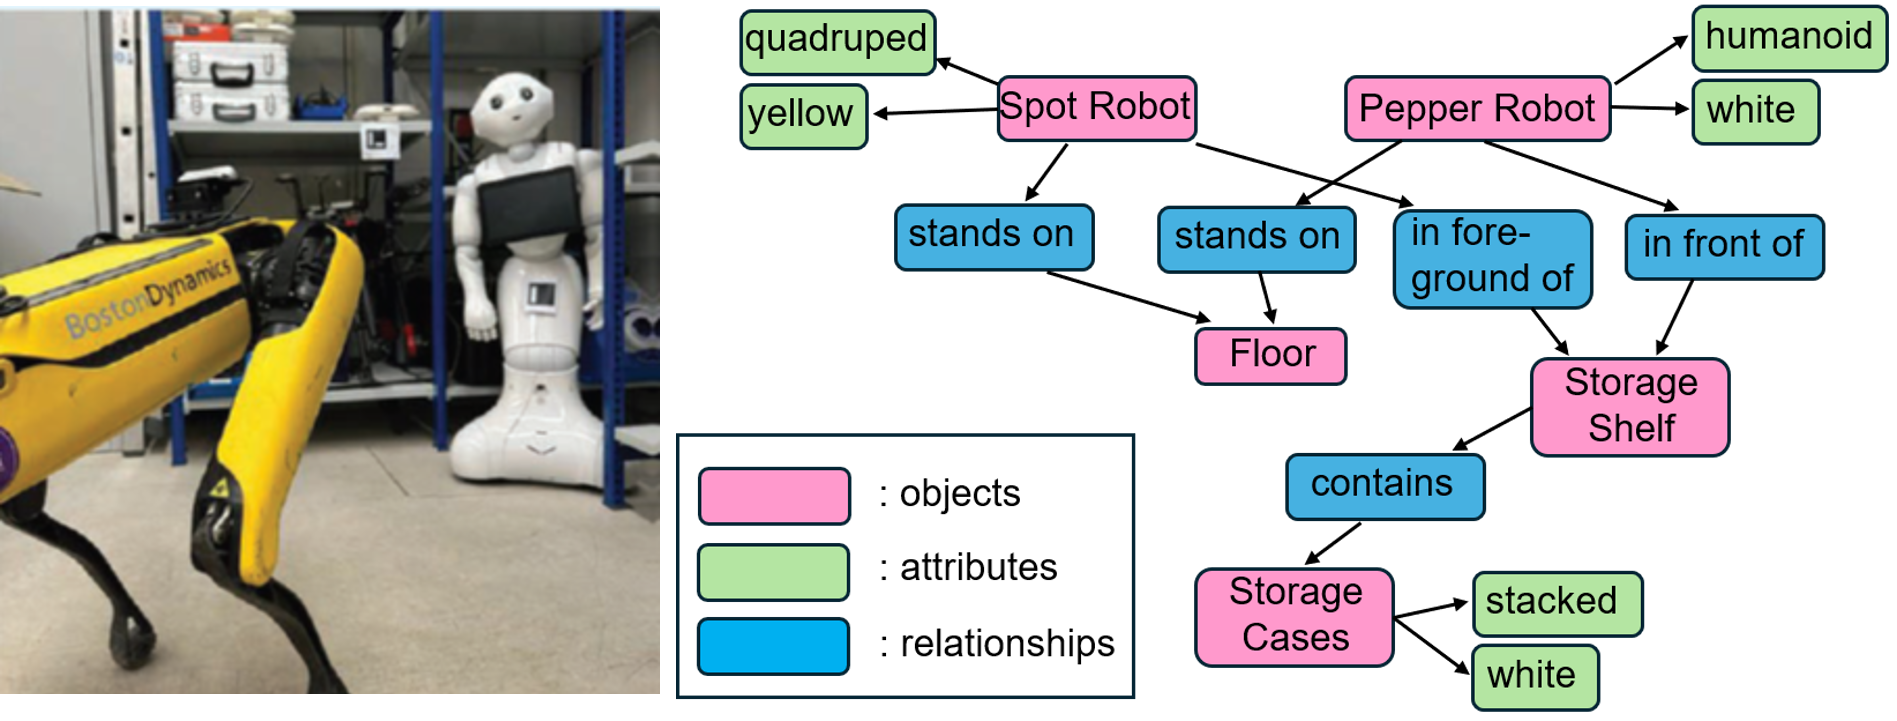
\includegraphics[width=\columnwidth]{Figures/SG_example_small.png}
    \caption{Example image of a scene (left) and related scene graph (right).}
    \label{fig:SG_example}
\end{figure}

The generation of scene graphs is mainly based on machine learning approaches and can be 
roughly divided into three parts: feature extraction, contextualization, and graph construction and reasoning \cite{li2024scene}. Herein, the process of feature extraction is mainly responsible for encoding objects or object pairs in the image. Contextualization plays the role of associating different
entities and is mainly used to enhance the contextual information between entities. Finally, 
this contextual information is used to predict the predicate and complete the construction and inference of the graph. There are currently two main types of scene graph generation \cite{li2024scene}, \cite{chang_comprehensive_2023}. The top-down methods comprise two sequential stages, namely object detection and pairwise relationship recognition, while the bottom-up method involves jointly detecting and recognizing the objects and their relationships \cite{adaimi2023composite}. 

As scene graphs can abstract objects and the relationships between them in a more explicit and easier-to-understand way, they became quite popular for visual scene understanding in general computer vision, but also in robotics. The conceptual shift from dense, low-level metric maps towards scene graphs represents a significant advancement in robotic world modeling. In robotics, scene graphs offer an abstract, layered representation that bridges the gap between the raw geometric perception and high-level symbolic reasoning \cite{bavle_slam_2023}. By decomposing an environment into a scene graph structure robots can move beyond flat representations, such as occupancy grids or point clouds, to models that capture the semantic and relational architecture of the world.  

As scene graphs might rapidly grow in real-world complex environments, the literature distinguishes between two primary structural paradigms: 
\begin{itemize}
    \item Flat Scene Graphs: these models treat all entities equally at a single level of representation, focusing on object-level nodes and their direct relationships \cite{catalano_3d_2025}. Approaches such as ConceptGraphs\cite{gu_conceptgraphs_2023} and SceneGraphFusion\cite{wu_scenegraphfusion_2021} utilize this approach to manage open-vocabulary object recognition and incremental updates in cluttered scenes where clear structural hierarchies may be emergent rather than predefined. 
    \item Hierarchical Scene Graphs: these represent the environment across multiple levels of abstraction, grouping lower level elements into semantically richer containers, e.g. objects within rooms, rooms within buildings\cite{rosinol_3d_2020} \cite{bavle_s-graphs_2025}. This multi-resolution approach is crucial for scalability in large-scale environments, as it allows robots to perform long-term planning and inference over compact abstractions rather than dense data \cite{catalano_3d_2025}.  
\end{itemize}
Hierarchical frameworks like Hydra \cite{hughes_hydra_2022} or S-Graphs\cite{bavle_s-graphs_2025} adopt a bottom-up stack comprising distinct layers specifically for indoor environments: (1) Metric-Semantic Mesh, Pointcloud, (2) Objects and Agents, (3) Places and Structures, (4) Rooms and Floors, and (5) Building. An example that extends these works to outdoor scenes is  \cite{greve_collaborative_2024} that proposes a hierarchical scene graph of a traffic scenario comprising 6 layers: (1) Keyframes \& Point clouds, (2) Lane Graph, (3) Vehicles, (4) Landmarks, (5) Roads \& Intersections, and (6) Environment.

As real-world scenes are three-dimensional, the idea of scene graphs has been extended to 3D space, leading to 3D scene graphs (3DSG) \cite{armeni_3d_2016} \cite{kim_3-d_2020}. 
Edges in a 3DSG encode the connections within the world model through several relationship types, such as: 
\begin{itemize}
    \item Spatial Relations: These include geometric constraints such as \textit{on}, \textit{in}, \textit{adjacent to} and \textit{support} \cite{catalano_3d_2025} \cite{yan_dynamic_2025}.
    \item Visibility and Proximity: \textit{Co-visibility} edges link objects seen simultaneously, while \textit{close-to} edges often use nearest-neighbor  k-d tree to define spatial proximity \cite{behrens_lost_2025}.
    \item Functional Relations: a newer class of edges representing operational dependencies. OpenFunGraph models these as directed edges between ``interactive elements'', such as switches and handles, and objects that they influence, e.g. \textit{controls} a light, \textit{opens} a cabinet \cite{zhang_open-vocabulary_2025}.
    \item Affordances: attributes or edges that define possible interactions which can change the entities' states, such as \textit{sit on}, \textit{opening}, \textit{pulling}, providing the robot with actionable knowledge \cite{catalano_3d_2025}.
    \item Containment and Affiliation: Inter-layer edges such as \textit{part of}, \textit{located in} or \textit{contains} facilitate hierarchical queries \cite{catalano_3d_2025} \cite{behrens_lost_2025}.
\end{itemize}
This structured abstraction allows robots to move beyond simple obstacle avoidance, static mapping and localization, towards actionable spatial perception, where the world model serves as a persistent, queryable memory for complex multi-step tasks in evolving robot-human shared spaces. Two examples of a 3DSG are shown in Figure \ref{fig:Examples_3DSG}.
\begin{figure}[ht]
    \centering
    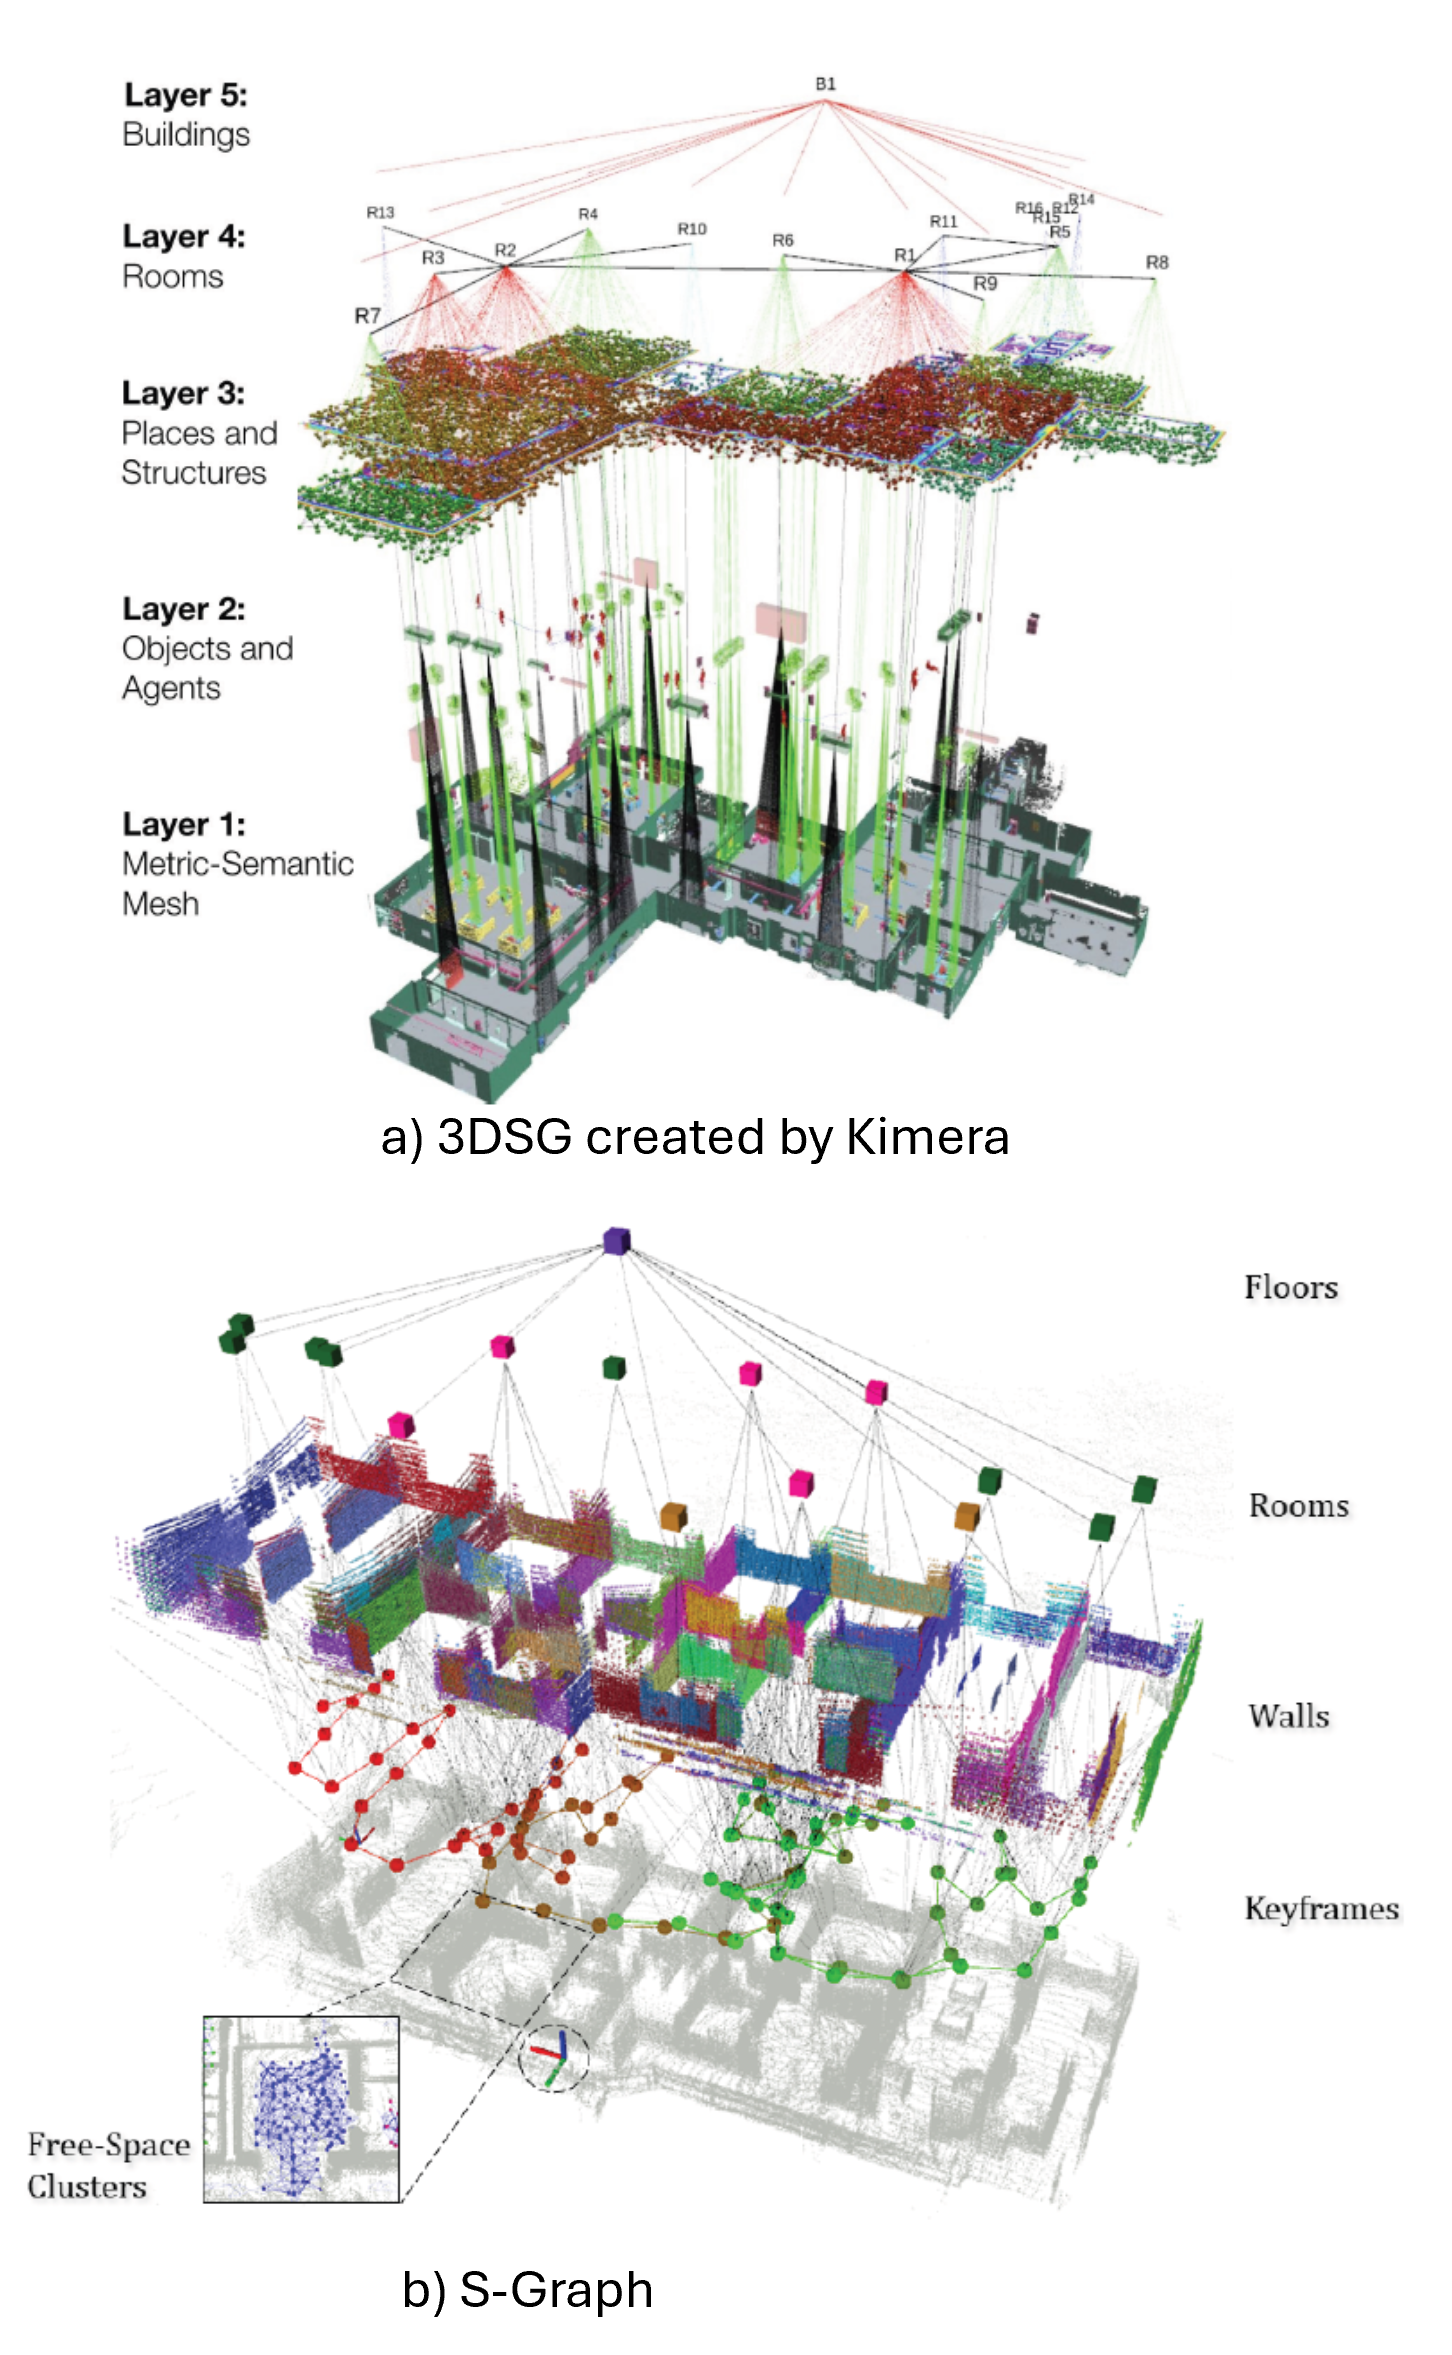
\includegraphics[width=\columnwidth]{Figures/Examples_3DSG.png}
    \caption{Example of 3DSGs created by (a) Kimera \cite{rosinol_kimera_2021} and (b) S-Graphs \cite{bavle_situational_2022}.}
    \label{fig:Examples_3DSG}
\end{figure}

\subsubsection{Hybrid Models using Factor and Scene Graphs}\label{sec:background_hybrid}
A scene graph answers \textit{``what exists and how it relates''}, while a factor graph answers \textit{``where it is, and how certain, consistent it is with sensor measurements''}.
This complementarity motivates hybrid architectures that combine the two paradigms within a common world representation, without implying that such architectures are generally superior to either paradigm in isolation.
Recent robotics 3DSG solutions explicitly include a pose-graph layer as the uncertainty-bearing backbone, and the integration of the two paradigms creates a multi-resolution framework which bridges metric-semantic perception with high-level symbolic reasoning \cite{rosinol_kimera_2021} \cite{bavle_situational_2022}.
In this hybrid paradigm, factor graphs serve as the probabilistic geometric backbone, while scene graphs provide the relational architecture necessary for task-level autonomy in dynamic environments \cite{catalano_3d_2025} \cite{rosinol_3d_2020}.

In this review, we use the term hybrid factor graph-scene graph (FG-SG) architecture in an operational sense. 
A system is considered hybrid when it explicitly maintains both a factor-graph-based estimation structure and a scene-graph representation of semantic entities and their relations, with explicit cross-representation correspondences between states or entities represented in the two structures.
This distinguishes hybrid FG-SG architectures from conventional semantic SLAM systems, in which semantic labels, object landmarks, or semantic priors may be incorporated into the SLAM graph without constructing a separate relational scene-graph representation.
Bidirectional information flow is not required for a system to be considered hybrid. Instead, the direction of information flow and, crucially, whether the two representations participate in a common optimization objective determine the form and degree of coupling.

% \hl{In this review, we use the term factor graph-scene graph (FG-SG) hybrid in an operational sense. 
% A system is considered hybrid when it explicitly maintains both a factor-graph-based estimation structure and a scene-graph representation of semantic entities and their relations, with an explicit correspondence or information exchange between the two.
% This distinguishes FG-SG hybrids from conventional semantic SLAM systems, in which semantic labels, object landmarks, or semantic priors may be incorporated into the SLAM graph without constructing a separate relational scene-graph representation.
% The existence of bidirectional feedback is therefore not required for a system to be considered hybrid, rather, the direction and magnitude of this information exchange determine its degree of coupling.} 

The literature converges to a small set of recurring architectural patterns for coupling the two paradigms, distinguished primarily by information-flow direction and optimization ownership. 
We first distinguish loosely coupled architectures, in which the factor graph and scene graph remain outside a common optimization objective, from tightly coupled architectures, in which scene-graph-level entities or constraints participate directly in the estimation graph. 
Within the loosely coupled class, we further distinguish layered/feed-forward and parallel architectures according to whether the scene graph is constructed downstream from the factor-graph output or maintained as a separate representation.

The first loosely coupled pattern is the \textbf{layered, feed-forward} \textbf{stack with factor graph backbone}: the factor graph simultaneously optimizes the robot's trajectory and the metric-semantic mesh, whose globally and temporally consistent output is then fed to a separate scene graph parser that builds the relational structure on top. 
Hydra \cite{hughes_hydra_2022} and Kimera \cite{rosinol_kimera_2021} support this approach, where a dedicated parsing thread incrementally constructs the scene graph from the optimized metric layer. 
The advantage is modularity, where the scene graph logic can be developed independently of the SLAM back-end, but the disadvantage is a one-directional information flow: the scene graph is informed by the factor graph, but semantic information rarely propagates back to improve localization.

The second loosely coupled pattern is the  \textbf{parallel architecture}, in which  the factor graph and scene graph are maintained as separate representations   and synchronize corresponding entity states or node positions through explicit cross-representation correspondences. Unlike the layered feed-forward case, the scene graph is maintained as a persistent representation rather than being constructed solely as a downstream product of the factor-graph output. Unlike the unified case, however, scene-graph-level states and constraints do not participate in the factor graph's optimization objective. This preserves modularity and reduces optimization complexity at the expense of weaker consistency guarantees \cite{rosinol_3d_2020}.

The tightly coupled pattern is the \textbf{unified optimizable graph}, in which scene graph entities are incorporated directly as variables and factors within the same factor graph that optimizes robot poses. 
S-Graphs \cite{bavle_s-graphs_2025} and its visual counterpart vS-Graphs \cite{tourani2026vs} introduced this pattern, merging SLAM and scene graph into a single multi-layered jointly optimizable factor graph where walls, rooms, and floors appear as semantic variables constrained by geometric factors.
This enables bidirectional information flow: geometric observations constrain semantic entity positions, but semantic structural priors in turn constrain and regularize ego-trajectory estimation, demonstrably reducing drift compared to purely geometric approaches.
The defining distinction from loosely coupled architectures is therefore participation of scene-graph-level states or constraints in the common estimation objective, rather than bidirectional information exchange alone.
\hl{The degree of architectural coupling should also be distinguished from the extent of uncertainty propagation.
A loosely coupled architecture can explicitly transfer uncertainty estimates between its constituent representations without performing joint optimization. Conversely, joint optimization does not necessarily imply that all uncertainty classes are explicitly modeled or that their posterior uncertainties are computed and made available to other representation layers.}

\subsection{Dynamics in the Context of Robotics}\label{sec:background_dynamics_definition}
It is necessary to fix what we mean by \textit{dynamics}, since the term is used inconsistently across robotics and adjacent fields. 
In classical mechanics, dynamics concerns forces and torques and their effect on motion; in dynamical system theory, it describes the time-evolution of a point in a geometric state space; in computer science, a ``dynamic'' data structure refers to memory organization rather than physical change. 
Within mobile robotics, the term is used more narrowly and typically refers to external, uncontrolled moving entities, such as pedestrians and vehicles, that a robot must perceive and account for during localization and mapping\cite{kucner_survey_2023}. 

This robotics-specific usage, however, is itself too narrow for our purpose.
Hahnel et al. \cite{hahnel2003map} offered one of the first attempts to define dynamics as an environmental property, stating that an environment is dynamic if it changes over time or if moving objects are present within it. 
This definition is useful but indirect, and, being framed around discrete macroscopic objects, does not make explicit how motion that is never directly observed, e.g. a chair found in a new location, should be treated. Therefore, we adopt the definition of dynamics given in \cite{kucner_survey_2023}:
\vspace{6pt}
\begin{definition}[Dynamics]
\label{def:dynamics}
    Dynamics are any directly or indirectly perceivable motions.
\end{definition}
\vspace{6pt}
This formulation is deliberately broad. \textit{Direct} perceivability covers motion observed as it occurs given an appropriate sensor.
\textit{Indirect} perceivability covers semi-static entities, such as relocated furniture, whose motion is never itself observed but whose resulting change of state is.
This distinction between direct and indirect perceivability, rather than any specific list of entity types or timescales, is what we take to be the essential content of Definition \ref{def:dynamics}, and it is this distinction, not a fixed taxonomy, that Kucner et al. \cite{kucner_survey_2023} leave open for further specialization within a given application domain.

Definition \ref{def:dynamics} tells us \textit{what} qualifies as dynamics. It does not by itself prescribe how a world model should organize or respond to different instances of it.
In Section \ref{sec:taxonomy_dynamics}, we build on this definition to introduce a taxonomy of dynamics tailored to graph-based robotic world models, organized primarily around the temporal horizon at which a perceivable motion or change occurs.

\begin{comment}
 
In the previous sections, we relied on an intuitive under-
standing of such fundamental terms as dynamics or maps.
However, both terms are widely used across different fields,
and their definitions vary from field to field. For instance, in
the field of classical mechanics, dynamics concern the study
of forces and torques and their effect on motion. A dy-
namical system in mathematics refers to a system in which a
function describes the time dependence of a point in a
geometrical space. In computer science, a dynamic data
structure refers to an organization or collection of data in
memory that has the flexibility to grow or shrink in size.
In the context of mobile robotics the term dynamics is
much less ambiguous and is usually used to describe ex-
ternal, uncontrolled moving entities. That said, this term is
not often used in relation to environmental features. Thus, to
apply this term in the context of MoDs, there is a need to
redefine it. The first attempt to define dynamics as an en-
vironmental feature was proposed by H¨ahnel et al. (2003).
In their work, the authors state that an environment is
dynamic if it changes or if moving objects are present
therein. This indirect definition of dynamics is formulated
such that it primarily focuses on macroscopic objects.
Meanwhile, contemporary robotics finds its application in a
multitude of environments where not only macroscopicdiscrete objects are dynamic. In fields like aerial and marine
robotics, the dynamics also include the flow of water and air,
respectively. Thus, the definition by H¨ahnel et al. (2003)
does not cover such types. To mitigate this limitation, we
propose the following definition of dynamics in the context
of robotics:
\begin{definition}[Dynamics]
\label{def:dynamics}
Dynamics are any directly or indirectly perceivable motions.
\end{definition}
Such a formulation of dynamics captures both motion of
discrete objects and continuous media (they are both per-
ceivable with adequate sensors, that is, anemometers,
speedometers, radars)
This definition further includes semi-static objects. For
such objects (i.e. chairs, cars), the motion is not per-
ceivable directly (the motion of an actual object has not
been perceived), but the result (indirect observation) can
be.
\end{comment}

\subsection{Assessment of Previous Surveys and Reviews}
% FG
Probabilistic Graphical Models provide the foundational framework for modeling large-scale inference problems in robotics, with factor graphs serving as a bipartite representation where variables denote unknown states and factors represent local constraints derived from sensor data \cite{dellaert_factor_2021} \cite{dellaert_factor_2017}.
Traditional reviews trace the maturity of SLAM from early formulations based on Kalman filters and Bayesian estimation toward modern graph-based optimization paradigms \cite{mascaro_scene_2025} \cite{luca_carlone_slam_2025}.
Systematic surveys of spatial perception frameworks have categorized scene modeling techniques into three primary layers: metric, metric-semantic, and metric-semantic-topological \cite{mascaro_scene_2025}. 
This highlights a trend shifting away from purely geometric representations like point clouds or meshes, toward advanced data structures that incorporate high-level concepts such as instances and places \cite{bavle_slam_2023}.

% SG
Complementary to reviews of metric frameworks, existing reviews of scene graphs define them as structured representations that encode semantic entities and their interrelationships to facilitate human-like reasoning \cite{chang_comprehensive_2023} \cite{amuche_advancements_2025} \cite{lai_review_2022}. 
Early literature in this domain primarily focused on offline image retrieval and 2D scene graph generation, though more recent reviews highlight advancements in 3D scene graphs capable of capturing metrics, semantics and objects (also including dynamic agents) within a unified actionable model \cite{chang_comprehensive_2023} \cite{lai_review_2022}.

Notably, these two types of reviews have developed largely independently: reviews of factor graphs assess uncertainty-aware geometric estimation, while reviews of scene graphs assess semantic and relational abstraction, but very few works survey both representations \emph{jointly} as complementary layers of a single world model. A first recent attempt in this direction is the review of Catalano et al. \cite{catalano_3d_2025}, which focuses on works that combine geometry, semantics, and action within unified representations; however, this overview  does not center on dynamics, nor does it systematically analyze the coupling patterns, uncertainty propagation, or construction pipelines that arise when factor and scene graphs are combined specifically to handle non-stationary environments.

% Dynamic SLAM
The landscape of SLAM in dynamic environments has been analyzed as a progressive evolution from purely geometric methods to advanced semantic-based paradigms \cite{wang_survey_2024} \cite{chen_semantic_2025} \cite{wen_semantic_2021}.
Existing surveys categorize solution approaches into those that maintain localization stability by excluding dynamic elements as outliers and those that perform active Simultaneous Localization, Mapping and Moving Object Tracking (SLAMMOT) \cite{wang_-depth_2025} \cite{xu_survey_2021}. 
Furthermore, dedicated reviews on feature requirements in dynamic SLAM weight the trade-offs between low-level primitives, such as points or lines, and high-level semantic labels, suggesting that robust robotic autonomy may require the integrated usage of both feature levels \cite{xu_survey_2021}.
These dynamic-SLAM surveys, however, largely set aside the scene-graph literature, and consequently do not address how semantic-relational structure should be maintained under dynamics, nor how it interacts with the probabilistic backbone of the factor graph.

A separate line of work addresses dynamics as a phenomenon in its own right, independent of any specific representation. Kucner et al.\cite{kucner_survey_2023} survey Maps of Dynamics (MoDs) and propose a general definition and characterization of dynamics for mobile robotics, which we adopt and extend in Section \ref{sec:background_dynamics_definition} and organize into a temporal-horizon taxonomy in Section~\ref{sec:taxonomy_dynamics}. 
While their survey provides a rigorous treatment of \textit{what} dynamic phenomena are and how they can be statistically modeled over space and time, it is agnostic to the underlying world-model representation, and does not address factor graphs, scene graphs, or their hybrid forms.

% Identified gaps
Despite the depth of reviews in individual subfields, critical gaps in the existing review or survey literature can be identified.  
Key surveys often focus on isolated areas like perception or planning while overlooking the practical integration of these components \cite{khan_foundation_2025} \cite{bavle_slam_2023}.
Gaps also remain in analyzing the long-term usability of maps in complex dynamic scenes and handling the non-rigid deformations inherent in highly dynamic environments \cite{chen_semantic_2025} \cite{luca_carlone_slam_2025}.
Taken together, these limitations reveal a fragmented landscape in which probabilistic estimation (factor graphs), semantic scene understanding (scene graphs), and the characterization of dynamics have each matured in relative isolation, with limited cross-pollination between the three. 
To the best of our knowledge, no existing survey or review jointly addresses the full pipeline from probabilistic spatio-temporal estimation to structured semantic reasoning especially in \textit{dynamic} environments, nor does any work systematically analyze how these two paradigms can be combined to achieve robust, long-term or even lifelong situational awareness.

This review addresses these gaps directly.
We first establish a shared characterization of dynamics (Section~\ref{sec:taxonomy_dynamics}), building on and extending the definition of Kucner et al. \cite{kucner_survey_2023} and based on the surveyed literature, and then assess existing works with respect to three questions: which graph-based representations are suited to dynamic environments (Section ~\ref{sec:dyn_world_model_representations}), how they are constructed and maintained (Section ~\ref{sec:construction_pipeline}), and how they are exploited for downstream tasks (Sections~\ref{sec:querying_reasoning_action}--\ref{sec:applications}). 
Additionally, we present the commonly used evaluation protocols, datasets, and metrics for testing in ~\ref{sec:evaluation_metrics}, and a  structured comparison of  representative related works in ~\ref{sec:taxonomy}. Finally, we conclude this review by highlighting the open challenges identified and outlining future research directions in ~\ref{sec:challenges_future_works}. 
In doing so, this review provides a unified perspective on the synergy between factor graphs and scene graphs as complementary and mutually reinforcing tools for long-term robotic autonomy under dynamics.


\subsection{Review Scope and Literature Selection}
The literature corpus was assembled through targeted searches of IEEE Xplore, Google Scholar, and arXiv, complemented by backward and forward citation tracing from key surveys and representative works.
The primary search covered publications from 2012 to July 2026, while earlier works were retained where needed to establish methodological foundations.
Search concepts combined terms related to \textit{factor graphs}, \textit{scene graphs}, \textit{dynamic SLAM}, \textit{dynamic world models}, \textit{spatio-temporal mapping}, \textit{lifelong mapping}, \textit{multi-object tracking}, and \textit{semantic/relational mapping}.
% We included robotic systems that employ factor graphs, scene graphs, or their combination to represent, construct, maintain or exploit world models under environmental dynamics.
% Static-only mapping, perception-only methods without a persistent world representation, and works outside robotics were excluded unless directly relevant to the emerging trends discussed in this review. 
% The systems in Table} \ref{tab:taxonomy_overview} \hl{were selected as representative examples spanning the main graph-stack architectures, dynamic regimes, inference strategies, uncertainty treatments, and downstream uses identified in the survey.
% As a topical rather than systematic review, the resulting corpus is intended to be broad and representative rather than exhaustive, particularly for the rapidly evolving preprints and adjacent emerging representations.
Candidate works were included when they: (i) addressed a robotic mapping, world-modeling, tracking or scene-understanding problem; (ii) employed factor graphs, scene graphs, or their combination as a substantive component of the maintained representation or inference architecture; and (iii) addressed environmental dynamics or contributed directly to one of the representation, construction/maintenance, or exploitation questions considered in this review.
Earlier static or methodological works were retained when required to establish the foundations of techniques subsequently used for dynamic world modeling.
Static-only mapping systems, perception-only methods without a persistent world representation, and works outside robotics were excluded unless directly required for methodological context.
The comparative systems in Table \ref{tab:taxonomy_overview} constitute a representative rather than exhaustive subset of this corpus. 
Systems were selected when they instantiated one of the main FG, SG, or hybrid architectural patterns identified in the review, treated environmental dynamics as a substantive part of the method, and provided sufficient information to characterize the comparison axes introduced in Section \ref{sec:taxonomy}. Where several closely related works instantiated the same architecture, preference was given to the most complete or representative system description, while other works were retained when they introduced a distinct formulation or capability.

The review adopts a structured topical-review methodology designed to provide broad coverage of the principal graph-based approaches to dynamic robotic world modeling.
The combination of database searches, citation tracing and explicit selection criteria was used to capture the main methodological developments, architectural patterns, and representative systems relevant to the scope of the review.
Given the breadth and rapid evolution of the field, the identified trends and research gaps should be interpreted within the scope and selection criteria defined above.

\section{Taxonomy of Dynamic Aspects in Robotic World Models}\label{sec:taxonomy_dynamics}
Before analyzing how factor graphs and scene graphs represent, construct and exploit non-stationary environments, we first set the vocabulary this review adopts to describe \textit{dynamics themselves}. 
The literature is not consistent here: the same underlying phenomenon, e.g., a chair being moved between visits, is variously described as a \textit{semi-static change} \cite{gomez_object-based_2020}, a \textit{movable} object \cite{brink_using_2016} or a node with a \textit{persistence} attribute\cite{behrens_lost_2025}.
Establishing a shared characterization upfront allows us to classify representations, pipelines, and applications along consistent axes for the remainder of the review.

We organize dynamics along three axes: 
\emph{when} a change occurs relative to observation (Temporal Horizon),
\emph{what} kind of entity undergoes it (Entity Typology),
and \emph{how} the change manifests in the representation (State Expression).
A fourth property, the \emph{predictability} of a dynamic entity's behavior, is briefly noted at the end of this section since it is only sparsely addressed by the surveyed literature.

\subsection{Primary Axis: Temporal Horizon}\label{sec:taxonomy_temporal_horizon}

\begin{table}[t]
\centering
\scriptsize
\setlength{\tabcolsep}{3pt}
\renewcommand{\arraystretch}{1.15}
\caption{Primary temporal-horizon axis used to organize dynamics in graph-based robot world models.}\label{tab:temporal_horizon_taxonomy}
    \begin{tabularx}{\columnwidth}{@{}p{0.15\columnwidth} p{0.12\columnwidth} X@{}}
    \toprule
    \textbf{Tier} & \textbf{Observation-relative criterion } & \textbf{Description} \\
    \midrule
    Short-Term Dynamics 
    &  Evolves during continuous observation 
    &  Motion must be estimated during observation, such as humans, vehicles, or robots \\ 
    \midrule
    Semi-Static Changes 
    &  Stable within observation, changes between observations/revisits 
    &  Relocation, appearance/disappearance, or persistent state transitions such as open/closed door \\ 
    \midrule
    Long-Term Structural Changes 
    &  Persistent structural modification across sessions 
    &  Changes to the built environment itself, such as layout changes, renovations, or seasonal structural variations  \\
    \bottomrule
    \end{tabularx}
\end{table}
% \begin{table}[t]
% \centering
% \caption{Primary temporal-horizon axis used to organize dynamics in graph-based robot world models.}\label{tab:temporal_horizon_taxonomy}
%     \begin{tabularx}{\columnwidth}{@{}p{0.12\columnwidth} p{0.12\columnwidth} X X@{}}
%     \toprule
%     \textbf{Tier} & \textbf{Timescale} & \textbf{Description} & \textbf{Required model mechanism} \\
%     \midrule
%     Dynamic Agents 
%     & Continuous / Now 
%     & Independently moving entities whose pose changes during observation, such as humans, vehicles, or robots 
%     & Real-time tracking, motion-aware data association, and often joint SLAMMOT-style estimation \\
%     \midrule
%     Semi-Static Changes 
%     & Minutes--Days 
%     & Entities that are static during a single observation but may be relocated, added, removed, or change state between observations 
%     & Persistence reasoning, object permanence, containment relations, and state-update policies \\
%     \midrule
%     Long-Term Structural Changes 
%     & Days--Years 
%     & Persistent modifications to the built environment itself, such as layout changes, renovations, or seasonal structural variations 
%     & Multi-session alignment, change detection, map repair, and lifelong graph maintenance \\
%     \bottomrule
%     \end{tabularx}
% \end{table}

The dimension that structures most consistently both individual models and this review is \textit{when} a change occurs relative to the robot's observation stream, since it directly governs the memory allocation, data association strategy, and update frequency a world model must support. 
We distinguish three tiers:

\begin{itemize}
    \item \textbf{Short-Term Dynamics} ( within-observation evolution): humans, moving vehicles, and other independently moving entities whose pose changes within the timescale of a single operating session, requiring real-time tracking and motion-aware data association \cite{bescos_dynaslam_2021} \cite{morris_dynosam_2025} \cite{schmid_khronos_2024}.
    \item \textbf{Semi-Static Changes} ( between-observation state changes): objects that are stationary during any single observation but relocated, added, removed, or state-transitioned between observations, e.g., furniture rearrangement or a door's open/closed state \cite{gomez_object-based_2020} \cite{giberna_dynemo-slam_2025} \cite{schmid_khronos_2024}.
    \item \textbf{Long-Term Structural Changes} ( persistent cross-session evolution): modifications to the built environment itself, e.g., renovations or seasonal layout shifts, requiring inter-session alignment and lifelong map maintenance \cite{walcott-bryant_dynamic_2012} \cite{kim2022lt}.
\end{itemize}
These tiers classify motion and state-change processes, rather than physical entities themselves.
Temporal Horizon is defined relative to the robot's observation process and world-model update cycle, rather than by a universal elapsed-time threshold.
\hl{Although these regimes are typically associated with different orders of magnitude in elapsed time, such temporal ranges are only indicative and do not define classification boundaries.
The classification depends on the frequency and continuity of observations, the operational context of the robot, and the persistence and structural nature of the environment change. 
For instance, the same object displacement may be perceived as continuous motion by a robot directly observing it, or a semi-static change by a robot revisiting the scene after the displacement occurred. }
A change process is classified as \textbf{short-term} when its state evolves during continuous observation and must therefore be estimated or tracked online; as \textbf{semi-static} when the entity is approximately stationary within an observation but its state differs between observations or revisits; and as \textbf{long-term structural} when the change constitutes a persistent modification of the environment's structural configuration across sessions or deployments. 
Consequently, different dynamic processes associated with the same physical entity may belong to different tiers, and may coexist within the same world model. 
For example, the articulated trajectory of a door while it is opening is a short-term dynamic process, the resulting open/closed state retained between observations is a semi-static state change, and installation, removal, or persistent reconfiguration of the door or doorway constitutes long-term structural evolution.
The taxonomy is therefore operational rather than object-specific. The three regimes imply different representation and maintenance requirements, ranging from continuous motion estimation and tracking, through state persistence and transition reasoning, to multi-session structural change detection and map restructuring.

% \hl{These tiers should be interpreted as operational temporal regimes rather than mutually exclusive classes of physical entities.
% The classification applies to a particular motion or state-change process relative to the robot's observation horizon and task requirements. Consequently, the boundaries between tiers are intentionally approximate and application-dependent.
% The same physical entity may therefore participate in multiple temporal regimes. 
% A door, for instance, can exhibit short-term articulated motion while being opened or closed, retain semi-static open/closed state across observations, and undergo a long-term structural change if the door or doorway is permanently installed, removed, or reconfigured. 
% Accordingly, a world model may represent different state variables or change process associated with the same entity at different temporal horizons. 
% }

This tiering is not merely descriptive: it maps directly onto the mechanism a world model must implement, from the tightly-coupled SLAMMOT formulations used for Short-Term Dynamics, through the persistence and containment reasoning used for Semi-Static Changes, to multi-session change detection used for Long-Term Structural Changes. 
We adopt this three-tier distinction as the primary organizing axis for the remainder of the paper.
A summary is depicted in Table \ref{tab:temporal_horizon_taxonomy}.

\subsection{Secondary Axes: Entity Typology and State Expression}\label{sec:taxonomy_secondary_axes}
Within each temporal tier, two further properties are useful for characterizing \textit{what} is changing and \textit{how} that change is expressed in the graph. 
Table \ref{tab:dynamics_taxonomy} summarizes both.

\textbf{Entity Typology} distinguishes dynamic elements by the structural assumption their motion model requires. 
\textit{Rigid} entities undergo $SE(3)$ pose change with constant geometry and dominate the surveyed factor-graph formulation \cite{bescos_dynaslam_2021} \cite{qiu2022airdos}.
\textit{Articulated} entities are constrained by internal kinematic chains, relevant both to manipulable objects such as doors and drawers \cite{zhang_open-vocabulary_2025} and to parametric human body models \cite{henning_bodyslam_2022} \cite{henning_bodyslam_2023}.
\textit{Deformable} entities, whose shape or topology changes non-rigidly, remain largely outside the scope of the probabilistic graph-based systems surveyed here.

\textbf{State Expression} distinguishes \textit{how} a change manifests once represented. 
\textit{Geometric-kinematic} changes are variations in position, velocity, or boundary and are the traditional target of factor graph estimation.
\textit{Semantic-affordance} changes affect an entity's functional or operational state, e.g., a light turning on or off, and are typically encoded as node attributes in 3D scene graphs \cite{catalano_3d_2025} \cite{olivastri_multi-modal_2024}.
\textit{Topological} changes modify the connectivity of the environment itself, e.g., a closed door removing the traversable edge between two rooms, and are of particular relevance to hierarchical scene graph maintenance \cite{catalano_3d_2025}.

\begin{table}[t]
\centering
\scriptsize
\setlength{\tabcolsep}{3pt}
\renewcommand{\arraystretch}{1.15}
\caption{Secondary axes used to characterize dynamic entities within each
temporal tier.}\label{tab:dynamics_taxonomy}
    \begin{tabularx}{\columnwidth}{@{}l l X@{}}
    \toprule
    \textbf{Axis} & \textbf{Category} & \textbf{Description} \\
    \midrule
    \multirow{3}{*}{\shortstack[l]{Entity\\Typology}}
     & Rigid       & $SE(3)$ pose change, constant geometry \\
     & Articulated & Kinematic chain, constrained internal DoF \\
     & Deformable  & Non-rigid shape/topology change \\
    \midrule
    \multirow{3}{*}{\shortstack[l]{State\\Expression}}
     & Geometric-Kinematic  & Position, velocity, boundary change \\
     & Semantic-Affordance  & Functional/operational state change \\
     & Topological          & Connectivity change in the scene graph \\
    \midrule
    \midrule
    \multirow{3}{*}{\shortstack[l]{Behavioral\\Intent}}
     & Deterministic  & Motion strictly governed by fixed laws \\
     & Physics-Based  & Motion governed by physics-based probabilities \\
     & Goal-Driven    & Motion governed by internal decisions or social compliance \\
    \bottomrule
    \end{tabularx}
\end{table}

\subsection{Adopted Characterization}\label{sec:taxonomy_adopted_characterization}
We adopt \textbf{Temporal Horizon} as the primary organizing dimension of this review, using the three-tier distinction to structure this paper's analysis.
The tiers are not mutually exclusive labels for entities or systems. They characterize change processes at different observation horizons, and a single entity or world model may simultaneously instantiate more than one tier.
Entity Typology and State Expression are used as secondary, descriptive dimensions throughout, applied where relevant to characterize individual systems without constituting an independent organizational axis.
A fourth property, \textit{Behavioral Intent}, that is the degree to which a dynamic entity's future motion is deterministic, physics-based or goal-driven, is addressed by only a small subset of the reviewed literature \cite{catalano_aion_2025} \cite{gorlo_long-term_2024} and remains largely decoupled from probabilistic world-model construction.
%We revisit it explicitly as an open direction in Section \ref{sec:open_challenges}

\begin{comment}

When building a general taxonomy for dynamic aspects in robotic world models, the goal is to categorize how a robot perceives, tracks, predicts, and reasons about a world that is not frozen in time. A general taxonomy of dynamic aspects in robotic world models can be structured around four interconnected pillars. This framework defines how a robot perceives, maintains, and projects environmental changes over time:
\begin{enumerate}
    \item \textbf{Entity Typology (The "What")} This dimension classifies the structural and material properties of the moving or changing elements, which dictates how they must be mathematically modeled:
    \begin{itemize}
        \item Rigid Dynamics: $SE(3)$ pose changes where geometry remains constant (e.g., vehicles, pedestrians).
        \item Kinematic Chains: Articulated objects with constrained internal degrees of freedom (e.g., opening doors, drawers).
        \item Deformable Elements: Non-rigid materials that change shape or topology (e.g., cables, cloth, liquids).
        \item Substance Fields: Continuous environmental phenomena lacking discrete boundaries (e.g., smoke, changing illumination).
    \end{itemize}
    \item \textbf{State Expression (The "How")} Dynamism manifests as changes in either the spatial layout or the internal characteristics of the world:
    \begin{itemize}
        \item Geometric-Kinematic Dynamics: Trackable variations in position, velocity, and physical boundaries.
        \item Semantic-Affordance Dynamics: Changes in the operational state or functional availability of an object (e.g., a stove turning "ON", a container becoming "Full").
        \item Topological Dynamics: Modifications to the connectivity of the environment (e.g., a closed door breaking the traversable edge between a hallway and a room). 
     \end{itemize}
    \item \textbf{Temporal Horizons (The "When")}
    This dimension governs the memory allocation, data association, and updating frequency required by the world model:
    \begin{itemize}
     \item Transient (Short-Term): High-frequency, immediate changes (seconds to minutes) requiring real-time tracking and collision avoidance.
     \item Episodic (Medium-Term/Semi-Static): Intermittent changes occurring between observations (hours to weeks), requiring change detection and graph-mutation (e.g., relocated furniture).
     \item Structural (Long-Term): Permanent or seasonal changes (months to years) requiring lifelong map maintenance and the discarding of stale environmental anchors.
    \end{itemize}
    \item \textbf{Behavioral Intent (The "Why")}
    This categorizes the predictability of the dynamic element, moving from reactive tracking to proactive anticipation:
    \begin{itemize}
    \item Deterministic: Motion strictly governed by fixed laws or periodic schedules (e.g., a conveyor belt).
    \item Stochastic-Kinematic: Motion governed by physics-based probabilities (e.g., a vehicle maintaining a constant velocity model with noise).
    \item Intentional/Social: Goal-driven motion governed by internal decisions or social compliance (e.g., a human walking toward a specific tool, obeying traffic rules).
    \end{itemize}
\end{enumerate}
\end{comment}

\section{Graph-Based Robotic World Models For Dynamic Environments}\label{sec:dyn_world_model_representations}
The evolution of world model representation in robotics has undergone a significant paradigm shift, transitioning from rigid, static geometric maps to adaptive, spatio-temporal structure capable of handling and reasoning about dynamic environments \cite{bavle_slam_2023} \cite{rosinol_kimera_2021}.
In this section, we first review factor graphs as geometric probabilistic backbones (Section \ref{sec:dyn_world_model_representations_factor_graphs}), scene graphs as semantic abstractions (Section \ref{sec:dyn_world_model_representations_scene_graphs}) in dynamic environments, and finally discuss how dynamics themselves are represented (Section \ref{sec:dynamics_representations}).

\subsection{Representational Foundations}
\subsubsection{Factor Graphs as Dynamic Geometric World Models}\label{sec:dyn_world_model_representations_factor_graphs}
To mitigate the impact of outliers and non-stationarity in dynamic environments, factor graph-based systems employ a range of probabilistic robustness mechanisms.
A common approach is the use of \textbf{robust cost functions}, such as the Huber loss, which reduce the influence of large residuals during nonlinear least-squares optimization while preserving sensitivity to small, consistent measurement errors\cite{song_rts-slam_2025}. 
This allows the optimizer to tolerate transient violations of the static-world assumption, caused for instance by moving objects or short-time occlusions, without destabilizing the global solution.
Complementary to robust kernels, \textbf{dynamic information reweighting strategies} explicitly modulate the contribution of individual factors based on their consistency with the current state estimate \cite{lingzhu_xiang_robust_2015}. 
Techniques such as Dynamic Covariance Scaling (DCS) or switchable constraints introduce latent scaling variables that adaptively downweight measurements whose residuals are incompatible with the inferred global structure, providing a principled outlier rejection.
Beyond measurement-level robustness, more expressive models introduce \textbf{latent mobility or existence variables} associated with landmarks or objects, which explicitly encode the likelihood that an entity linked to that variable is static, movable, or currently in motion \cite{lingzhu_xiang_robust_2015}.
By scaling the corresponding factor covariances or relaxing constraints when mobility is inferred, these approaches prevent dynamic or semi-static entities from corrupting the static map while still allowing them to be represented within the same probabilistic framework.
Together, these mechanisms transform factor graphs from purely static geometric estimators into uncertainty-aware models capable of reasoning under dynamic, partially observable conditions.
% To mitigate the impact of outliers in dynamic environments, such as moving objects or spurious loop closures, explicit probabilistic techniques are employed:
% \begin{itemize}
%     \item Robust Kernels: The Huber cost function is frequently applied to downweight large residual, providing a robust optimization back-end that prevents the solution from degrading due to extreme outliers while balancing sensitivity to small residuals\cite{song_rts-slam_2025}.
%     \item Dynamic Scaling: mechanisms like Dynamic Covariance Scaling (DCS) or switchable constraints regularize Mahalanobis errors by dynamically scaling the information matrices of individual edges based on their consistency with the global state \cite{lingzhu_xiang_robust_2015}.
%     \item Latent Mobility Variables: advanced models introduce scalar latent parameters ($\mathit{w}_j$) for each landmark, effectively scaling the covariance to loosen constraints for moving/movable entities, pushing their distribution toward uniformity and neutralizing their influence on the static map \cite{lingzhu_xiang_robust_2015}.
% \end{itemize}
Recently, many works \cite{bescos_dynaslam_2021} \cite{giberna_dynemo-slam_2025} \cite{brink_using_2016} \cite{deeb_model-based_2019} have integrated semantic priors transforming the factor graph from a purely geometric map into a context-aware reasoning engine, facilitating the coupling with other graphical models such as scene graphs.  

Traditional SLAM systems are optimized for a static world treating moving objects and agents as outliers to be rejected \cite{bescos_dynaslam_2018} \cite{bavle_s-graphs_2025}. 
Modern dynamic SLAM instead incorporates these dynamic entities into the graph, moving towards a coupled SLAMMOT approach that is examined in detail in Section \ref{sec:dynamics_representations_agents}.
%Modern dynamic SLAM instead incorporates these dynamic entities into the graph to simultaneously estimate camera trajectory and object motion, therefore enhancing the system robustness and the expressiveness of the resulting world model \cite{deeb_model-based_2019} \cite{gou_visual_2024} \cite{henein_dynamic_2020} \cite{morris_dynosam_2025}, moving towards a coupled SLAMMOT approach, combining SLAM and Multi-Object Tracking. 

\subsubsection{Scene Graphs as Structured Abstraction in Dynamic World Models}\label{sec:dyn_world_model_representations_scene_graphs}
\begin{comment}
The conceptual shift from dense, low-level metric maps towards 3D Scene Graphs represents a significant advancement in robotic world modeling. 
This offers an abstract, layered representation that bridges the gap between the raw geometric perception and high-level symbolic reasoning \cite{bavle_slam_2023}.
By decomposing an environment into a graph structure $G=(V,E)$ robots can move beyond flat representations, such as occupancy grids or point clouds, to models that capture the semantic and relational architecture of the world.  

The literature distinguishes between two primary structural paradigms for scene graphs: 
\begin{itemize}
    \item Flat Scene Graphs: these models treat all entities equally at a single level of representation, focusing on object-level nodes and their direct relationships \cite{catalano_3d_2025}. Systems such as ConceptGraphs\cite{gu_conceptgraphs_2023} and SceneGraphFusion\cite{wu_scenegraphfusion_2021} utilize this approach to manage open-vocabulary object recognition and incremental updates in cluttered scenes where clear structural hierarchies may be emergent rather than predefined. 
    \item Hierarchical Scene Graphs: these represent the environment across multiple levels of abstraction, grouping lower level elements into semantically richer containers, e.g. objects within rooms, rooms within buildings\cite{rosinol_3d_2020} \cite{bavle_s-graphs_2025}. This multi-resolution approach is crucial for scalability in large-scale environments, as it allows robots to perform long-term planning and inference over compact abstractions rather than dense data \cite{catalano_3d_2025}.  
\end{itemize}

Hiearchical frameworks like Hydra \cite{hughes_hydra_2022} and S-Graphs\cite{bavle_s-graphs_2025} adopt a bottom-up stack comprising distinct layers specifically for indoor environments:
\begin{enumerate}
    \item Metric-Semantic Mesh, Pointcloud.
    \item Objects and Agents.
    \item Places and Structures.
    \item Rooms and Floors
    \item Building.
\end{enumerate}
Extending these works to outdoor scenes, \cite{greve_collaborative_2024} proposed hierarchical 3D urban scene graph comprising 6 layers: 
\begin{enumerate}
    \item Keyframes \& Point clouds.
    \item Lane Graph.
    \item Vehicles.
    \item Landmarks.
    \item Roads \& Intersections.
    \item Environment.
\end{enumerate}
\end{comment}
Dynamics in scene graphs are typically handled through three complementary mechanisms operating at different temporal and semantic levels. 
\textbf{Spatio‑temporal consistency} is addressed by separating short‑term dynamics from long‑term structure: systems such as Khronos maintain a fast \textit{active window} to absorb immediate changes due to moving humans or objects, while a slower global process detects persistent changes and updates the long‑term scene graph accordingly \cite{schmid_khronos_2024}. 
Beyond short‑term consistency, some approaches explicitly model recurring temporal patterns. 
The Aion framework augments hierarchical scene graphs with \textit{Maps of Dynamics} (MoDs), attaching directional, time‑dependent \textbf{dynamic temporal flow} statistics to navigational nodes in order to capture typical or seasonal human motion patterns, while using \textit{Temporal Ownership Transfer} to preserve these dynamics under loop closures and graph reorganization \cite{catalano_aion_2025}. 
Finally, \textbf{belief and persistence reasoning} is used to cope with partial observability and object permanence. 
Belief Scene Graphs introduce probabilistic \textit{blind nodes} to represent entities expected to exist but not currently observed, inferred from learned commonsense co‑occurrence patterns \cite{saucedo_estimating_2025}, while interaction‑driven systems such as DovSG perform localized graph updates during human–object interactions, reflecting state changes without requiring a full scene rescan \cite{yan_dynamic_2025}.
Together, these approaches show an evolution of scene graphs from static semantic hierarchies toward persistent spatio-temporal memories that represent not only current scene state but also change, recurrence, and expected future activity.
% Dynamics in scene graphs are handled through various maintenance and prediction mechanisms: 
% \begin{itemize}
%     \item Spatio-Temporal Consistency: to manage changes like moving furniture and humans, systems like Khronos \cite{schmid_khronos_2024} factorize the problam into a fast \textit{active window} for short-term dynamics and a slower global process for long-term change detection.
%     \item Temporal Flow Dynamics: the Aion framework \cite{catalano_aion_2025} integrates Maps of Dynamics (MoDs) into hierarchical scene graphs, attaching directional flow statistics to navigational nodes to predict typical/seasonal human motion patterns over time. It uses Temporal Ownership Transfer to maintain consistency when nodes are repositioned during loop closures.  
%     \item Belief and Persistence: Belief Scene Graphs (BSG) employ probabilistic inference to estimate the existence of "blind nodes", i.e. unseen objects, based on commonsense co-occurance patterns \cite{saucedo_estimating_2025}. Other systems, such as DovSG \cite{yan_dynamic_2025}, perform local graph updates during interaction to reflect real-world state changes, e.g. an object being moved, without the need of a full scene rescan. 
% \end{itemize}

\begin{comment}
Edges in a 3DSG encode the connections within the world model through several relationship types: 
\begin{itemize}
    \item Spatial Relations: These include geometric constraints such as \textit{on}, \textit{in}, \textit{adjacent to} and \textit{support} \cite{catalano_3d_2025} \cite{yan_dynamic_2025}.
    \item Visibility and Proximity: \textit{Co-visibility} edges link objects seen simultaneously, while \textit{close-to} edges often use nearest-neighbourg k-d tree to define spatial proximity \cite{behrens_lost_2025}.
    \item Functional Relations: a newer class of edges representing operational dependencies. OpenFunGraph models these as directed edges between "interactive elements", such as switches and handles, and objects that they influence, e.g. \textit{controls} a light, \textit{opens} a cabinet \cite{zhang_open-vocabulary_2025}.
    \item Affordances: attributes or edges that define possible interactions which can change the entities states, such as \textit{sit on}, \textit{opening}, \textit{pulling}, providing the robot with actionable knowledge \cite{catalano_3d_2025}.
    \item Containment and Affiliation: Inter-layer edges such as \textit{part of}, \textit{located in} or \textit{contains} facilitate hierarchical queries \cite{catalano_3d_2025} \cite{behrens_lost_2025}.
\end{itemize}
This structured abstraction allows robots to move beyond simple obstacle avoidance, static mapping and localization, towards actionable spatial perception, where the world model serves as a persistent, queryable memory for complex multi-step tasks in evolving robot-human shared spaces.
\end{comment}

%\subsection{The Key Bridge}\label{sec:world_model_representation_key_bridge}
\begin{comment}
A scene graph answers "what exists and how it relates". A factor graph answers "where it is, and how certain, consistent with sensors it is".
Many robotics 3DSG systems explicitly include a pose-graph layer as the uncertainty-bearing backbone, and the integration of these two paradigms creates a multi-resolution framework which bridges metric-semantic perception with high-level symbolic reasoning \cite{rosinol_kimera_2021} \cite{bavle_situational_2022}.
In this hybrid paradigm, factor graphs serve as the probabilistic geometric backbone, while scene graphs provide the relational architecture necessary for task-level autonomy in dynamic environments \cite{catalano_3d_2025} \cite{rosinol_3d_2020}.
\end{comment}
%% architecural patterns
%\subsubsection{Architectural Patterns}
\begin{comment}
The literature converges on a small set of recurring architectural patterns for coupling the two paradigms, each representing different trade-off between integration tightness and modularity.
The most prevalent pattern is the \textbf{layered stack with factor graph backbone}: the factor graph simultaneously optimizes the robot's trajectory and the metric-semantic mesh, whose globally and temporally consistent output is then fed to a separate scene graph parser that builds the relational structure on top. 
Hydra \cite{hughes_hydra_2022} and Kimera \cite{rosinol_kimera_2021} support this approach, where a dedicated parsing thread incrementally constructs the scene graph from the optimized metric layer. 
The advantage is modularity, where the scene graph logic can be developed independently of the SLAM back-end, but the disadvantage is a one-directional information flow: the scene graph is informed by the factor graph, but semantic information rarely propagates back to improve localization.

A tighter alternative is the \textbf{single unified optimizable graph}, in which scene graph entities are incorporated directly as variables and factors within the same factor graph that optimizes robot poses. 
S-Graphs \cite{bavle_s-graphs_2025} and its visual counterpart vS-Graphs \cite{tourani2026vs} exemplify this pattern, merging SLAM and scene graph into a single multi-layered jointly optimizable factor graph where walls, rooms, and floors appear as semantic variables constrained by geometric factors.
This enables bidirectional information flow: geometric observation constrain semantic entity positions, but semantic structural priors in turn constrain and regularize ego-trajectory estimation, demonstrably reducing drift compared to purely geometric approaches.
DynEMo-SLAM \cite{giberna_dynemo-slam_2025} extend this to dynamic entities, adding factor graph variables for dynamic entities poses that are simultaneously constrained by semantic motion model priors and structural floor-entity relations. 
A third pattern, the \textbf{loosely coupled parallel architecture}, maintains the factor graph and scene graph as separate optimization problems connected only through shared nodes positions, avoiding the computational cost of joint optimization at the expense of weaker consistency guarantees \cite{rosinol_3d_2020}.
\end{comment}

\begin{figure}
    \centering
    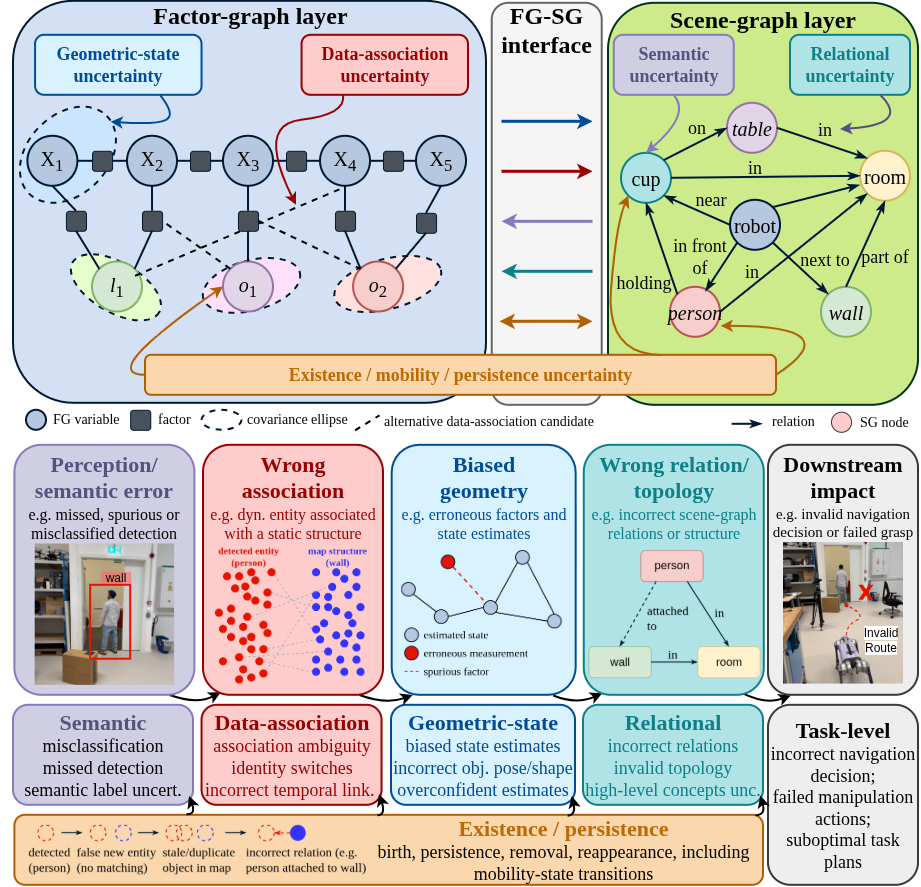
\includegraphics[width=0.99\columnwidth]{Figures/figure_FG_SG_uncertainty_boundary_new_final.png}
    \caption{Uncertainty types and their interface in hybrid factor graph-scene graph world models.}
    \label{fig:FG_SG_uncertainty_boundary}
\end{figure}


%% Uncertainty propagation across the FG-SG boundary
\subsubsection{Uncertainty Types, Propagation, Failure Modes, and Scalability}\label{sec:uncertainty_types}
Uncertainty in graph-based world models does not constitute a single interchangeable quantity, but arises over different latent variables and decisions throughout the representation pipeline.
We distinguish five uncertainty classes that recur across the surveyed approaches: (i) \textit{geometric-state uncertainty}, concerning continuous quantities such as robot poses, landmark positions, object poses, and motion; (ii) \textit{semantic uncertainty}, concerning class labels, attributes, or other learned semantic predictions; (iii) \textit{data-association uncertainty}, concerning which observation corresponds to which existing entity; (iv) \textit{existence uncertainty}, concerning whether an entity is present, persists, disappeared, or should be instantiated; and (v) \textit{relational uncertainty}, concerning the validity of scene-graph edges between entities. 
These uncertainty classes characterize the uncertain quantities or hypotheses represented by the world model and should be distinguished from the sources of uncertainty entering the inference process. 
For geometric estimation in particular, sensor and odometry noise appear as measurement uncertainty on observation factors, while imperfect motion or structural assumptions introduce model uncertainty through prior factors. 
Both contribute to the posterior uncertainty of geometric state variables.
These uncertainty classes differ both in their mathematical representation and in how they propagate through the world model.
Consequently, a system can provide a principled probabilistic treatment for one class while treating others deterministically or through heuristic confidence measures.

\begin{table*}[t]
\centering
\caption{Uncertainty classes in graph-based dynamic world models.}
\label{tab:uncertainty_classes}
\renewcommand{\arraystretch}{1.15}
\setlength{\tabcolsep}{4pt}
\scriptsize
\begin{tabularx}{\textwidth}{
    >{\raggedright\arraybackslash}p{0.07\textwidth}
    >{\raggedright\arraybackslash}p{0.16\textwidth}
    >{\raggedright\arraybackslash}p{0.23\textwidth}
    >{\raggedright\arraybackslash}p{0.23\textwidth}
    >{\raggedright\arraybackslash}X}
\hline
\textbf{Uncertainty class} &
\textbf{Uncertain quantity} &
\textbf{Typical representation / treatment} &
\textbf{Representative mechanisms} &
\textbf{Main cross-layer issue} \\
\hline

Geometric state &
Robot/object pose, landmark position, velocity motion &
Measurement/odometry factor noise models; motion-prior/model covariance; posterior state covariance or information &
Probabilistic factor-graph estimation and smoothing; marginal covariance estimation; adaptive or learned factor covariance &
Propagation from geometric states to scene-graph entities and relations \\

Semantic &
Class labels, attributes, semantic observations &
Learned class probabilities or confidence measures; uncertainty-weighted semantic factors &
Semantic perception; learned semantic factor uncertainty &
Calibration and transfer of perception uncertainty into probabilistic estimation \\

Data association &
Observation-to-entity correspondence &
Discrete hypotheses, association probabilities, latent or switchable variables &
JPDA, MHT, weighted or switchable constraints &
Incorrect associations alter graph structure and cannot be represented by state covariance alone \\

Existence &
Entity presence, persistence, birth, and removal &
Bernoulli existence probability; Random Finite Set intensities and mixtures &
Bernoulli, PHD, and PMBM filtering; persistence and decay models &
Coupling probabilistic birth/death estimates to scene-graph node lifecycle \\

Relational &
Validity of scene-graph edges or predicates &
Learned probabilities or heuristic confidence measures; often deterministic &
Spatial, semantic, and functional relation inference &
Propagation of endpoint-state and semantic uncertainty into relation confidence \\

\hline
\end{tabularx}
\end{table*}


These uncertainty classes, summarized in Table \ref{tab:uncertainty_classes}, interact but cannot generally be propagated using the same mechanism. 
Geometric-state uncertainty is continuous and naturally represented within factor-graph inference, whereas data association and existence involve discrete hypotheses or latent variables. 
Semantic uncertainty originates primarily from learned perception and may influence factor weights or association decisions, while relational uncertainty concerns higher-level graph structure.
Errors can therefore propagate across classes: uncertain semantics may induce an incorrect association, an incorrect association may bias geometric estimation, uncertain existence may trigger premature node deletion, and uncertain endpoint states may invalidate a scene-graph relation. 
A central limitation of current hybrid FG-SG systems is that these cross-class dependencies are rarely represented within a single probabilistic model.

Across the surveyed systems, these five classes exhibit markedly different degrees of explicit probabilistic treatment. Geometric-state uncertainty is the most systematically represented: factor-graph-based approaches routinely associate measurement and prior factors with covariance or information models and propagate their effect through state estimation.
Semantic uncertainty is less consistently preserved: learned perception front-ends often provide class probabilities or confidence scores, but these are frequently converted into deterministic labels before entering the world model or used only to modulate selected factor weights.
Data association uncertainty is similarly heterogeneous: although probabilistic multi-hypothesis formulations such as JPDA and MHT provide explicit distributions over correspondences, many practical systems commit to deterministic geometric, appearance, or learned-similarity matches. 
Existence uncertainty is generally handled through persistence scores, decay rules, or geometric verification, while explicit Bernoulli/RFS-based existence probabilities remain uncommon in integrated FG-SG systems. 
Relational uncertainty is the least developed class: scene-graph predicates are commonly instantiated deterministically or accompanied by learned confidence scores, with little explicit propagation of uncertainty from their endpoint states.
The uncertainty profiles reported in Table \ref{tab:taxonomy_overview} reflect this imbalance, with probabilistic treatment concentrated primarily in geometric estimation and substantially weaker probabilistic support toward semantic and relational layers.

The consequences of neglecting these uncertainty classes are also different. 
Mischaracterized measurement or motion-model uncertainty changes the weighting of geometric factors and can produce overconfident or biased state estimates.
Incorrectly calibrated semantic confidence may alter factor weighting or association decisions.
Data-association errors are more severe structurally. Once an observation is assigned to the wrong entity, a small conditional pose covariance does not represent the uncertainty of that assignment. Poor existence modeling produces either stale entities or premature deletion, while overconfident relational inference can propagate uncertain geometric or semantic states into incorrect high-level graph edges consumed by planning and reasoning.
These failure modes therefore cannot be diagnosed or mitigated through geometric covariance alone.

Geometric-state uncertainty is the most mature of these classes within factor-graph formulations. Measurement factors, including sensor observations and odometry constraints, encode measurement uncertainty through noise models, covariance matrices, or information matrices.
Motion-prior factors similarly encode uncertainty associated with the assumed evolution model.
These uncertainties are fused through probabilistic inference, and posterior marginal state covariances can be obtained from the resulting joint information matrix, commonly using a local Gaussian approximation around the MAP estimate \cite{dellaert_factor_2017}.
\textcolor{red}{The difficulty arises at the boundary: how does the uncertainty of the pose nodes in a factor graph propagate into the semantic and relational claims made by a scene graph node?
In the layered-stack architecture, this propagation is largely absent, as shown in Figure \ref{fig:FG_SG_uncertainty_boundary}.
Scene graph nodes that are instantiated from a poorly constrained region of the pose graph  carry the same confidence as one from a well constrained area. 
In dynamic settings, where uncertainty is generally higher and crucial for spatio-temporal estimation and prediction, this is a large drawback.
Systems that adopt the unified optimizable graph architecture handle this more naturally: by representing semantic entities as factor graph variables, their states participate in the joint information structure, allowing their posterior uncertainty to reflect the geometric and semantic constraints included in the optimization \cite{bavle_s-graphs_2025}.}
\hl{At the FG-SG interface, it is important to distinguish uncertainty representation from uncertainty propagation. 
The former concerns which uncertainty quantities are explicitly modeled, whereas the latter concerns how their uncertainty affects estimates or beliefs in another representation.
In a layered architecture, geometric-state uncertainty can be propagated forward by transferring state distribution, marginal covariances, or appropriate approximations alongside the optimized geometric states. This does not require semantic feedback to the factor graph.

However, when only point estimates or deterministic labels are transferred, information about uncertainty and correlations may be lost at the interface. Even when marginal covariances are retained, dependencies between entities may be discarded, limiting the subsequent assessment of relational uncertainty. 

In unified optimizable graph architectures, the geometric states of semantic entities participate directly in the joint estimation problem, as in S-Graphs} \cite{bavle_s-graphs_2025}. \hl{This allows their posterior uncertainty to reflect the dependencies encoded by the included factors.
Nevertheless, joint MAP estimation does not imply that posterior covariances are explicitly recovered, nor that uncertainty over semantic labels, entity existence, or scene-graph relations is represented probabilistically.}
\hl{For example, consider the relative position between two scene-graph entities, $\mathbf{d_{ij}} = \mathbf{p_i} - \mathbf{p_j}$. Its covariance is given by:}
\begin{equation}
    \Sigma_{d_{ij}} = \Sigma_{ii} + \Sigma_{jj} - \Sigma_{ij} - \Sigma_{ji}
\end{equation}
\hl{where $\Sigma_{ii}$ and $\Sigma_{jj}$ denote the marginal position covariances, and $\Sigma_{ij}$ and $\Sigma_{ji}$ their cross-covariances. Transferring only individual state estimates or marginal covariances may therefore be insufficient to correctly characterize the uncertainty of a spatial relation. This illustrates that the preservation of statistical dependencies across representation layers is distinct from the direction of information flow.}
\hl{Existing systems demonstrate different aspects of uncertainty handling rather than a complete cross-representation propagation mechanism. For instance, Kimera} \cite{rosinol_kimera_2021} \hl{ and Hydra }\cite{hughes_hydra_2022} \hl{perform Bayesian fusion of semantic observation at the voxel level, but this is distinct from propagating geometric posterior uncertainty into scene-graph relations. Similarly, the joint estimation of geometric states associated with semantic entities in S-Graphs does not by itself provide probabilistic beliefs over all semantic and relational attributes.}
Recent work by Millan-Romera et al. \cite{millanromera2026generationuncertaintyawarehighlevelspatial} demonstrates that incorporating learned uncertainty estimates for semantic factors, rather than fixed information matrices, further improves SLAM accuracy, particularly in edge cases where semantic concepts are the only cues preserving geometric consistency.

A poorly-constrained dynamic entity node produces an unreliable trajectory estimate that, if allowed to influence loop-closure candidates, can corrupt the static map, too\cite{giberna_dynemo-slam_2025}.
%Khronos \cite{schmid_khronos_2024} addresses this through explicit 4D metric uncertainty on object fragments, distinguishing reliable observations from transient ones before any graph level update is triggered. 
Khronos \cite{schmid_khronos_2024} mitigates this by \textcolor{red}{attaching explicit 4D metric uncertainty to its object fragments before they are committed to the global graph, rather than treating every instantiated node as equally confident.} \hl{aggregating locally consistent observations into object fragments, jointly optimizing fragment positions and robot poses using robust geometric constraints, and performing geometric verification before reconciling fragments into persistent objects. 
These mechanisms improve the robustness of the resulting representation, but do not constitute explicit propagation of posterior geometric uncertainty into higher-level semantic relations.} 
The broader challenge, i.e., consistent propagation of geometric and temporal uncertainty into semantic relations, (e.g., how certain is the \textit{on} edge between an object and a table, given the covariance on both their pose nodes?) remains largely open and represents one of the key research gaps identified in Section \ref{sec:challenges_future_works}.

A related failure mode in dynamic environments is the corruption of higher-level scene graph abstractions by incorrect dynamic entity handling. 
If a moving person is incorrectly associated with a static wall node during a period of high dynamics, the resulting factor introduces a misleading constraint into the joint optimization that can displace the wall node and corrupt the room topology built on top. 
This cross-layer error propagation is difficult to detect and correct a posteriori, motivating the use of explicit confidence gating to prevent semantically inconsistent observations from entering the graph \cite{zhang_outlier_2023}.
Viewed end-to-end, these errors form a propagation chain rather than isolated module failures. 
A missed or incorrect detection can create a missing or misclassified entity, an incorrect association can lead to an erroneous factor and bias the estimated state, biased states can in turn affect scene-graph relations or topology. 
Downstream modules then consume this corrupted representation, so an incorrect relation or object state may ultimately produce an invalid navigation decision or manipulation task. 
Robust complete systems therefore require uncertainty and consistency checks across the interfaces between perception, estimation, abstraction and action, rather than only within individual modules.
Importantly, errors are not propagated uniformly across this chain.
Continuous measurement errors may be attenuated through repeated observations, robust factor weighting, and joint optimization, whereas discrete errors such as incorrect identity association, false entity instantiation, or premature deletion can alter the graph structure itself and persist across subsequent updates.
The interfaces between perception, association, estimation, and abstraction therefore act either as error filters or error-amplification points.
Temporal aggregation and robust estimation can suppress noisy observations before they affect the persistent model, while an incorrect committed association can create a structurally valid but semantically wrong factor that subsequently biases geometric states and higher-level relations.

%% computation scalability
The trade-off between representational richness and real-time inference is a challenge for hybrid factor graph-scene graph systems.
As the environment grows, both the factor graph and the scene graph accumulate nodes and edges, and the computational cost of optimization scales with graph density.
Several strategies have been developed to manage this.
\textit{Hierarchical optimization} exploits the layered structure of scene graphs to scope optimization to the relevant subgraph: S-Graphs 2.0 \cite{bavle_s-graphs_2025} runs room-level local optimization continuously and floor-level global optimization only on loop closure, avoiding full re-optimization of the entire graph at each update.
\textit{Marginalization and sparsification} are applied at the factor graph layer to maintain a bounded-size active window, with older variables marginalized into prior factors. 
DynoSAM \cite{morris_dynosam_2025} and its hybrid world-object centric formulation \cite{morris_online_2025} use embedded-frame anchoring (Section \ref{sec:construction_pipeline_backend}) to preserve sparsity as dynamic object maps grow.
\textit{Task-driven graph pruning}, detailed in Section \ref{sec:querying_reasoning_action_action}, reduces the relational superstructure to a minimal actionable subgraph relevant to the current task, as in Clio \cite{maggio_clio_2024} and SayPlan \cite{rana2023sayplangroundinglargelanguage}, preventing the planning complexity from growing with the full map. 
Together these strategies allow hybrid systems like Khronos \cite{schmid_khronos_2024} and DynEMo-SLAM \cite{giberna_dynemo-slam_2025} to achieve real-time performance in complex large indoor environments. However, the scalability of unified optimizable graphs to large-scale, highly dynamic outdoor scenes where both the agent population and the structural complexity are greater, remains an active research direction and will be discussed in more detail in Section \ref{sec:construction_pipeline_backend}.




% The literature converges on a hierarchical layer stack where the factor graph explicitly grounds the scene graph nodes in a shared spatial reference frame. 
% This leads to having at the base \textbf{the Geometric Foundation}, a metric semantic mesh/point cloud which provides spatial grounding \cite{rosinol_3d_2020}. This layer is frequently maintained by factor graph optimizers, which simultaneously optimze the robot's trajectory and the mesh vertices or point cloud during loop closures to maintain global consistency. 
% Next, the \textbf{Object-Agent Layer} follows, categorizing entities into generally-static objects and time-varying agents. In dynamic settings, agents are represented as secondary pose graphs within the factor graph, capturing their trajectories as sequences of time-stamped pose variables \cite{giberna_dynemo-slam_2025}.
% On top, the \textbf{Relational Superstructure} contains topology nodes that are connected to the underlying metric landmarks through inter-layer edges, allowing high-level reasoning such as resolving queries like "which objects are in this rooms" or "which objects is next to this one" while maintaining the geometric precision needed for navigation. 

Figure \ref{fig:unifying_view_SG_FG} summarizes this hybrid architecture, showing how the factor graph backbone and scene graph superstructure connect through shared dynamic modeling and graph-maintenance stages to support downstream querying, reasoning and action.
This unified representation enables actionable spatial perception, where the world model is not merely a passive map but a persistent, query-able substrate for planning, interaction, and scene prediction.

\begin{figure}
    \centering
    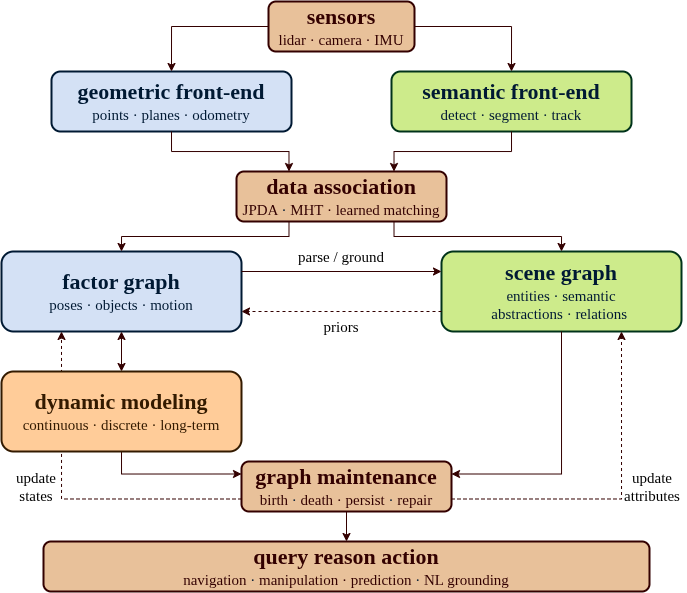
\includegraphics[width=\columnwidth]{Figures/figure_FG_SG_architecture.png}
    \caption{Conceptual architecture of a hybrid probabilistic graph-based dynamic world model.}
    \label{fig:unifying_view_SG_FG}
\end{figure}

\subsection{Representing Dynamics in Graph-Based World Models}\label{sec:dynamics_representations}
The evolution of world model representations for robotics in non-stationary scenarios has progressed from treating environmental change as outlier noise toward a systematic, relational and probabilistic characterization of dynamics across multiple temporal scales \cite{rosinol_3d_2020} \cite{schmid_khronos_2024}.
This section presents the most common characterization of dynamic entities in dynamic world modeling. Specifically, we emphasize the integration of factor graphs and 3DSGs to handle short-term dynamics (Section \ref{sec:dynamics_representations_agents}), semi-static changes (Section \ref{sec:dynamics_representations_objects}), and long-term structural evolution (Section \ref{sec:dynamics_representations_longterm}). 
Figure \ref{fig:dynamics_timescale} depicts the dynamic distinction we adopt \textcolor{red}{, based on the type and temporal scale of expected motion}, highlighting \hl{typical but non-defining temporal ranges and} some relevant works focusing on each of them.

\begin{figure}[!ht]
    \centering
    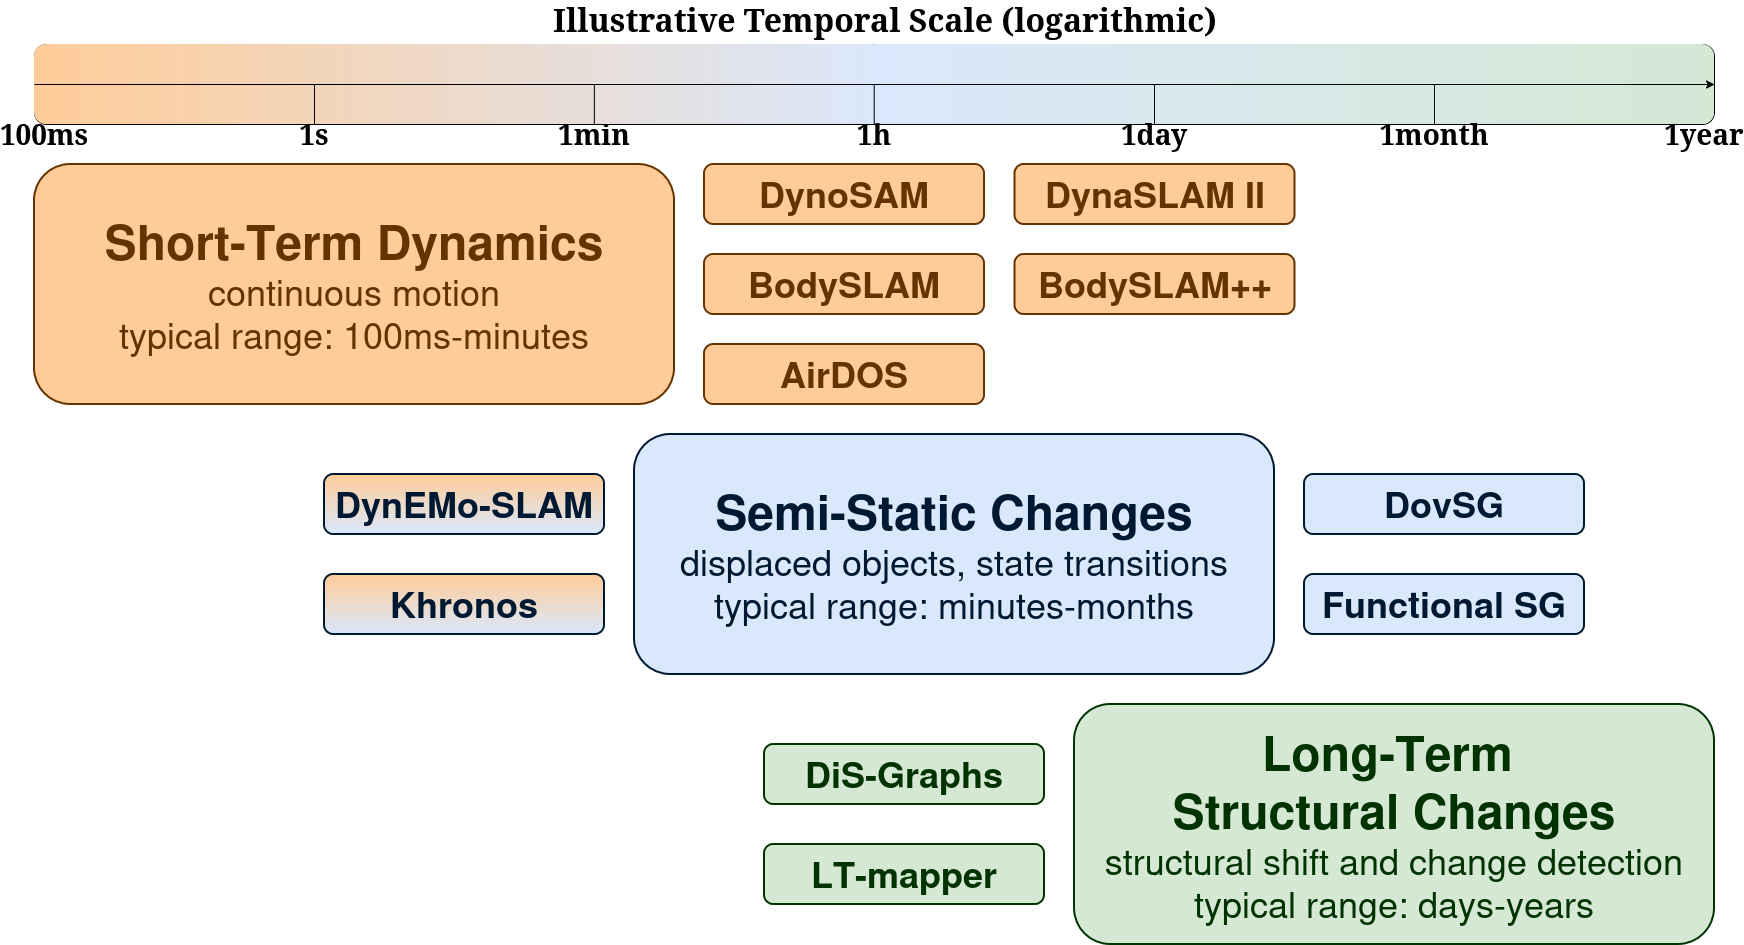
\includegraphics[width=0.9\columnwidth]{Figures/figure_dynamics_timescale_updated.png}
    \caption{Diagram showing the adopted  temporal-horizon taxonomy. \hl{The reported temporal ranges are indicative of typical timescales and do not constitute fixed classification boundaries.} The tiers denote operational change regimes \hl{relative to the robot's observation and wold model update horizons,} rather than mutually exclusive entity classes\textcolor{red}{, t} \hl{. T}he same entity or system may span multiple tiers. Relevant works are reported for each, or group of, type of dynamics.}
    \label{fig:dynamics_timescale}
\end{figure}


\subsubsection{Short-Term Dynamics}\label{sec:dynamics_representations_agents}
In an environment populated by humans and/or moving objects, the world model must resolve the ``motion ambiguity'' where pixel or point displacement is a compound effect of the simultaneous robot's ego motion and the independent motion of other entities \cite{zhang_semantic-integrated_2026}. 

%% Separate static Map vs Dynamic Layer (Loosely coupled SLAMMOT)
Early paradigms typically treated short-term dynamic entities as outliers to be masked or rejected \cite{bescos_dynaslam_2018} to preserve the consistency of a purely static map. 
Contemporary loosely coupled systems often maintain these as separate threads, using the camera pose as a prior for multi object tracking (MOT) but without allowing object measurements to refine the ego-localization\cite{tian_dl-slot_2024} \textcolor{red}{\cite{tian_dl-slot_2024}} \cite{gou_visual_2024}. 
In this way, a uni-directional flow of information is generated, allowing the optimized static map data, output of the SLAM process, to enhance MOT but not the other way around.

%% Fully Coupled Joint optimization frameworks
Modern representations employ a tightly-coupled SLAMMOT approach, where the factor graph back-end jointly optimizes camera poses, static landmarks, and the trajectories of dynamic objects or agents within a unified optimization manifold \cite{zhang_semantic-integrated_2026}.
Systems like DynaSLAM II \cite{bescos_dynaslam_2021}, DynEMo-SLAM \cite{giberna_dynemo-slam_2025}, SMMF-SLAMMOT \cite{zhang_semantic-integrated_2026} support a tightly-coupled approach where robot poses, static landmarks, and dynamic entity trajectories are jointly optimized in a unified factor graph.
This paradigm requires spatio-temporal reprojection factors to introduce cross-terms between camera poses and object motions, ensuring that the estimation of self and the surrounding is mutually beneficial. 
% employ spatio-temporal reprojection factors that couple geometric observations across frames to enforce rigid-body kinematic constraints, effectively improving both self-localization and object tracking accuracy. 
%% Hybrid Efficiency 
To address the computational effort of joint optimization, DynoSAM\cite{morris_dynosam_2025} and Hybrid iSAM2 \cite{morris_online_2025} formulations anchor rigid body motions to ``embedded frames'', preserving graph sparsity as each object map grows while enabling efficient incremental inference by a Bayes Tree. 
% This allows each object map to grow as new fragments become visible while preserving graph sparsity, enabling efficient incremental inference via the Bayes Tree.

%% Coordinate frame representation (MOVED to VI-A)
% A critical design choice involves the coordinate frames used for agents states. 
% While object-centric formulations express points in a local body frame to enforce rigidity, recent analysis indicates that world-centric or hybrid representations, which anchor motions to an "embedded frame" established at the first observation, superiorly preserve factor graph sparsity and enhance solver efficiency for incremental optimizers like iSAM2 \cite{morris_importance_2024} \cite{morris_online_2025}.

%% Agent specific states
% Humans are often represented with specific node types containing 3D pose graphs for their trajectories and non-rigid shape models, such as Skinned Multi-Person Linear Model (SMPL) meshes \cite{loper_smpl_2015}, ensuring the world model accounts for both articulated motion and volumetric presence \cite{rosinol_kimera_2021} \cite{schmid_khronos_2024}.
% TODO go deeper in SMPL, bodyslam and bodyslam++ and other human models
Humans represent a particularly important and challenging sub-class of short-term dynamics, often referred to as \textit{dynamic agents}: they are simultaneously the most common source of dynamics in real-world environments and the most structurally complex entity to model. This stems from the fact that humans fall into the challenging \textit{articulated} and \textit{goal-driven} categories along the typology and behavioral intent axes, respectively.
Systems like Kimera \cite{rosinol_kimera_2021} and Khronos \cite{schmid_khronos_2024} represent humans with dedicated node types combining 3D pose graph trajectories with non-rigid models, ensuring the world models account for both articulated motion and volumetric presence. 
BodySLAM \cite{henning_bodyslam_2022} and its successor BodySLAM++ \cite{henning_bodyslam_2023} push this further, pioneering the joint optimization of camera trajectory and dense human body shape and pose within a single factor graph, where each human observation is a parametric body model linked to the camera pose graph via reprojection factors. 
BodySLAM++ \cite{henning_bodyslam_2023} extends this to multiple simultaneous human instances, integrating inertial factors in a real-time fashion, improving robustness to occlusion in crowded scenes. 
In both cases, the structured prior provided by the body model regularizes an otherwise underconstrained problem, the same role played by rigid-body kinematic priors for object-class short-term dynamics, like for instance in \cite{qiu2022airdos} accounting for dynamic articulated objects.

%% human body models
The choice of the body model determines the degrees of freedom exposed to the optimizer and the computational costs of inference. 
Parametric models dominate in SLAM-integrated systems: SMPL \cite{loper_smpl_2015} represents the body as a compact, differentiable parameter vector via linear blend skinning, making it naturally compatible with factor graph optimization \cite{henning_bodyslam_2022}\cite{henning_bodyslam_2023}.
SMPL-X \cite{SMPL-X:2019} extends this to hands and face, while STAR \cite{STAR:2020} reduces blend skinning artifacts at extreme poses. 
For monocular initialization without depth sensors,  learned estimators such as VIBE \cite{kocabas2019vibe}, FrankMocap \cite{rong2021frankmocap}\cite{joo2020eft} and PromptHMR \cite{wang2025prompthmr} provide  body-model parameters. 
At the opposite end,  METRO \cite{lin2021end-to-end} directly predicts mesh vertices, while  InstantAvatar \cite{jiang2022instantavatar}  learns a subject-specific neural representation. These approaches replace the compact fixed-dimensional parameterization of SMPL-family models with higher-dimensional representations that are less directly suited to integration as factor-graph state variables. 
The prevailing trade-off is therefore between the structured compactness of SMPL-family models and the expressiveness of learned representations, summarized in Table~\ref{tab:body_models}.

\begin{table*}[t]
\centering
\caption{Comparison of human body representations and inference methods relevant to robotic world modeling.}
\label{tab:body_models}
\resizebox{\textwidth}{!}{
\begin{tabular}{llllllll}
\toprule
\textbf{Model} & \textbf{Input} & \textcolor{yellow}{\textbf{Method Type}} & \textbf{Hardware} & \textbf{Training} & \textbf{Output} & \textbf{Body Parts} & \textbf{Use Case} \\
\midrule

SMPL \cite{loper_smpl_2015}
& Shape/pose params
& Parametric body model
& CPU/GPU
& Offline (scan-based)
& Parametric mesh
& Body only
& SLAM, MOT, animation \\

SMPL-X \cite{SMPL-X:2019}
& Shape/pose/expr.\ params
& Parametric expressive body model
& GPU
& Offline (scan-based)
& Parametric mesh
& Body + hands + face
& Expressive HRI, animation \\

STAR \cite{STAR:2020}
& Shape/pose params
& Parametric body model
& CPU/GPU
& Offline (scan-based)
& Parametric mesh
& Body only
& SLAM, extreme pose recovery \\

Anny \cite{bregier2025humanmeshmodelinganny}
& Phenotype params
& Parametric phenotype-conditioned body model
& CPU/GPU
& None (scan-free)
& Parametric mesh
& Body + hands + face
& Diverse pop.\ modeling, HMR \\

VIBE \cite{kocabas2019vibe}
& Monocular video
& Temporal SMPL regressor
& GPU
& Offline (video data)
& SMPL params/frame
& Body only
& Video-based pose init. \\

FrankMocap \cite{rong2021frankmocap} \cite{joo2020eft}
& RGB image
& Whole body regressor + integration
& GPU
& Offline (images)
& SMPL-X params
& Body + hands
& Real-time monocular HMR \\

METRO \cite{lin2021end-to-end}
& RGB image
& Direct mesh regressor
& GPU (high-end)
& Offline (images)
& Raw mesh vertices
& Body + hands
& Accurate shape recovery \\

PromptHMR \cite{wang2025prompthmr} &
RGB image + spatial/semantic prompts &
Prompt-conditioned mesh regressor &
GPU &
Offline &
SMPL-X parameters &
Body + hands + face &
Promptable multi-person HMR / interaction \\

InstantAvatar \cite{jiang2022instantavatar}
& Monocular video
& Subject-specific neural avatar
& GPU (high-end)
& Per-subject online
& Neural field + mesh
& Full body
& Avatar reconstruction \\

\bottomrule
\end{tabular}
}
\end{table*}

% e.g. moving humans, moving objects... 
% Joint SLAM+tracking: objects nodes have state over time.
% Key question: separate static map vs dynamic layer, or fully coupled?

\subsubsection{Semi-Static Changes}\label{sec:dynamics_representations_objects}
Semi-static dynamics involve objects that are stationary during observation but relocated over time, ending up displaced in future observations \cite{brink_using_2016} \cite{giberna_dynemo-slam_2025}.
This requires the model to distinguish between ``moving'' and ``movable'' states. 
Additionally, it is needed to learn what kinds of changes a specific entity can undergo and how to handle object disappearance. 

%% State variables and changes and Affordances
Nodes in modern 3DSGs are annotated with dynamic attributes such as \textit{open/closed} or \textit{on/off} \cite{olivastri_multi-modal_2024}. 
These properties, often inferred via Vision-Language Models \cite{shao_large_2025}, define \textit{functional scene graphs} \cite{rotondi_fungraph_2025} \cite{zhang_open-vocabulary_2025} where interactive elements like handles are linked to the objects they trigger, ending up to change their states. 

%% Object Permanence vs Forgetting
The key question of permanence is handled via hierarchy and containment edges (for instance an object in a drawer) \cite{behrens_lost_2025} \cite{yan_dynamic_2025}.
Systems like Lost \& Found \cite{behrens_lost_2025} maintain object permanence by updating these relations online. 
If a human hides an item in a drawer, the \textit{contains} edge ensures the robot \textit{remembers} the location despite total occlusion. 

%% Inactive Nodes vs delation
Decisions to prune the graph are often governed by probabilistic decay rates \cite{gomez_object-based_2020} or explicit geometric verification \cite{schmid_khronos_2024}.
In DPG-SLAM \cite{walcott-bryant_dynamic_2012}, sectors of a node are turned off if they intersect with evidence of removal. 
A node is marked inactive if a threshold of sectors is off, but it is only deleted if it no longer provides useful topological information, thereby managing complexity without losing historical data. 
% e.g. moved objects, changed states
% add state variable (open/closed) and persistence logic.
% Key Question: object permanence vs forgetting: when do nodes get deleted vs marked inactive.

\subsubsection{Long-Term Structural Changes} \label{sec:dynamics_representations_longterm}
Lifelong autonomy necessitates a world model that can align multiple sessions and detect structural shifts in the environment \cite{deeb_model-based_2019} \cite{catalano_3d_2025}, precluding the assumption of staticity in entities or parts of the map which would otherwise be considered unmovable in shorter or single-session campaigns.

%% structural change detection
At geometric level, structural change detection compares observations from different sessions to classify map regions as stable, changed or newly appeared. 
DPG-SLAM \cite{walcott-bryant_dynamic_2012} addresses this by continuously comparing current sensor data against submaps from previous sessions.
Regions where contradictions occur are marked as changed, and associated nodes are pruned.
LT-mapper \cite{kim2022lt} extends this to large-scale outdoor LiDAR SLAM through anchor-node-based inter-session loop factors that align drifted session pose graphs into a shared coordinate frame, applying then set-difference operations to identify positive and negative changes at keyframe level.
% Khronos \cite{schmid_khronos_2024} handles this through its spatio-temporal factorization. 
% The asynchronous global process continuously checks the current metric-semantic mesh against the accumulated map, triggering node deactivation when ray-tracing evidence confirms structural removal.

%% multi-session aligment  and graph updates
Merging observations from multiple sessions into a globally consistent factor graph requires solving both the inter-session pose offset and the data association between observation of potentially changed structures.
The standard mechanism is the introduction of inter-session loop closure factors, i.e.,  constraints between nodes from different sessions that share stable landmarks \cite{kim2022lt}.
Memory management is critical to keep this tractable. As shown in \cite{labbe2014online}, a hierarchical short-term/working/long-term memory structure can bound the number of loop closure candidates, enabling multi-session operation under computational constraints. 

%% structural priors
A complementary approach to multi-session alignment uses prior structural knowledge, typically in form of Building Information Models (BIM) or architectural plans, to anchor the factor graph to a known coordinate frame and constrain the estimation of structural elements. 
BIM-SLAM \cite{vega_torres_bim-slam_2023} models both the robot's SLAM graph and the architectural plan as a hierarchical factor graph, then detects inter-session loop closure between them. 
DiS-Graphs \cite{shaheer_tightly_2025} extends this to jointly estimate deviations between the planned and the built environments, incorporating BIM-derived structural priors as soft constraints in the factor graph to remain accurate even when the real building deviates from its original plans.
The key insight in both works lies in the hierarchical scene graph structure, e.g., walls, rooms, floors, which provides a natural alignment target that is more robust to partial scene change than point-level descriptors.
The graph update policy in these systems therefore distinguishes between permanent structural entities, even in cases of deviations or changes, which are retained and used for inter-session alignment, and semi-static or movable entities.

%\input{Sections/dynamics_types}
%% How to create it
\section{Dynamic World Model Construction}\label{sec:construction_pipeline}
Dynamic world model construction refers to the end-to-end process by which raw sensor observations are transformed into a persistent, probabilistically grounded, and semantically structured representation of a non-stationary environment. 
In hybrid representations combining factor graphs and scene graphs, this process spans multiple tightly interacting stages, from front-end perception and data association to back-end inference and long-term graph maintenance.

Rather than a monolithic pipeline, modern systems adopt modular yet interdependent components, where design choices at early stages (e.g., detection granularity or association strategy) strongly influence the stability, scalability, and expressiveness of the resulting world model under dynamics.
This section organizes existing approaches around four core stages that recur across the literature: front-end perception (Section \ref{sec:construction_pipeline_frontend}), data association (Section \ref{sec:construction_pipeline_data_association}), back-end inference and optimization (Section \ref{sec:construction_pipeline_backend}), and graph maintenance (Section \ref{sec:construction_pipeline_graph_maintenance}).
A general pipeline overview is depicted in Figure \ref{fig:FG_SG_world_model_construction_maintenance_workflow}.

\subsection{Front-End Perception}\label{sec:construction_pipeline_frontend}
The front-end perception stage is responsible for extracting candidate entities, attributes and relations from raw sensor data.
In dynamic environments, this stage must operate under partial observability, occlusion and motion ambiguity, while providing sufficiently rich primitives for downstream probabilistic inference. 

\subsubsection{Geometric and Semantic Primitives}
At the geometric level, front-ends extract low-level features such as points, lines, planes or surfels, which remain the backbone of factor graph-based SLAM systems \cite{dellaert_factor_2017} \cite{rosinol_kimera_2021}. 
However, dynamic scenes increasingly require object- and agent-level primitives, motivating the integration of instance segmentation, 3D bounding volumes, or parametric object models \cite{bescos_dynaslam_2021} \cite{morris_dynosam_2025} \cite{schmid_khronos_2024}.

Semantic perception pipelines typically produce:
\begin{itemize}
    \item \textbf{Object detections and instances}, often class-labeled and possibly open-vocabulary \cite{yan_dynamic_2025} \cite{gu_conceptgraphs_2023};
    \item \textbf{Agent hypotheses}, including humans or vehicles, sometimes with articulated or rigid-body structure \cite{henning_bodyslam_2022} \cite{qiu2022airdos};
    \item \textbf{Attribute estimates}, such as object state (open/close, on/off) \cite{olivastri_multi-modal_2024};
    \item \textbf{Relation hypotheses}, e.g., spatial (on, in, next-to) or functional (controls, supports) \cite{catalano_3d_2025} \cite{zhang_open-vocabulary_2025}.
\end{itemize}

In hybrid FG-SG systems like Kimera \cite{rosinol_kimera_2021} or Khronos \cite{schmid_khronos_2024}, these outputs are deliberately redundant: dense geometric observations coexist with higher-level semantic abstraction, resulting in robustness to perception failures. 

\subsubsection{Temporal Grouping and Tracking}
To cope with dynamics, front-ends often incorporate \textit{short-term temporal aggregation}, producing tracklets or object fragments prior to global optimization. 
Optical flow, frame-to-frame association, or local tracking modules are commonly used to stabilize detections before they enter the global world model \cite{morris_dynosam_2025} \cite{schmid_khronos_2024}.
Khronos \cite{schmid_khronos_2024}, for example, explicitly constructs temporally consistent object fragments ahead of the active-window integration described in Section \ref{sec:dyn_world_model_representations_scene_graphs}, postponing commitment to the global model until sufficient evidence is accumulated.

This early temporal coherence reduces spurious node creation and limits the combinatorial computational effort on later data association stages.
From an end-to-end perspective, these front-end mechanisms constitute the first error-containment stage of the world-model pipeline: temporal aggregation can suppress isolated false detections or noisy estimates before they become persistent graph entities.
Conversely, systematic missed detections or misclassifications that survive this stage are passed to association and graph construction, where they may become persistent structural errors.

\subsection{Data Association}\label{sec:construction_pipeline_data_association}
Data association is the process of determining which observations correspond to which existing entities in the world model, or whether they should instantiate new ones. 
In dynamic environments, association errors are among the primary failure reasons, as incorrect correspondences can propagate across time,  corrupting both geometric estimation and semantic structure. 

\subsubsection{Deterministic and Probabilistic Association}
Classical SLAM systems rely on deterministic association mechanisms, such as nearest-neighbor matching or Hungarian assignment based on geometric or appearance similarity \cite{lingzhu_xiang_robust_2015} \cite{gou_visual_2024}. 
While efficient, these approaches degrade quickly under occlusion and fast motion.

To address this, many dynamic-world-model systems employ \textit{probabilistic multi-hypothesis association}, including:
\begin{itemize}
    \item \textbf{Joint Probabilistic Data Association (JPDA)}, which marginalizes over multiple correspondence hypotheses \cite{gulati_robust_2017};
    \item \textbf{Multiple Hypothesis Tracking (MHT)}, which explicitly maintains competing association trees over time \cite{zaech_learnable_2022};
    \item \textbf{Learned association}, where neural embeddings (e.g. CLIP features) define similarity metrics for object re-identification \cite{gu_conceptgraphs_2023} \cite{yan_dynamic_2025}.
\end{itemize}
In factor-graph formulations, association decisions are often represented implicitly via latent correspondence variables or explicitly through switchable or weighted constraints \cite{giberna_dynemo-slam_2025} \cite{lingzhu_xiang_robust_2015}.
This association uncertainty is distinct from geometric-state uncertainty. A small pose covariance conditioned on an incorrect correspondence does not imply that the correspondence itself is reliable, motivating explicit treatment of competing association hypotheses.

Data association is therefore a particularly critical propagation interface.
Unlike continuous measurement noise, which often can be reduced by additional observations, committing an observation to the wrong entity changes which states are connected by subsequent factors and may contaminate both the estimated geometry and the semantic history of that entity.

\subsubsection{Association under Dynamics}
Dynamic environments need distinguishing between moving agents, movable but stationary objects, and ephemeral observations, like transient clutter or false positives.
Several works incorporate \textit{movability or existence variables} to mediate association decisions \cite{brink_using_2016} \cite{gomez_object-based_2020}.  
From a probabilistic perspective, Random Finite Set (RFS)-based formulations (Section \ref{sec:construction_pipeline_graph_maintenance}) provide a mechanism for handling association, birth and death jointly \cite{ristic2013tutorial} \cite{garcia2018poisson}, although full integration with scene graph construction remains limited.
Open-vocabulary embeddings extend data association beyond predefined semantic classes, but they primarily provide semantic generality rather than a probabilistic association model. 
Their similarity scores should therefore not be interpreted as equivalent to posterior association probabilities produced by multi-hypothesis methods such as JPDA or MHT. This distinction becomes particularly important under dynamics, where visually similar objects, occlusion, and viewpoint change can produce confident but incorrect semantic matches.

\subsection{Back-End Inference/Optimization}\label{sec:construction_pipeline_backend}
The back-end integrates associated observations into a globally consistent world model, resolving the geometric, semantic and temporal constraints through probabilistic inference.

\subsubsection{Incremental Factor Graph Optimization}
Most modern systems rely on \textit{incremental smoothing} over factor graphs, using solvers such as iSAM2 \cite{kaess2011isam2} or g2o \cite{kummerle_g2o_2011} to maintain real-time performance under continuous updates \cite{dellaert_factor_2017} \cite{morris_dynosam_2025} \cite{bavle_situational_2022}.
Variables typically include robot poses, static landmarks, dynamic object states, and sometimes higher-level structural entities (walls, rooms) \cite{bavle_s-graphs_2025}.

Dynamic environments additionally introduce new challenges:
\begin{itemize}
    \item \textbf{Spatio-temporal factors} couple robot motion and object motion \cite{morris_dynosam_2025} \cite{zhang_semantic-integrated_2026};
    \item \textbf{Switchable or robust factors} downweight inconsistent measurements caused by dynamic entities \cite{song_rts-slam_2025} \cite{lingzhu_xiang_robust_2015};
    \item \textbf{Motion priors} (e.g. constant velocity) regularize underconstrained trajectories \cite{morris_dynosam_2025} \cite{giberna_dynemo-slam_2025} \cite{bescos_dynaslam_2021}.
\end{itemize}

\subsubsection{Continuous Motion Modeling}
Continuous dynamics are primarily modeled as trajectories of robot poses ($\mathit{X}_k$) or dynamic object poses ($\mathit{L}_k$) and motions ($\mathit{H}_k$).
% world-centric object-centric (hybrid) formulations
Morris et al. \cite{morris_importance_2024} highlight a fundamental dichotomy in coordinate frame representation, presenting World-Centric and Object-Centric Formulations.
Traditional object-centric models express dynamic points in a local body frame, where they appear static.
However, this necessitates estimating the pose of each object at every timestep, often leading to instability because these frames are not directly observable. 
On the other side, world-centric representations describe rigid-body motion directly using variables in the world frame. 
Recent ``hybrid'' formulations \cite{morris_online_2025} anchor motion to an embedded frame ($\mathit{L}_e$) initialized upon the first observation, which preserves factor graph sparsity and enhances convergence for incremental solvers like iSAM2. 

% kinematic motion models
When it comes to the design of kinematic motion models, most frameworks adopt a constant velocity model\cite{bescos_dynaslam_2021} \cite{morris_dynosam_2025}, to regularize the optimization problem. 
Some higher-fidelity models include constant acceleration \cite{brink_using_2016} or specific zero velocity priors to handle humans or robots that may remain stationary for intervals of time \cite{rosinol_3d_2020}.
Such motion models are themselves uncertain priors rather than deterministic constraints: their associated covariance controls how strongly deviations from the assumed dynamics are penalized. Underestimating this model uncertainty can over-constrain trajectories when an entity violates the assumed motion pattern, whereas overestimating it reduces the regularizing benefit of the prior.

%spatio-temporal factors
These motion priors are realized in the back-end through spatio-temporal factors that couple camera poses with object motion vertices, introducing cross-terms in the Hessian matrix that improve accuracy and efficiency compared to independent spatial factors \cite{zhang_semantic-integrated_2026}.

\subsubsection{Loop Closure and Multi-layer Consistency}
Loop closure remains essential for long-term consistency but is particularly risky under dynamics. 
Incorrect loop closures induced by moved objects or agents can catastrophically corrupt the map \cite{giberna_dynemo-slam_2025}.
Systems like Khronos \cite{schmid_khronos_2024} and DPG-SLAM \cite{walcott-bryant_dynamic_2012} delay or gate loop closure decisions using geometric verification and temporal consistency checks.

In hybrid FG-SG systems, back-end inference must also ensure \textit{cross-layer consistency}. 
First, geometric optimization updates metric nodes poses. 
Furthermore, scene graph abstractions (e.g. room belonging and containment relations) must be updated accordingly. 
Unified optimizable representations, like S-Graphs \cite{bavle_s-graphs_2025}, handle this naturally, while layered architectures require explicit synchronization policies \cite{hughes_hydra_2022} \cite{rosinol_kimera_2021}.

\subsection{Graph Maintenance}\label{sec:construction_pipeline_graph_maintenance}
Beyond inference, dynamic world models must remain computationally tractable, stable and meaningful over long time horizons. 
Graph maintenance governs how nodes and edges are added, updated, kept, or removed.

\subsubsection{Node Lifecycle: Birth, Persistence, Death}
Entity lifecycle management is central in dynamic environments. 
Common strategies include:
\begin{itemize}
    \item \textbf{Evidence accumulation thresholds} for node birth \cite{schmid_khronos_2024};
    \item \textbf{Temporal decay or confidence scores} governing persistence \cite{gomez_object-based_2020};
    \item \textbf{Geometric verification} (e.g. ray tracing) to distinguish occlusion from true removal \cite{schmid_khronos_2024}.
\end{itemize}
%Probabilistic treatments model existence explicitly, as in Bernoulli or PMBM filters \cite{ristic2013tutorial} \cite{garcia2018poisson}, offering a principled alternative to heuristic approaches.

These heuristics can be grounded in a more principled probabilistic treatment.
The Random Finite Set (RFS) framework elevates birth and death from heuristic thresholds to first-class elements of the Bayesian filtering recursion \cite{ristic2013tutorial}. 
In this formulation, the set of tracked entities is itself a random variable, and existence is modeled explicitly through a binary latent variable $\epsilon_k \in \{0,1\}$ evolving as a first-order Markov chain with transition probabilities $p_B$ (birth) and $p_S$ (survival). 
The Bernoulli filter propagates an existence probability $r_k \in [0,1]$ alongside the spatial density, decomposing additively into a survival term $p_S \cdot r_{k-1}$ and a birth term $(1-r_{k-1})\cdot p_B$ \cite{ristic2013tutorial}. 
This formulation has a direct and underexplored connection to dynamic world models: each scene graph node representing a potentially transient entity, e.g. a movable chair, a walking human, a momentarily occluded object, can in principle be equipped with such an existence probability, making node lifecycle a Bayesian inference problem rather than a threshold-based engineering decision.
Existence uncertainty should therefore be distinguished from both state-estimation and data-association uncertainty. Conditioned on an entity existing and being correctly associated, its pose may be accurately estimated, while the probability that the entity still exists can nevertheless remain low or uncertain.

The Probability Hypothesis Density (PHD) filter extends this to the multi-entity case by propagating the first-order moment of the multi-target posterior, avoiding explicit data association while jointly estimating the number and locations of dynamic entities \cite{mullane2011random}. 
Its application to SLAM \cite{mullane2011random} showed that modeling the landmark map as an RFS rather than a random vector provides a principled treatment of feature appearance, disappearance, missed detections and clutter within a single Bayesian recursion, and has since been applied directly to SLAMMOT \cite{siew2018simultaneous}. 
This separation into a static factor graph layer and a dynamic PHD layer mirrors the architectural splits between the factor graph backbone and the dynamic node layer of hybrid FG-SG systems.

For the full multi-entity case with explicit track management, the Poisson Multi-Bernoulli Mixture (PMBM) filter provides a Bayes-optimal conjugate prior \cite{garcia2018poisson}. 
A Poisson Point Process describes the existence of yet undetected targets, while a Multi-Bernoulli Mixture describes the distribution of already-detected targets \cite{granstrom2019poisson}. 
This maps naturally onto robotic world modeling: undetected entities correspond to the PPP intensity, while confirmed tracks carry an explicit existence probability $r_k^i$ updated at each timestep \cite{deusch2015labeled}, with track pruning by thresholding \cite{reuter2014labeled}. 
The PMBM formulation has been extended directly to SLAM \cite{kim2022pmbm}, and more recently combined with a graph-based SLAM back-end \cite{ge2025batch} to bridge RFS-based entity management with factor graph optimization.

The appearance rate of new entities can itself be modeled with a Poisson process of intensity $\lambda_B(\cdot)$ over the state space \cite{garcia2018poisson}; non-homogeneous variants let this birth intensity adapt over time, capturing phenomena such as increased agent density during peak hours \cite{li2023adaptive}. 
This connects naturally to Aion's MoD (Section \ref{sec:dyn_world_model_representations_scene_graphs}), readable as a time-varying birth intensity learned empirically over navigational nodes rather than specified a priori. 
Semantic extensions such as the Semantic PHD filter \cite{chen2019multi} further augment existence estimation with class labels, bridging the RFS tracking layer and the semantic node types of scene graphs.

Ray-tracing offers a geometric instantiation of this Bayesian update: if a ray from the robot's current pose to a background vertex passes through a previously mapped object's volume and returns a longer-than-expected depth, the system confirms removal rather than occlusion \cite{schmid_khronos_2024}. 
Belief Scene Graphs' blind nodes (Section \ref{sec:dyn_world_model_representations_scene_graphs}) correspond conceptually to the PPP component of the PMBM framework, a distribution over undetected but plausible entities, though implemented via Graph Convolutional Networks rather than closed-form Bayesian recursion \cite{saucedo_estimating_2025}. 
In systems like Aion \cite{catalano_aion_2025}, motion dynamics are initially stored in a spatial hash cell and only bound to a navigational node once the local topology has stabilized (after a loop closure); if a node is removed, its temporal history is retained in the hash space for potential re-association, providing a mechanism for soft deletion analogous to track dormancy in PMBM-based trackers.

\subsubsection{Discrete State Transition Modeling}
Beyond continuous motion and existence, semi-static entities exhibit discrete state changes that must be captured mechanistically rather than only taxonomically. 
A common approach assigns latent indicator variables to each feature: $\mathit{x}_{i,t}$, whether it is currently moving, and $\mathit{m}_{i,t}$, whether it is capable of movement \cite{brink_using_2016}. 
This allows the system to distinguish between an inherently short-term dynamic entity and a movable object (semi-static) that happens to be static.

Some models avoid binary classification in favor of a continuous ``object probability'' or ``movability'' score \cite{gomez_object-based_2020}, capturing the likelihood of finding an object in its last known location based on long-term experience, allowing robots to learn the ``rhythm'' of a dynamic household.

\subsubsection{Structural Stability and Forgetting}
Lifelong systems must prevent unbounded graph growth.
Approaches such as DPG-SLAM \cite{walcott-bryant_dynamic_2012} and Lost \& Found \cite{behrens_lost_2025} introduce \textbf{selective forgetting}, pruning nodes only when they no longer contribute topological or semantic information.
Hierarchical scene graphs further localize updates, allowing changes to be absorbed at appropriate abstraction levels (object vs. room vs. floor).

\subsubsection{Handling Errors and Recovery}
Incorrect associations or transient perception failures are inevitable. 
Robust systems therefore incorporate:
\begin{itemize}
    \item \textbf{Local graph repair}, updating only affected subgraphs \cite{yan_dynamic_2025};
    \item \textbf{Fragment-based representations}, isolating inconsistent observations \cite{schmid_khronos_2024};
    \item \textbf{Delayed commitment}, postponing semantic or structural decisions until sufficient confidence is reached \cite{schmid_khronos_2024}, mainly to overcome data association issues.
\end{itemize}

Graph maintenance thus acts as the final safeguard against error accumulation, ensuring that the world model remains usable for downstream tasks even under sustained dynamics.
These mechanisms can therefore be interpreted as error-containment and recovery stages: rather than improving front-end perception itself, they limit how long perception or association errors remain embedded in the persistent world model.

\begin{figure}
    \centering
    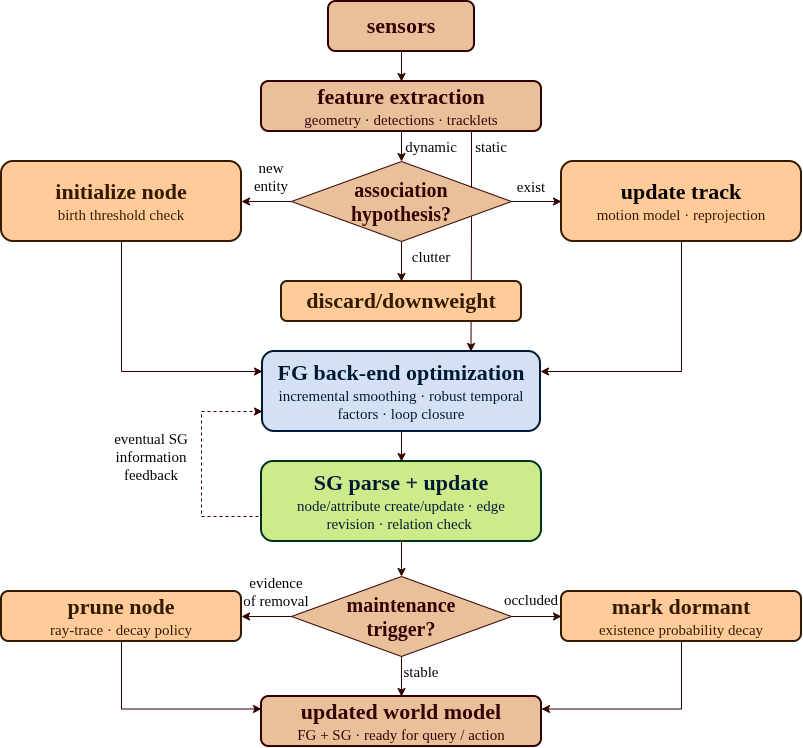
\includegraphics[width=\columnwidth]{Figures/figure_operational_pipeline.png}
    \caption{Per-frame operational pipeline of the hybrid world model.}
    \label{fig:FG_SG_world_model_construction_maintenance_workflow}
\end{figure}
%\input{Sections/modeling_dynamics}
%% How to use it
\section{Interaction: Querying, Reasoning, and Action}\label{sec:querying_reasoning_action}
% Query types: symbolic, geomtric, probabilistic.
% action coupling: planning over abstraction, hierarchical planning, task conditioned subgraphs.
% dynamic updates: re-perception loops, correcting wrong nodes/edges over time.
The shift from static environmental representations to \textit{actionable spatio-temporal perception} marks a fundamental transition where the world model is no longer a passive record of geometry but an active substrate for robot reasoning and decision-making \cite{rosinol_3d_2020} \cite{bavle_slam_2023}.
The convergence of factor graphs, providing metric-semantic consistency, and (3D) scene graphs, offering hierarchical relational logic, enables a rich set of interaction modalities, encompassing multi-modal querying, hierarchical planning, and closed-loop maintenance.

\subsection{Multi-Modal Query Paradigms}\label{sec:querying_reasoning_action_query}
The literature identifies three primary query modalities that leverage the structured nature of hybrid world models:
% It misses the link with the dynamic environment!

\noindent\textbf{Geometric-Metric Queries:} leveraging the low-level metric semantic mesh or factor-graph-backed pose and places layers, agents execute queries for fast collision checking via Bounding Volume Hierarchies\cite{rosinol_kimera_2021} and metric path planning\cite{catalano_3d_2025}, e.g. $A^*$ or Dijkstra.

\noindent\textbf{Symbolic-Semantic Queries:} hierarchical 3D Scene Graphs support high level symbolic commands, such as ``get the medication bottle from the nightstand''\cite{catalano_3d_2025}, often assisted by LLMs to achieve long-term trajectory prediction\cite{gorlo_long-term_2024}. 
By grounding abstract terms in specific room or object nodes, the model resolves spatial relationships, such as \textit{on}, \textit{inside}, to isolate target entities.
These language-grounded mechanisms operate primarily at the exploitation layer: they consume semantic and relational world-model state rather than replacing the geometric estimation machinery used to construct it. 
Their comparison with factor-graph approaches is therefore meaningful in terms of the downstream capabilities enabled by the representation, rather than through a common estimation or uncertainty model.
Open-vocabulary frameworks further extend this to previously unseen categories using CLIP-based embeddings. 

\noindent\textbf{Probabilistic-Expectation Queries:} %To address partial observability, systems like Belief Scene Graphs \cite{saucedo_estimating_2025} introduce \textit{blind nodes} representing expected but unobserved objects.
% These modules use Graph Convolutional Networks to predict likely object or agents locations on learned co-occurrence patterns and common sense, such as expecting a stove to be in a kitchen, or classrooms having similar and repeating desks patterns. 
systems like Belief Scene Graphs \cite{saucedo_estimating_2025} repurpose blind nodes (Section \ref{sec:dyn_world_model_representations_scene_graphs}) to answer ``what is likely present, even if unobserved'', using the same GCN-based co-occurrence priors to predict object or, potentially, agent locations.

While these three paradigms differ in representation and reasoning mechanism, Table~\ref{tab:query_paradigms} reveals a shared limitation: each is fundamentally a query over a \textit{static} world snapshot. 
Geometric-metric queries assume the underlying mesh remains valid until the next re-planning trigger; symbolic-semantic queries assume the scene graph reflects the current arrangement of entities, requiring re-detection or change-point tracking to remain accurate; and probabilistic-expectation queries model uncertainty over \textit{unobserved} space rather than uncertainty over \textit{time}, leaving moving or transient objects largely unaddressed. 
Bridging this gap, recent work on dynamic scene graphs and continual re-localization (e.g.,~\cite{ejaz2025situationallyawarepathplanningexploiting}) begins to treat the world model itself as a temporally evolving belief, suggesting that future query paradigms may need to fuse the spatial reasoning surveyed above with explicit temporal consistency mechanisms.

\begin{table*}[t]
\centering
\scriptsize
\setlength{\tabcolsep}{3pt}
\renewcommand{\arraystretch}{0.0}
\caption{Comparison of the three query paradigms over hybrid world models.}
\label{tab:query_paradigms}
\begin{tabularx}{\textwidth}{@{}l X X X@{}}
\toprule
\textbf{Dimension} & \textbf{Geometric-Metric} & \textbf{Symbolic-Semantic} & \textbf{Probabilistic-Expectation} \\
\midrule
Representation &
Metric-semantic mesh, factor-graph pose layers, occupancy/TSDF volumes &
Hierarchical 3D scene graph (room/object/relation nodes) &
Scene graph augmented with latent \textit{blind nodes} and learned priors \\
\addlinespace
Core question &
Is this space free? What is the shortest path from A to B? &
Where is object X? What satisfies relation $R$ to $Y$? &
What is \textit{likely} present, even if unobserved? \\
\addlinespace
Typical methods &
BVH collision checks~\cite{rosinol_kimera_2021}, $A^*$, Dijkstra, RRT*, ESDF planners &
Graph traversal/matching, LLM-grounded language-to-node resolution~\cite{gorlo_long-term_2024}, CLIP-based open-vocabulary retrieval &
GCNs, learned co-occurrence priors, Bayesian belief updates~\cite{saucedo_estimating_2025} \\
\addlinespace
% Example queries &
% ``Find a collision-free corridor wide enough for the robot base'' &
% ``Bring the red mug from inside the cabinet under the sink''&
% ``Estimate where the fire extinguisher is in this unexplored office''\\
% \addlinespace
Granularity &
Fine-grained, continuous/metric &
Discrete, categorical, relational &
Discrete, but probability-weighted over unobserved nodes \\
\addlinespace
Failure modes &
Degrades under sensor noise/incomplete reconstruction; costly at scale without hierarchical pruning &
Sensitive to grounding errors; brittle to novel categories without open-vocab support &
Priors can encode dataset bias; blind-node confidence is hard to calibrate \\
\addlinespace
Role of dynamics &
Assumes quasi-static mesh; requires re-planning triggers on change &
Assumes static graph; needs incremental updates from re-detection &
Models unobserved-space uncertainty, not temporal/moving-object uncertainty \\
\bottomrule
\end{tabularx}
\end{table*}

\subsection{Action Coupling and Hierarchical Planning}\label{sec:querying_reasoning_action_action}
Interaction with the environment is increasingly handled through abstractions that trade off model fidelity for computational efficiency \cite{ejaz2025situationallyawarepathplanningexploiting}.

\noindent\textbf{Hierarchical and Multi-Resolution Planning}: 3D Scene Graphs enable robots to decompose complex tasks across abstraction layers.
For instance, path planning can occur first at building or room level before refining to traversable place nodes, accelerating query times by several orders of magnitude compared to dense volumetric approaches \cite{viswanathan2024xflieleveragingactionablehierarchical} \cite{viswanathan2025spadescalablepathplanning} \cite{ejaz2025situationallyawarepathplanningexploiting} \cite{ray2024taskmotionplanninghierarchical}, and allowing for easier storage of pre-computed path when replanning is necessary \cite{ejaz2025situationallyawarepathplanningexploiting}.

\noindent\textbf{Task-Conditioned Subgraphs:} To manage the scale of massive environmental graphs, frameworks like \textit{SayPlan}\cite{rana2023sayplangroundinglargelanguage} and \textit{Clio}\cite{maggio_clio_2024} use ``task-driven'' abstraction. 
These systems interactively shrink the 3D Scene Graph by clustering and pruning nodes irrelevant to the current natural language mission, creating a minimal, actionable subgraph ready to use for the planner.

\noindent\textbf{Control-Centric Hierarchy:} Some architectures incorporate an \textit{Action Layer} directly into the scene graph \cite{ravichandran_hierarchical_2021}. 
This layer represents candidate robot actions, such as \textit{forward}, \textit{turn}, as graph nodes connected to semantic elements, grounding affordances, and next-step reasoning within the spatial model.

\subsection{Dynamic Updates and Closed-Loop Consistency}\label{sec:querying_reasoning_action_updates}
In non-stationary environments, maintaining the accuracy of the world model requires the continuous correction of nodes and edges as the scene evolves. 

\noindent\textbf{Re-Perception and Credibility Loops:} Systems like SG-Nav \cite{yin2024sgnav} implement a re-perception mechanism that evaluates the credibility of goal candidates. 
If a classification is found to be ambiguous or incorrect during closer inspection, the agent dynamically adjusts the graph structure in real time.

\noindent\textbf{Interaction-Aware Updates:} DovSG \cite{yan_dynamic_2025} and Lost\&Found\cite{behrens_lost_2025} detect hand-object contact events to update object poses and parent-child relations locally, without requiring a full-dense scene reconstruction. 

\noindent\textbf{Geometric Verification:} %To correct the graph over time, frameworks like Khronos \cite{schmid_khronos_2024} distinguish between \textit{absence of evidence}, i.e. occlusion, and \textit{evidence of absence}, i.e. actual removal. 
% By checking if sensor rays go through previously occupied volumes, the system can back-propagate removal events to prune old inactive nodes and maintain temporal consistency. 
Khronos \cite{schmid_khronos_2024} applies the removal-vs-occlusion check at the interaction layer, back-propagating confirmed removals to prune stale nodes and maintain temporal consistency.

\subsection{Functional Interaction and Action-Effect Reasoning}\label{sec:querying_reasoning_action_interaction}
Beyond spatial relations, recent world models explicitly encode \textit{functional} structure that captures how robot actions induce state changes in the environment.
Functional Scene Graphs model interactive elements such as handles, switches, and control surfaces as first-class nodes, and represent causal dependencies through directed functional relations (e.g. \textit{controls}, \textit{opens}, \textit{enables}) \cite{zhang_open-vocabulary_2025} \cite{rotondi_fungraph_2025}. 
This representation allows robots to reason about which actions are required to achieve a desired state change, effectively grounding manipulation and task planning directly in the world model.

Crucially, functional relations are activated through interaction: they are updated when actions are executed or when human–object interactions are observed. 
This enables localized, semantically meaningful graph updates without requiring global re-optimization or dense scene reconstruction, as demonstrated in interaction-aware systems such as DovSG \cite{yan_dynamic_2025} and Lost \& Found \cite{behrens_lost_2025}. 
By encoding action–effect couplings explicitly, functional scene graphs bridge symbolic task reasoning and geometric execution, providing a structured model for multi-step manipulation and interaction in dynamic environments.



% Emerging interaction paradigms extend beyond static relations to capture the operational and rhythmic logic of the world.

% \noindent\textbf{Functional Scene Graphs:} Frameworks like OpenFunGraph \cite{zhang_open-vocabulary_2025} explicitly model interactive elements, for instance handles, switches and knobs, and their directed functional edges, e.g. a switch \textit{controls} a light. 
% This enables robots to execute complex, multi-step tasks by reasoning about which elements trigger specific environmental functions.

% \noindent\textbf{4D Temporal Reasoning:} Systems like \textit{Aion} \cite{catalano_aion_2025} attach directional flow statistics (Maps of Dynamics) to navigational nodes. 
% By learning the rhythm, or seasonality, of human activity, the robot can proactively plan paths that avoid high-congestion areas or align with dominant traffic flows. 
% This is supported by "temporal ownership transfer", ensuring dynamics move with their associated nodes during pose graph loop closure. 


\section{Applications}\label{sec:applications}
% Dynamic SLAM: consistent world model under motion/change
% MOT + interaction understanding: Agents, intentions, trajectories
% Navigation and Planning: hierarchical routing, traversability graphs, task-level grounding
% Scene Understanding/Memory: retrivial, localization, long term mapping.
The dynamic world models presented throughout this paper are not limited in their generation, but their value is realized through the downstream tasks they can enable.
The shift from static, geometric maps to hybrid probabilistic graph representations that jointly handle geometry, semantics and temporal changes unlocks a richer set of robotic capabilities.
This section organizes these applications around four themes that progress from self-localization to high-level reasoning: robust SLAM and consistent world modeling under dynamics (Section \ref{sec:applications_slam_dynamics}), multi-object tracking and interaction understanding (Section \ref{sec:applications_mot}), navigation and hierarchical planning (Section \ref{sec:applications_navigation}), scene understanding, memory and long-term retrieval (Section \ref{sec:applications_scene_understanding}).
These downstream capabilities also inherit errors accumulated during perception, association, and scene-graph construction, following the propagation chain discussed in Section \ref{sec:uncertainty_types}.

\subsection{Robust SLAM and Consistent World Modeling under Dynamics}\label{sec:applications_slam_dynamics}
The most immediate application of dynamic world models is improving the robustness of self-localization and map building and updating when the environment contains moving or movable entities. 
In static-world SLAM, dynamic elements degrade trajectory estimation through incorrect data associations and inconsistent landmark observations, leading to the standard approach of outlier rejection but ending up discarding information that a richer model could exploit.
Tightly-coupled systems such as DynaSLAM II \cite{bescos_dynaslam_2021}, DynoSAM \cite{morris_dynosam_2025}, BodySLAM++\cite{henning_bodyslam_2023} and AirDOS \cite{qiu2022airdos} demonstrate that the joint-optimization formulation introduced in Section \ref{sec:dynamics_representations_agents} improves ego-trajectory accuracy compared to outlier-rejection baselines, since the cross-terms make self-localization and dynamic-entity tracking mutually reinforcing.
%demonstrate that jointly optimizing camera poses, static landmarks, and dynamic agents trajectories in a unified factor graph back-end improves ego-trajectory accuracy compared to outlier-rejection baselines, because the cross-terms introduced by spatiotemporal reprojection factors make self-localization and dynamic entity estimation mutually reinforcing. 
DynEMo-SLAM \cite{giberna_dynemo-slam_2025} applies this formulation in practice, allowing the SLAM back-end to benefit from semantic priors on entity motion while producing a richer joint world model.
%extends this to a hybrid factor-scene graph formulation including occasionally displaced objects, where dynamic entities are incorporated both as factor graph variables constrained by semantic motion models priors and as nodes in the scene graph, enabling the SLAM back-end to benefit from semantic priors on entity motion while simultaneously producing a richer world model.

The world model also needs to remain consistent across sessions and under long-term changes. 
% Khronos \cite{schmid_khronos_2024} addresses the spatio-temporal consistency problem by factorizing it into a fast active window for short-term agent dynamics and an asynchronous global process for long-term change detection, using ray-tracing evidence to distinguish between object removal and transient occlusion.
Khronos \cite{schmid_khronos_2024} applies the spatio-temporal mechanisms described in Section \ref{sec:dyn_world_model_representations_scene_graphs} and \ref{sec:construction_pipeline_graph_maintenance} at system scale, demonstrating that the same active-window/global-process split supports lifelong operation across extended deployments.
Systems like DPG-SLAM \cite{walcott-bryant_dynamic_2012} implement explicit forgetting policies, pruning nodes only when they no longer contribute topological information, thereby managing graph complexity without losing historical data.
These mechanisms are essential for robots operating across extended deployment horizons, such as warehouses, offices, and hospitals, where the entity population changes between sessions, and represent a direct application of the probabilistic birth-death modeling discussed in Section ~\ref{sec:construction_pipeline_graph_maintenance}.

\subsection{Multi-Object Tracking and Interaction Understanding}\label{sec:applications_mot}
Beyond robust self-localization, dynamic world models serve as the substrate for understanding the agents and objects that populate the environment. 
In tightly coupled SLAMMOT paradigm, the factor graph back-end estimates object trajectories jointly with the robot pose, providing smoothed, geometrically consistent tracks that  can exploit joint constraints between ego-motion and dynamic-entity motion, unlike standalone MOT formulations that estimate object tracks independently of the SLAM state. 
DynoSAM \cite{morris_dynosam_2025}, BodySLAM \cite{henning_bodyslam_2022} and AirDOS \cite{qiu2022airdos} generate 4D spatio-temporal maps of dynamic objects and agents as an output of their unified optimization, enabling downstream tasks such as trajectory prediction and collision forecasting.

For human agents specifically, BodySLAM \cite{henning_bodyslam_2022} and BodySLAM++ \cite{henning_bodyslam_2023} recover full SMPL body shape and pose jointly with camera trajectory (Section \ref{sec:dynamics_representations_agents}), producing a world model that captures postural state directly relevant to human-robot interaction and intention prediction. %go further by recovering full SMPL body shape and pose jointly with camera trajectory, producing world model that captures not only where a person is but also their postural state, information directly relevant to human-robot interaction and intention prediction.
The structured prior provided by the parametric body model acts as a strong regularizer that improves both the human pose estimate and the camera trajectory, particularly in scenes where humans occlude most of the field of view and purely geometric feature tracking fails. 
At the level of intentions and trajectories, Gorlo et al. \cite{gorlo_long-term_2024} use the temporal structure of a 3D dynamic scene graph, e.g. recognizing that a person moving toward a doorway is likely to exit, rather than relying solely on kinematic history.
Aion \cite{catalano_aion_2025} extends this predictive capability to activity forecasting, building a model of human rhythms that lets the robot anticipate congestion before it occurs. %further by learning directional flow statistics over navigational nodes, building a predictive model for human activity rhythms that enables the robot to anticipate congestion before it occurs. 

Scene graphs enrich this tracking with semantic understanding of interactions, like Lost \& Found \cite{behrens_lost_2025} and its human-object interactions triggering updates at graph edge level, effectively building a running causal system for tracking how the scene has changed due to human activity without requiring a full scene reconstruction after each interaction.

\subsection{Navigation and Hierarchical Planning}\label{sec:applications_navigation}
Dynamic world models directly inform navigation and planning by providing structured, multi-resolution representations that support both metric path execution and high-level task decomposition.
The hierarchical layers of 3D scene graphs allow planners to operate at an appropriate level of abstraction for the current task, consistently reducing computation compared to planning over dense volumetric maps \cite{ray2024taskmotionplanninghierarchical} \cite{viswanathan2025spadescalablepathplanning}. Ejaz et al. \cite{ejaz2025situationallyawarepathplanningexploiting} demonstrate this computation efficiency through situationally-aware path planning over 3D scene graphs, using the relational structure of the graph to select traversal sequences that account for both metric cost and semantic context. 

 In factor-graph-backed scene graphs, metric node positions can inherit the global consistency of the underlying geometric optimization, providing a geometrically grounded representation for downstream planning.  
SayPlan \cite{rana2023sayplangroundinglargelanguage} and Clio \cite{maggio_clio_2024} apply the task-driven pruning described in Section \ref{sec:querying_reasoning_action_action} to reduce planning complexity by orders of magnitude in large environments. %address scalability by using task-driven abstraction to prune the scene to a minimal actionable subgraph relevant to the current natural language mission, reducing planning complexity by orders of magnitude in large environments.

In dynamic environments, however, static planning assumptions break down: a path computed over the current scene graph may become infeasible as agents move, objects are displaced, or passageways are shut. 
The connection between the factor graph dynamics layer and the planning layer remains largely open. 
Current systems either replan from scratch on graph updates or maintain pre-computed paths that are invalidated when dynamic nodes change \cite{ejaz2025situationallyawarepathplanningexploiting}, a limitation that Aion's predictive flow statistics (Section \ref{sec:dyn_world_model_representations_scene_graphs}) begin to address by routing around congestion proactively\cite{catalano_aion_2025}.
The quality of the planning representation is therefore directly conditioned on the upstream estimation pipeline.
A localization or object-pose error primarily perturbs metric costs and collision geometry, whereas an incorrect association or relation can alter the topology presented to the planner, for example by assigning an obstacle to the wrong location or incorrectly representing a passageway as traversable.
These errors can consequently have different effects on navigation even when their representation-level accuracy metrics are similar.

\subsection{Scene Understanding, Memory, and Long-Term Retrieval}\label{sec:applications_scene_understanding}
The fourth identified application area treats the dynamic world model as a persistent, queryable memory that supports object retrieval, semantic localization and long-term scene understanding.
DovSG \cite{yan_dynamic_2025} demonstrates this for mobile manipulation, where the open-vocabulary 3D scene graph serves as the robot's persistent object memory, supporting natural language queries for object retrieval even after objects have been displaced by human interaction. % human interactions have displaced objects from their original locations, with local graph updates keeping the memory consistent without requiring full rescanning. 

% Belief Scene Graphs \cite{saucedo_estimating_2025} extend this memory to unobserved regions, using learned co-occurrence patterns to populate the scene graph with probabilistic blind nodes representing objects expected to exist based on commonsense spatial knowledge, e.g. a stove in a kitchen or a desk in a classroom. 
% This transforms the world model from a reactive record of observations into a predictive spatial memory that can guide active exploration and object search under partial observability.
Belief Scene Graphs \cite{saucedo_estimating_2025} extend this memory to unobserved regions, transforming the world model from reactive record into a predictive spatial memory that can guide active exploration under partial observability.
For manipulation, semantic and relational errors can be more consequential than small metric errors: a well-localized object with an incorrect class, state, relation may lead the robot to select the wrong target or execute an invalid interaction, whereas moderate pose error may still be corrected through local re-perception before execution.

\bigskip

Across all four application areas,  the surveyed systems illustrate how probabilistic geometric estimation and semantic-relational abstraction can provide complementary capabilities for estimation, prediction, planning and interaction. 
This architectural complementarity suggests that hybrid factor graph-scene graph representations are a promising design direction for applications requiring both geometric consistency and semantic reasoning, although the surveyed evidence does not establish their general superiority over alternative representations.

%and that the downstream applications they enable are qualitatively beyond what either paradigm alone can support in dynamic environments.

\section{Evaluation Protocols, Datasets and Metrics}\label{sec:evaluation_metrics}
Evaluation can be considered at two complementary levels. 
Representation-level metrics assess the accuracy, consistency and efficiency of the world model itself, whereas task-level metrics assess whether that representation improves downstream robot behavior.
The former are necessary diagnostics, but lower trajectory error or higher scene-graph accuracy does not necessarily imply improved navigation or manipulation performance.
We therefore use task-level metrics specifically for evaluations in which the constructed world model is consumed by a downstream robotic or reasoning task and performance is measured at the level of that task, rather than inferred from representation accuracy alone.

\begin{table*}[!htbp]
  \caption{Public Datasets and Benchmarks for Dynamic SLAM and Object Tracking}
  \label{tab:datasets_benchmarks}
  \centering
  \scriptsize
  \adjustbox{max width=\textwidth, max totalheight=0.98\textheight}{%
  \setlength{\tabcolsep}{3pt}
  \renewcommand{\arraystretch}{1.15}
  \begin{tabularx}{\textwidth}{@{}X X X X X X X@{}}
    \toprule
    \textbf{Dataset} & \textbf{Key Features} & \textbf{Environment} & \textbf{Dynamics} & \textbf{Use Case} & \textbf{Sensors} & \textbf{Used In} \\
    \midrule
    \midrule
    \multicolumn{7}{@{}c}{\textbf{I. Public Outdoor and Urban Driving Benchmarks}} \\
    \midrule
    KITTI Tracking/Odometry \cite{gaidon2016virtual} & Grayscale and RGB stereo, GPS, IMU, 3D LiDAR & Urban/Highway & Vehicles, pedestrians & High-speed dynamics, ego-motion ambiguity & GPS, IMU, 3D LiDAR,  RGB & \cite{bescos_dynaslam_2021}, \cite{brink_using_2016}, \cite{morris_importance_2024}, \cite{tian_dl-slot_2024}, \cite{tian_dynaquadric_2024} \\
    nuScenes \cite{caesar_nuscenes_2019} & 3D MOT (AMOTA), urban LiDAR detections & Urban & High traffic density & Multi-object tracking, accuracy evaluation & LiDAR,  RGB & \cite{zaech_learnable_2022} \\
    Virtual KITTI \cite{geiger_vision_2013} & Synthetic, photo-realistic, ground truth camera/object poses & Urban/Highway & Vehicles, pedestrians & Depth error isolation, object segmentation &  RGB,  & \cite{henein_dynamic_2020} \\
    Victoria Park \cite{guivant_simultaneous_2002} & 2D odometry, landmark observations (trees), simulated northward movement & Urban & Corrupted landmarks & Solver divergence, robustness testing & Laser scan, GPS & \cite{lingzhu_xiang_robust_2015} \\
    Alcazar of Seville \cite{iros14-frog} & Visual-stereo, dynamic pedestrians & Indoor/Outdoor & Pedestrian dynamics & Re-localization, landmark stability & Stereo RGB, Laser scanners & \cite{lingzhu_xiang_robust_2015} \\
    \midrule
    \midrule
    \multicolumn{7}{@{}c}{\textbf{II. Public Indoor and Semantic Mapping Datasets}} \\
    \midrule
    OpenLORIS-Scene \cite{shi_are_2019} & Office and supermarket environments, lifelong SLAM & Indoor & Pedestrian occlusion, scene changes & Long-term SLAM, furniture relocation & RGB-D, Semantic Labels & \cite{wang_semantic_2023}, \cite{ding_dynamic_2025} \\
    ScanNet \cite{dai_scannet_2017} & 1500+ RGB-D sequences, indoor spaces & Indoor & Static and dynamic objects & 3D scene graph construction, object relationships \& reconstruction & RGB-D, Semantic Labels & \cite{kim_3-d_2020} \\
    Matterport3D \cite{chang_matterport3d_2017} & 35 semantic classes, residential/commercial spaces & Indoor & Room layouts, objects & Learning co-occurrence, spatial distribution & RGB-D, 3D Models & \cite{saucedo_estimating_2025} \\
    TUM RGB-D \cite{sturm_benchmark_2012} & Office sequences, Kinect sensors, Vicon motion capture & Indoor & Walking, desk movements & High/Low dynamics, object tracking & RGB-D, Motion Capture & \cite{wang_semantic_2023} \\
    Bonn RGB-D Dynamic\cite{palazzolo2019iros} & Moving people interacting with moving objects & Indoor & Humans, Objects & Multi-object tracking Scene reconstruction & RGB-D  & \cite{cheng2022sg}\\
    Oxford Multimotion Dataset (OMD) \cite{judd_oxford_2019} & Swinging cubes, unconstrained motion & Indoor & Non-planar, fast-moving objects & Challenging dynamic tracking & Stereo, RGB-D, IMU, Vicon motion capture & \cite{gou_visual_2024}, \cite{morris_importance_2024}, \cite{morris_dynosam_2025} \\
    InCrowd-VI \cite{bamdad2024incrowd} & Indoor crowded environments & Indoor & Walking, crowded scenes & Indoor pedestrian-rich human navigation & RGB, IMU & \cite{bamdad2024incrowd} \\
    \midrule
    \midrule
    \multicolumn{7}{@{}c}{\textbf{III. Synthetic and Semi-Synthetic Environment Simulators}} \\
    \midrule
    TESSE Simulator \cite{ravichandran_bridging_2020} & Short-term dynamics, long-term changes, precise ground truth & Indoor & Walking, bouncing balls, furniture changes & Controlled ablation studies & RGB, Depth & \cite{schmid_khronos_2024} \\
    VirtualHome \cite{puig_virtualhome_2018} & Object movements in household routines, 50+ days & Indoor & Object movement in routine activities & Object tracking, daily activities & RGB & \cite{patel_proactive_2022} \\
    CARLA Simulator \cite{dosovitskiy_carla_2017} & Urban scene graph partitioning, weather dynamics & Urban & Traffic, pedestrian dynamics & Scene graph partitioning, dynamic environments &  RGB, LiDAR & \cite{greve_collaborative_2024} \\
    Dynamic House Simulator  \cite{kurenkov_modeling_2023} & Household dynamic objects, movement between furniture & Indoor & Object movement, probabilistic dynamics & Link prediction, dynamic environments & RGB & \cite{kurenkov_modeling_2023} \\
    \midrule
    \midrule
    \multicolumn{7}{@{}c}{\textbf{IV. Specialized Benchmarks and Self-Collected Data}} \\
    \midrule
    VIODE \cite{minodaRAL2021} & UAV-based visual-inertial odometry, extreme motions, occlusion, Ground truth poses & Outdoor & UAV in parking lot, dynamic agents & Real-time update, occlusion handling & Stereo RGB, IMU  & \cite{morris_dynosam_2025} \\
    TartanAir Shibuya \cite{tartanair2020iros}  & 30+ humans, dense urban crossing & Urban & Non-rigid, crowded scenes, Ground truth poses & Robustness in crowded environments & Stereo RGB, Depth  & \cite{morris_dynosam_2025} \cite{qiu2022airdos} \\
    uHumans/uHumans2 \cite{rosinol_kimera_2021} & Unity-based simulator, 12-60 human agents, SMPL meshes, Ground truth poses & Indoor/Outdoor & Dense human tracking & Human interaction, dynamic tracking & Stereo RGB, Depth, IMU  & \cite{rosinol_kimera_2021} \\
    FunGraph3D \cite{zhang_open-vocabulary_2025} & iPad Pro video, high-fidelity laser scans, Apple Vision Pro, Functional annotations & Indoor/Outdoor & Functional relationships (e.g., switches) & Functional annotation, relationship tracking & RGB-D/LiDAR, Laser Scan, egocentric video & \cite{zhang_open-vocabulary_2025} \\
    OC-NaVQA \cite{gorlo_describe_2025} & Object-centric NaVQA, spatio-temporal Q\&A, Ground truth Q\&A labels & Indoor/Outdoor & Static and dynamic environments & Question answering, memory sequences & Stereo RGB, RGB-D, LiDAR, IMU & \cite{gorlo_describe_2025} \\
    Husky/Spot Field Tests & Real university halls/offices, LiDAR and RGB-D sensors & Indoor & Dynamic agents (robots, pedestrians), dynamic objects & Real-time performance validation & LiDAR, RGB-D & \cite{schmid_khronos_2024}, \cite{giberna_dynemo-slam_2025} \\
    \bottomrule
  \end{tabularx}
  }
\end{table*}

\begin{table*}[!htbp]
\caption{Metric catalog for representation-level and task-level evaluation of dynamic SLAM (FG) and scene graph (SG) systems .}
\label{tab:metrics_table}
\centering
\scriptsize
\setlength{\tabcolsep}{3pt}
\renewcommand{\arraystretch}{1.15}
\begin{tabularx}{\textwidth}{@{}X l X@{} r}
\toprule

\textbf{Metric} & \textbf{Type} & \textbf{What it measures / notes} & \textbf{Used in} \\

\midrule

\textbf{ATE (RMSE/median)} & Trajectory & 
Absolute trajectory error vs ground truth; report RMSE + median, and whether aligned (SE(3)/Sim(3)). 
& \cite{bescos_dynaslam_2021} \cite{morris_dynosam_2025} \cite{giberna_dynemo-slam_2025}\\
\textbf{RPE ($\Delta t$ / $\Delta s$)} & Trajectory & Relative pose error; clarifies short-term drift; specify interval. 
& \cite{bescos_dynaslam_2021} \cite{morris_dynosam_2025} \cite{morris_importance_2024}\\
\textbf{Drift (m/100m, deg/100m)} & Trajectory & 
Aggregate drift over distance; common in automotive datasets. 
& \cite{rosinol_kimera_2021}\\
\textbf{Relocalization success rate} & Trajectory & 
Fraction of trials where tracking is recovered after dropout/occlusion. 
& \cite{vega_torres_bim-slam_2023} \cite{wang_semantic_2023}\\
\textbf{CS-R (Correctness Score of Re-Localization)} & Trajectory &
Reliability of re-localization events in dynamic scenes; typically validates that a declared relocalization is correct (not a false positive). 
& \cite{wang_semantic_2023}\\
\textbf{Failure rate / time-to-failure} & System & 
Robustness under dynamics; define failure criterion (e.g. lost tracking $>$ N frames). 
& \cite{scherer_ogm2pgbm_2023}\\

\midrule

\textbf{Runtime (Hz/FPS), latency (ms)} & System & 
Throughput and per-module latency; note hardware and whether real-time. 
& \cite{behrens_lost_2025} \cite{bescos_dynaslam_2021} \cite{schmid_khronos_2024}\\
\textbf{CPU/GPU, memory footprint} & System & 
Resource profile for deployability comparisons. 
& \cite{ferraina_lost-3dsg_2026}\\

\midrule

Geometric RMSE / surface distance & Map & 
Geometric discrepancy between reconstructed surface/point cloud and a reference model, specifying registration procedure. . 
& \cite{rosinol_kimera_2021} \cite{yan_dynamic_2025}\\
\textbf{Map IoU} & Map & Overlap between predicted and GT occupancy grids; specify resolution and thresholding. 
& \cite{rosinol_kimera_2021}\\
\textbf{TP rate (2D / BEV / 3D)} & Map &
True positive rate for occupancy estimation across viewpoints/representations; report the corresponding FP/FN definitions. 
& \cite{zhang_semantic-integrated_2026} \cite{bescos_dynaslam_2021}\\
\textbf{SCDA (Scene Change Detection Accuracy)} & Change &
Accuracy of detecting voxel-level or object-level changes over time; clarify temporal window and whether class-conditioned. 
& \cite{yan_dynamic_2025}\\

\midrule

\textbf{Mask IoU / mIoU} & Semantics & 
Segmentation quality for dynamic masking or semantic labels. 
& \cite{rosinol_kimera_2021}\\
\textbf{Precision/Recall/F1 (objects)} & Semantics & 
Detection/instance metrics; specify IoU threshold (e.g. 0.5). 
& \cite{schmid_khronos_2024}\\
\textbf{Motion Error (ME)} & Motion &
Frame-agnostic object motion error evaluated in the ground-truth object frame; helps compare methods using different reference frame conventions. 
& \cite{morris_dynosam_2025} \cite{morris_online_2025}\\

\midrule

\textbf{MOTA / AMOTA / MOTP} & Tracking &
Classic multi-object tracking metrics (association + localization); sensitive to thresholds and missed detections. 
& \makecell{\cite{gou_visual_2024} \cite{tian_dl-slot_2024} \cite{zaech_learnable_2022} \\ \cite{zhang_semantic-integrated_2026} \cite{gou_visual_2024} \cite{bescos_dynaslam_2021}} \\
\textbf{ID Switches} & Tracking &
Counts identity swaps in tracking; lower is better. 
& \cite{zhang_semantic-integrated_2026} \cite{zaech_learnable_2022}\\
\textbf{Fragments (track fragmentation)} & Tracking &
Counts interruptions/splits in a trajectory; measures continuity of tracks. 
& \cite{zhang_semantic-integrated_2026}\\
\textbf{IDF1} & Tracking &
Identity-based F1; balances correct associations over time. 
& \cite{zhang_semantic-integrated_2026}\\
% \textbf{HOTA} & Tracking &
% Higher-order tracking accuracy (joint detection + association quality). 
% & \\

\midrule

\textbf{Node Precision/Recall/F1} & Graph &
Correctness of entity discovery (rooms/walls/objects) in scene graphs; depends on matching policy between predicted and GT nodes. 
& \cite{zhang_open-vocabulary_2025} \cite{ferraina_lost-3dsg_2026}\\
\textbf{Edge Precision/Recall/F1 / edge prediction/accuracy} & Graph &
Correctness of predicted relations (adjacent-to, in-room, supports, etc.); report relation set and matching rules. 
& \cite{zhang_open-vocabulary_2025}\\
\textbf{Spurious \& Missing Entities} & Graph &
Human-judgment metric counting incorrect (spurious) or omitted (missing) nodes/edges in constructed SGs. 
& \cite{kim_3-d_2020}\\
\textbf{Precision/Recall of scene parsing} & Parsing &
Accuracy of partitioning places into rooms or higher-level structures (often computed from segmentation or region adjacency). 
& \cite{rosinol_3d_2020}\cite{rosinol_kimera_2020}\\
\textbf{Graph Edit Distance (GED)} & Graph &
Structural similarity to GT graph; sensitive to node/edge labels,  matching and edit-cost definition. 
& \textcolor{yellow}{\cite{milewski2026human}}\\
\textbf{Temporal  graph change} & Graph-time &
 Change in graph structure over time (e.g., additions/deletions per minute, or lifetime distributions); normalization is required when graph size differs. 
& \cite{guo2026ssprcd} \\

\midrule

\textbf{NDCG (Normalized Discounted Cumulative Gain)} & Ranking &
Quality of predicted rankings (e.g., likelihood-ranked object locations); requires relevance labels and a cutoff $K$. 
& \cite{kurenkov_modeling_2023}\\

\midrule

\textbf{NEES / $\chi^2$ consistency} & Prob. (FG) &
Consistency of estimated state uncertainty against ground-truth error; important when works claim probabilistic reliability.
&\cite{ila2009information}\\

\midrule
%\multicolumn{3}{@{}l}{\textbf{Semantic reasoning and downstream task metrics}}\\
\midrule

\textbf{Descriptive question accuracy (SQA)} & Reasoning &
Accuracy on spatio-temporal question answering using 4D/temporal scene graphs. 
& \cite{gorlo_describe_2025}\\
\textbf{ADE (Avg. Displacement Error)} & Prediction &
Average distance between predicted and GT trajectories (e.g., human motion). 
& \cite{gorlo_long-term_2024}\\
\textbf{BoN ADE (Best-of-N ADE)} & Prediction &
Minimum ADE over $N$ sampled predictions; measures multi-modal forecasting quality. 
& \cite{gorlo_long-term_2024}\\
\textbf{Task success rate} & Task &
Completion rate of robot tasks informed by the world model (e.g., pick-and-place); specify task definition and failure modes. 
& \cite{yan_dynamic_2025}\\
\textbf{BLEU / METEOR / BERTScore} & Language &
Similarity of generated textual SG annotations to references; report whether multiple references are used and tokenization details. 
& \cite{linok_dygenc_2025}\\

\bottomrule
\end{tabularx}
\end{table*}


\subsection{Protocols}\label{sec:evaluation_metrics_protocols}
%Protocols: per-sequence evaluation; multi-run statistics; dynamic severity sweeps; relocalization dropouts; multi-session/long-term changes; ablations (robust loss, dynamic filtering, SG update policy).
A thorough analysis of the evaluation protocols reveals a rigorous methodological framework designed to validate the robustness of world models against non-stationary environments.
These protocols go beyond traditional SLAM metrics, including stochastic analysis, longitudinal studies and modular ablations to isolate the effect of various architectural components. 
Moreover, research in dynamic SLAM has shifted towards validating the efficacy of the system in and for specific use cases.
Across the surveyed literature, evaluation protocols combine conventional SLAM metrics with robustness tests, longitudinal evaluation, and targeted ablations, although the exact protocol varies considerably across systems and applications. Application-specific evaluations are also increasingly used to assess the benefits of dynamic world models for particular downstream tasks.


\subsubsection{Per-Sequence and Multi-Run Evaluation}
Evaluation is commonly reported per sequence, while several surveyed works additionally repeat runs to quantify stochastic or implementation-dependent variability :

\begin{itemize}
    \item \textbf{Per-Sequence Analysis}:  Many surveyed works report results separately for each sequence to expose variations in environmental conditions, dynamic density and feature availability \cite{tian_dl-slot_2024} \cite{giberna_dynemo-slam_2025} \cite{zhang_semantic-integrated_2026}.
    \item \textbf{Stochasticity Management}: To mitigate the impact of random initialization in particle filters or the non-deterministic nature of multi-threaded optimization, experiments are executed multiple times.
     Reported practices include running each sequence multiple times and reporting the median value \cite{zhang_semantic-integrated_2026} or average \cite{scherer_ogm2pgbm_2023}.
    Other collaborative frameworks report mean and standard deviation over several randomly initialized runs to quantify stability \cite{greve_collaborative_2024}.
\end{itemize}

\subsubsection{Dynamic Severity Sweeps}
Evaluation protocols frequently involve sweeping through levels of environmental complexity to test the limits of dynamic robustness.

\begin{itemize}
    \item \textbf{Entity Density Scalability}: The uHumans and uHumans2 datasets are used to evaluate how spatial perception engines handle environments with increasing numbers of dynamic entities, ranging from 12 to 60 human agents \cite{rosinol_3d_2020}. Similar approaches are partaken when the dynamics in the scene are displaced objects rather than continuously moving humans \cite{ferraina_lost-3dsg_2026}. Also self-collected datasets are generated accounting for different progressive levels, densities and complexities of dynamic entities populating the scene \cite{giberna_dynemo-slam_2025}.
    \item \textbf{Dynamic Entity Types}: Taking into account that different kinds of dynamics can occur in the scene, e.g. persistently moving agents and occasionally displaced objects, the systems' generalization capabilities are often evaluated by testing  subsets or different configurations of possible dynamics occurring in the scene \cite{giberna_dynemo-slam_2025}.
    \item \textbf{Clutter and Deviation Levels}: In BIM-based localization, scenarios are designed to progressively increase the level of clutter, thereby decreasing the overlap with permanent building objects \cite{vega_torres_bim-slam_2023} \cite{shaheer_tightly_2025}.
    \item \textbf{Controlled Configuration Sweeps}: Navigation models are tested against varying obstacle configurations to ensure that learned policies generalize across different collision trajectories \cite{maguire_lidar-only_2025}. 
\end{itemize}

\subsubsection{Relocalization Dropouts and Success Rate}
The robustness of the world model is tested through its ability to recover from tracking loss, particularly when dynamic occlusion causes feature dropouts. 

\begin{itemize}
    \item \textbf{Sequential Retrieval Tests}: Systems are evaluated by sequentially feeding data from different sessions and counting the number of successful against unsuccessful relocalization events \cite{wang_semantic_2023}.
    \item \textbf{Convergence Metrics}: Success is often defined by a threshold-based protocol, where a method is deemed to have converged if the pose estimate, either of the exploring robot's trajectories or detected entities, stabilizes within a specific distance of the ground truth within a set percentage of the sequence length\cite{vega_torres_bim-slam_2023} \cite{morris_importance_2024}.
    \item \textbf{Initialization and Hand-off}: Some protocols evaluate the efficiency of switching from a stochastic global localizer to a precise graph-based localization algorithm once a covariance threshold is met \cite{scherer_ogm2pgbm_2023}.
\end{itemize}

\subsubsection{Multi-Session and Long-Term Change Protocols}
Lifelong autonomy is validated through longitudinal data collection and multi-pass traversal.

\begin{itemize}
    \item \textbf{Long-Term Monitoring}: Systems are evaluated on their ability to update object probabilities across extensive periods \cite{gomez_object-based_2020} \cite{patel_proactive_2022}.
    \item \textbf{Incremental Pass Validation}: Protocols include repeated traversals of the same environment to determine if the model can successfully ``forget'' ephemeral data and identify static  structural components \cite{walcott-bryant_dynamic_2012}.
    \item \textbf{Consecutive Task Execution}: Robots are tested on their ability to complete consecutive manipulation tasks without manual resets, ensuring the updated 3D scene graph remains actionable after manual modification of the environment \cite{yan_dynamic_2025}.
\end{itemize}

\subsubsection{Systematic Ablation Studies}
Ablation protocols are essential for isolating the contribution of proposed factors, modules and policies.

\begin{itemize}
    \item \textbf{Dynamic Filtering Modules}: Protocols isolate the dynamic entities or features removal module to identify the best trade-off for loop closure quality \cite{giberna_dynemo-slam_2025}.
    \item \textbf{Scene Graph Update Policies}: Researchers ablate the logic used for graph maintenance, such as the effectiveness of \textit{sequential reasoning} in functional graphs \cite{zhang_open-vocabulary_2025} or the utility of \textit{region clustering} and \textit{frame selection heuristics} \cite{gorlo_describe_2025} or \textit{keyframe selection policies} \cite{giberna_dynemo-slam_2025} in 4D scene graph generation.
    \item \textbf{Factor-Level Ablations}: In tightly-coupled systems, models are evaluated with and without specific constraints, such as \textit{non-rigid factors} for humans or \textit{rigid factors} for objects, to verify their individual contributions to trajectory accuracy and world model generation \cite{giberna_dynemo-slam_2025} \cite{ding_dynamic_2025}.
\end{itemize}


Viewed through the representation-versus-utility distinction introduced above, most surveyed protocols primarily evaluate representation-level robustness: they perturb dynamic density, tracking conditions, map structure, or individual system components and measure the resulting estimation or reconstruction quality.
Task-level evaluation is less common.
For example, consecutive task-execution protocols directly test whether an updated scene graph remains useful for manipulation \cite{yan_dynamic_2025}, whereas many dynamic SLAM evaluations terminate at trajectory, tracking or map-quality metrics.
Consequently, the literature provides more evidence about whether a world model is geometrically or structurally accurate than about how much that accuracy improves downstream robotic behavior. 


\subsection{Datasets}\label{sec:evaluation_metrics_datasets}
%Datasets: split by sensing (RGB-D / stereo / LiDAR / multi-modal), and by dynamics type (moving objects, crowds, structural changes, illumination/weather changes, multi-session).
The evaluation of hybrid world models, integrating scene graphs and/or factor graphs, and spatio-temporal dynamics, relies on a hierarchical selection of commonly employed datasets ranging from established autonomous driving benchmarks to specialized indoor semantic simulators.
Additionally, to assess the system behavior on specific situations, self-collected datasets presenting peculiar kinds of environments and dynamics are created, either in real world or simulation. 
These datasets can be categorized by their environmental focus, sensor suites, and the specific nature of the dynamics they encapsulate. 
Table \ref{tab:datasets_benchmarks} reports the most commonly used publicly available datasets, benchmarks and simulators. 

\subsection{Metrics}\label{sec:evaluation_metrics_metrics}
%Metrics: group into trajectory, map geometry, semantics/tracking, graph structure, system/runtime, and probabilistic consistency.
The metrics in Table \ref{tab:metrics_table} fall into two broad classes.
Representation-level metrics evaluate trajectory estimation, map geometry, perception and tracking, graph structure, computational performance, and probabilistic consistency.
Task-level metrics instead evaluate the utility of the resulting world model for reasoning and action, such as question answering or task success.
Improvements in representation-level metrics do not necessarily translate into higher task-level utility, motivating the evaluation gap discussed in Section \hyperref[sec:open_challenges_metrics_gap]{X-C(d)}.
The distribution of metrics in Table \ref{tab:metrics_table} also reveals an evaluation imbalance in the current literature.
Trajectory, mapping, tracking and graph-structure accuracy have well-established quantitative measures, whereas end-to-end task utility is evaluated less systematically and with application-specific criteria.
Moreover, the surveyed works rarely measure both levels under the same controlled perturbation, so the relationship between an improvement in representation quality and the corresponding improvement in task performance is generally unknown. 
This prevents, for example, determining how a reduction in object-pose or an improvement in relation accuracy translates into navigation or manipulation success.


\section{Comparative Analysis of Representative Systems}\label{sec:taxonomy}
The literature on world modeling in dynamic environments spans a wide range of representational choices, inference strategies and application targets.
While individual systems are often described in isolation, a comparative perspective is necessary to understand how these design decisions relate to one another and how different combinations of graphical models, dynamic handling, and uncertainty profiles emerge in practice. 
This section provides a structured comparison of the surveyed \emph{systems} themselves, classifying graph-based dynamic world models for robotics along a set of common axes.
Rather than ranking methods by performance, the comparison aims to map the design space, highlighting recurring architectural patterns and characteristic trade-offs across factor-graph-based, scene-graph-based and hybrid representations.

\subsection{Axes of Comparison}\label{sec:taxonomy_axes}
The analysis organizes existing approaches along several dimensions that recur throughout the surveyed literature:
\begin{itemize}
    \item \textbf{Graph Stack}: the primary representational backbone employed by the system, distinguishing between factor graphs (FG), scene graph (SG), and hybrid architectures that explicitly maintain both representations with cross-representation correspondence, as defined in Section \ref{sec:background_hybrid};
    \item \textbf{Dynamics Type}: the class of environmental change modeled, using the same three-tier Temporal Horizon distinction introduced in Section \ref{sec:taxonomy_dynamics} (short-term dynamics, semi-static changes, and long-term structural evolution);
    \item \textbf{Represented Scene}: the operational context, such as indoor, outdoor, or any environment;
    \item \textbf{Data Association Strategy}: the mechanism used to link observations over time, ranging from deterministic matching to probabilistic multi-hypothesis methods or learned similarity models;
    \item \textbf{Inference Policy}: the underlying inference method, including batch maximum a posteriori (MAP) optimization, incremental smoothing, filtering-based approaches, or variational inference;
    \item \textbf{Uncertainty Profile}:  which uncertainty classes are represented (\textit{geometric state, \textit{semantics}, \textit{data association}, \textit{existence}, and \textit{relations}), and whether their treatment is explicitly probabilistic, heuristic or deterministic};
    \item \textbf{Sensor}: the employed sensing inputs used to build the world model;
    \item \textbf{System Properties}: 
    \begin{itemize}
        \item \textbf{RT} denotes reported real-time operation under the hardware, sensing configuration, scene complexity, and experimental conditions of the original work. It is therefore not a normalized cross-method performance comparison. \checkmark~ indicates that end-to-end online operation was experimentally demonstrated at the operating rate reported by the authors; $\sim$ indicates partial/module-level real-time operation or architectural support without end-to-end demonstration; \xmark~ indicates that real-time was not demonstrated or reported.
        \item \textbf{OV}: \checkmark~ requires experimental operation beyond a fixed predefined semantic vocabulary; $\sim$ denotes use of open-vocabulary components without end-to-end evaluation; \xmark~ denotes no reported demonstration.
        \item \textbf{MR}: \checkmark~ requires an experimental demonstration in which multiple robots collaboratively construct, update, or use a shared representation; $\sim$ denotes architectural or component-level multi-robot support without end-to-end demonstration; \xmark~ denotes no reported demonstration.
    \end{itemize}
    \item \textbf{Downstream Usage}: the primary tasks specifically enabled or targeted by the representation, such as robust SLAM, navigation, manipulation, interaction understanding, or prediction. This axis identifies the intended use of the representation and should not by itself be considered as evidence of improved task-level performance; such evidence requires an explicit task-level evaluation as defined in Section \ref{sec:evaluation_metrics}. 
\end{itemize}
These axes stem from the three research questions posed in Section \ref{sec:introduction}: Graph Stack, Dynamics Type, and Represented Scene characterize \emph{what is represented} (RQ1); Data Association Strategy, Inference Policy, Uncertainty Profile, and Sensor  characterize \emph{how the representation is constructed and maintained} (RQ2); and System Properties, and Downstream Usage characterize \emph{how the representation is exploited} (RQ3). 
Together, these axes provide a unified lens through which heterogeneous systems can be compared across all three questions simultaneously, without assuming a notion of optimality.

\subsection{Comparison of Existing Approaches}\label{sec:taxonomy_taxonomy}
Table \ref{tab:taxonomy_overview} summarizes representative works in the literature according to the comparison dimensions defined above.
The listed systems are grouped by their underlying graph stack, enabling a direct comparison between factor-graph-based methods, scene-graph-centric approaches, and hybrid representations that integrate probabilistic estimation with semantic abstraction.
Because the surveyed systems are evaluated using different sensors, datasets, tasks, and metrics, this comparison supports an architectural analysis rather than a performance ranking. 
The comparison axes should not be interpreted as implying a common objective across all representational paradigms.
Dimensions such as sensing, dynamics coverage, data-association strategy, system properties and downstream usage can be compared descriptively across architectures, whereas inference policy and uncertainty profile characterize paradigm-specific mechanisms rather than values on a common performance scale. 
For example, learned semantic confidence scores, language-model outputs, and covariance-based probabilistic estimates represent fundamentally different quantities and should not be treated as equivalent uncertainty measures.
Accordingly, the reported system-property indicators summarize the level of evidence provided by the original works under their evaluated configurations, rather than intrinsic system capabilities, and differences in reported downstream performance cannot generally be attributed to the representation choice alone.
Moreover, the surveyed literature does not provide a standardized metric or controlled benchmark that isolates the effect of the representation architecture itself.
Existing metrics quantify individual aspects, such as geometric accuracy or downstream task success, but do not define a common measure of superiority across FG, SG, and hybrid FG-SG architectures.

\begin{table*}[htbp]
\caption{Comparative analysis of representative
probabilistic graph-based \emph{systems} for robotics in dynamic
environments.}
  \label{tab:taxonomy_overview}
  \centering

  \adjustbox{max width=\textwidth, max totalheight=0.85\textheight}{%
  \scriptsize
  \setlength{\tabcolsep}{2pt}
  \renewcommand{\arraystretch}{0.2}
  \setlength{\extrarowheight}{-2pt}
  \setlength{\aboverulesep}{0.2ex}

    \begin{tabularx}{\textwidth}{@{}
      >{\raggedright\arraybackslash}l  % Work
      >{\centering\arraybackslash}p{1.0cm}   % Graph stack 
      >{\raggedright\arraybackslash}X        % Nodes
      >{\raggedright\arraybackslash}X        % Edges
      >{\raggedright\arraybackslash}X        % Dynamics type
      >{\raggedright\arraybackslash}X        % Represented scene
      >{\raggedright\arraybackslash}X        % Association
      >{\raggedright\arraybackslash}X        % Inference
      >{\raggedright\arraybackslash}X        % Uncertainty
      >{\raggedright\arraybackslash}X        % Sensors
      c c c                                  % RT OV MR
      >{\raggedright\arraybackslash}X@{}     % Downstream use
    }
    \toprule
    & \multicolumn{5}{c}{\textbf{Representation}} &
    \multicolumn{4}{c}{\textbf{Construction \& Maintenance}} &
    \multicolumn{4}{c}{\textbf{Exploitation}} \\
    \cmidrule(lr){2-6} \cmidrule(lr){7-10} \cmidrule(lr){11-14}
    \textbf{Work} & \textbf{Graph stack} & \textbf{Nodes} & \textbf{Edges} & \textbf{Dynamics type} &
    \textbf{Represented scene} &
    \textbf{Association} & \textbf{Inference} & \textbf{Uncertainty Profile} & \textbf{Sensors} &
    \textbf{RT} & \textbf{OV} & \textbf{MR} & \textbf{Downstream use} \\
    \midrule

    % ── FACTOR GRAPH ONLY ──────────────────────────────────────────────────────
    \multicolumn{14}{@{}c}{\textit{Factor graph (FG) only}} \\
    \midrule

    \makecell[l]{DynaSLAM II\\Bescos et al.\\ (2021)\cite{bescos_dynaslam_2021}} &
    \makecell[c]{FG} &
    \makecell[l]{Camera pose,\\object pose, \\velocity,\\points} &
    \makecell[l]{reprojection \\error,\\motion error} &
    \makecell[l]{short-term \cmark\\semi-static \xmark\\long-term \xmark} &
    Outdoor &
    \makecell[l]{deterministic\\(ORB + IoU)} &
    \makecell[l]{batch\\MAP} &
    \makecell[l]{G:P, S:D,\\ A:D, E:D,\\ R:--} &
    \makecell[l]{Stereo or\\RGB-D} &
    \cmark & \xmark & \xmark &
    \makecell[l]{Collision \\avoidance\\+ SLAMMOT} \\
    \midrule

    \makecell[l]{Brink\\(2016)\cite{brink_using_2016}} &
    \makecell[c]{FG} &
    \makecell[l]{Image features,\\velocity} &
    \makecell[l]{same-object\\probabilistic\\ dependency} &
    \makecell[l]{short-term \cmark\\semi-static  \xmark\\long-term \xmark} &
    Any &
    \makecell[l]{deterministic\\(Delaunay\\ triangulation)} &
    \makecell[l]{incremental\\loopy BP} &
    \makecell[l]{G:P, S:--,\\ A:D, E:--,\\ R:--} &
    \makecell[l]{Stereo} &
    \xmark & \xmark & \xmark &
    \makecell[l]{Dynamic\\ object\\detection} \\
    \midrule

    \makecell[l]{DynoSAM\\Morris et al.\\(2025)\cite{morris_dynosam_2025}} &
    \makecell[c]{FG} &
    \makecell[l]{Camera poses,\\object \\motions/poses,\\map points} &
    \makecell[l]{point meas.,\\ odometry,\\object motion,\\ obj. smoothing,\\prior factors} &
    \makecell[l]{short-term \cmark\\semi-static \xmark\\long-term \xmark} &
    Any &
    \makecell[l]{optical flow\\+ instance seg.} &
    \makecell[l]{\\ full-batch\\smoothing} &
    \makecell[l]{G:P, S:D,\\ A:D, E:D,\\ R:--} &
    \makecell[l]{RGB-D} &
    \xmark & \xmark & \xmark &
    \makecell[l]{4D dynamic\\reconstruction} \\
    \midrule

    \makecell[l]{Gou et al.\\(2024)\cite{gou_visual_2024}} &
    \makecell[c]{FG} &
    \makecell[l]{Camera poses,\\landmarks,\\ objects} &
    \makecell[l]{static reproj.,\\ camera meas.,\\dynamic reproj.,\\ object motion} &
    \makecell[l]{short-term \cmark\\semi-static \xmark\\long-term \xmark} &
    Any &
    \makecell[l]{Hungarian\\algorithm} &
    \makecell[l]{local/global\\BA} &
    \makecell[l]{G:P, S:D,\\ A:D, E:D,\\ R:--} &
    \makecell[l]{RGB-D} &
    \xmark & \xmark & \xmark &
    \makecell[l]{Industrial\\inspection} \\
    \midrule

    \makecell[l]{Gomez et al.\\(2020)\cite{gomez_object-based_2020}} &
    \makecell[c]{FG} &
    \makecell[l]{Poses,\\ objects\\(cuboid\\ centroids)} &
    \makecell[l]{ pose-pose,\\  pose-object\\  obs. links } &
    \makecell[l]{short-term \xmark\\semi-static \cmark\\long-term \xmark} &
     Indoor &
    \makecell[l]{area of\\influence} &
    \makecell[l]{multi-session\\  probabilistic \\ map update} &
    \makecell[l]{G:D, S:D,\\ A:D, E:P,\\ R:--} &
    \makecell[l]{RGB-D} &
    \xmark & \xmark & \xmark &
    \makecell[l]{Autonomous\\ indoor\\service robots} \\
    \midrule

    % \makecell[l]{Zaech et al.\\(2022)\cite{zaech_learnable_2022}} &
    % \makecell[c]{FG} &
    % \makecell[l]{Object\\ observations,\\object tracks} &
    % \makecell[l]{data\\association} &
    % \makecell[l]{short-term \cmark\\semi-static \xmark\\long-term \xmark} &
    % Any &
    % \makecell[l]{learned\\ matching\\(NMP)} &
    % \makecell[l]{filtering\\(Kalman)} &
    % \makecell[l]{G:P, S:D,\\ A:H, E:H,\\ R:--} &
    % \makecell[l]{LiDAR} &
    % \cmark & \xmark & \xmark &
    % \makecell[l]{3D multi-object\\tracking} \\
    % \midrule

    \makecell[l]{BodySLAM\\Henning et al.\\(2022)\cite{henning_bodyslam_2022}} &
    \makecell[c]{FG} &
    \makecell[l]{Camera poses,\\human centre\\poses, SMPL\\body params} &
    \makecell[l]{reprojection\\error, human\\motion model\\(temporal)} &
    \makecell[l]{short-term \cmark\\semi-static \xmark\\long-term \xmark} &
    Any &
    \makecell[l]{OpenPose\\keypoints} &
    \makecell[l]{batch\\MAP} &
    \makecell[l]{G:H, S:D,\\ A:--, E:--,\\ R:--} &
    \makecell[l]{Monocular} &
    \xmark & \xmark & \xmark &
    \makecell[l]{Human pose\\+ camera\\trajectory\\estimation} \\
    \midrule

    \makecell[l]{BodySLAM++\\Henning et al.\\(2023)\cite{henning_bodyslam_2023}} &
    \makecell[c]{FG} &
    \makecell[l]{Camera poses,\\IMU states,\\human pose\\+shape(SMPL)} &
    \makecell[l]{repr. error,\\ IMU factors,\\human motion\\constraints} &
    \makecell[l]{short-term \cmark\\semi-static \xmark\\long-term \xmark} &
    Indoor &
    \makecell[l]{learned\\(HMR)} &
    \makecell[l]{incremental\\smoothing\\(OKVIS2)} &
    \makecell[l]{G:P/H, S:D,\\ A:D, E:D,\\ R:--} &
    \makecell[l]{Monocular\\+ IMU} &
    \cmark & \xmark & \xmark &
    \makecell[l]{Real-time\\human +\\camera state\\estimation} \\
    \midrule

    \makecell[l]{AirDOS\\Qiu et al.\\(2022)\cite{qiu2022airdos}} &
    \makecell[c]{FG} &
    \makecell[l]{Camera poses,\\object motion,\\rigid part\\structure\\(3D points)} &
    \makecell[l]{rigidity and\\motion\\constraints,\\reprojection\\error} &
    \makecell[l]{short-term \cmark\\semi-static \xmark\\long-term \xmark} &
    Outdoor &
    \makecell[l]{ORB features\\+ instance\\segmentation} &
    \makecell[l]{batch\\MAP} &
    \makecell[l]{G:P, S:D,\\ A:D, E:D,\\ R:--} &
    \makecell[l]{Stereo} &
    \xmark & \xmark & \xmark &
    \makecell[l]{4D spatio-\\temporal maps,\\crowded\\urban SLAM} \\
    \midrule

    % ── HYBRID ─────────────────────────────────────────────────────────────────
    \multicolumn{14}{@{}c}{\textit{Hybrid (FG + SG)}} \\
    \midrule

    \makecell[l]{DynEMo-SLAM\\Giberna et al.\\(2025)\cite{giberna_dynemo-slam_2025}} &
    \makecell[c]{Hybrid} &
    \makecell[l]{Keyframes,\\ entity obs.,\\planes, floor} &
    \makecell[l]{KF-entity,\\intra-entity,\\floor-entity} &
    \makecell[l]{short-term \cmark\\semi-static \cmark\\long-term \xmark} &
    Indoor &
    \makecell[l]{deterministic\\(AprilTags)} &
    \makecell[l]{global nonlinear\\ graph opt.} &
    \makecell[l]{G:P, S:D,\\ A:D, E:--,\\ R:D} &
    \makecell[l]{LiDAR +\\camera} &
    \cmark & \xmark & \xmark &
    \makecell[l]{Metric-semantic\\reconstruction in\\crowded envs.} \\
    \midrule

    \makecell[l]{Kimera\\Rosinol et al.\\(2021)\cite{rosinol_kimera_2021}} &
    \makecell[c]{Hybrid} &
    \makecell[l]{Free space,\\agents/objects,\\rooms,\\ building} &
    \makecell[l]{Semantic\\ relations} &
    \makecell[l]{short-term \cmark\\semi-static \xmark\\long-term \xmark} &
    Indoor &
    \makecell[l]{TEASER++\\+ seg.} &
    \makecell[l]{iSAM2 +\\batch parsing} &
    \makecell[l]{G:P, S:P,\\ A:D, E:--,\\ R:D} &
    \makecell[l]{Vis.-inertial\\+ RGB-D} &
    $\sim$ & \xmark & \xmark &
    \makecell[l]{Hierarchical\\ metric-semantic\\reconstruction \\+ planning} \\
    \midrule

    \makecell[l]{Khronos\\Schmid et al.\\(2024)\cite{schmid_khronos_2024}} &
    \makecell[c]{Hybrid} &
    \makecell[l]{Poses, objects,\\object\\ fragments} &
    \makecell[l]{associations,\\odometry} &
    \makecell[l]{short-term \cmark\\semi-static \cmark\\long-term \xmark} &
    Indoor &
    \makecell[l]{volumetric IoU\\(multi-hyp.)} &
    \makecell[l]{async global\\optimization} &
    \makecell[l]{G:P, S:D,\\ A:P, E:H,\\ R:--} &
    \makecell[l]{RGB-D} &
    \cmark & \cmark & \xmark &
    \makecell[l]{ spatio-temporal\\mapping +\\ change detect.} \\
    \midrule

    % ── SCENE GRAPH ONLY ───────────────────────────────────────────────────────
    \multicolumn{14}{@{}c}{\textit{Scene graph (SG) only}} \\
    \midrule

    \makecell[l]{Lost \& Found\\Behrens et al.\\ (2025)\cite{behrens_lost_2025}} &
    \makecell[c]{SG} &
    \makecell[l]{Objects,\\ object parts,\\points} &
    \makecell[l]{Semantic\\ spatial\\ relations} &
    \makecell[l]{short-term \cmark\\semi-static \cmark\\long-term \xmark} &
    Indoor &
    \makecell[l]{image-based\\detection} &
    \makecell[l]{visual point\\tracking} &
    \makecell[l]{G:D, S:D,\\ A:H, E:D\\ R:D} &
    \makecell[l]{RGB-D} &
    $\sim$ & \xmark & \xmark &
    \makecell[l]{Object\\ tracking +\\manipulation} \\
    \midrule

    \makecell[l]{DovSG\\Yan et al.\\(2025)\cite{yan_dynamic_2025}} &
    \makecell[c]{SG} &
    \makecell[l]{Objects\\ (labels,\\color,\\ material)} &
    \makecell[l]{Semantic\\ spatial\\ relations} &
    \makecell[l]{short-term  \xmark\\semi-static \cmark \\long-term \xmark} &
    Indoor &
    \makecell[l]{similarity-based\\(CLIP features)} &
    \makecell[l]{online logic\\updates} &
    \makecell[l]{G:D, S:H,\\ A:H, E:D\\ R:D} &
    \makecell[l]{RGB-D} &
    $\sim$ & \cmark & \xmark &
    \makecell[l]{Mobile\\ manipulation\\+ task\\ planning} \\
    \midrule

    \makecell[l]{CURB-SG\\Greve et al.\\(2024)\cite{greve_collaborative_2024}} &
    \makecell[c]{ Hybrid} &
    \makecell[l]{Environment,\\roads and\\ intersections,\\landmarks} &
    \makecell[l]{spatial\\ relations} &
    \makecell[l]{short-term \cmark\\semi-static \xmark\\long-term \xmark} &
    Outdoor &
    \makecell[l]{scan match.\\+ local search} &
    \makecell[l]{pose graph\\opt. (PGO)} &
    \makecell[l]{G:P, S:D,\\ A:H, E:--\\ R:D} &
    \makecell[l]{LiDAR} &
    \xmark & \xmark & \cmark &
    \makecell[l]{Automated\\driving} \\
    \midrule

    \makecell[l]{Aion\\Catalano et al.\\(2025)\cite{catalano_aion_2025}} &
    \makecell[c]{SG} &
    \makecell[l]{Entity obs.,\\navigational\\ flows, semantic\\ abstraction} &
    \makecell[l]{spatial/semantic\\ rels., planning\\ connectivity,\\traversal costs} &
    \makecell[l]{short-term \cmark\\semi-static \xmark\\long-term \xmark} &
    Indoor &
    \makecell[l]{pos.-invariant\\indexing} &
    \makecell[l]{FreMEn\\(frequency)} &
    \makecell[l]{G:P, S:D,\\ A:D, E:--\\ R:D} &
    \makecell[l]{RGB-D /\\Stereo} &
    $\sim$ & \xmark & \xmark &
    \makecell[l]{Forecasting\\ human\\activity for\\ navigation} \\
    \midrule

    \makecell[l]{Functional SG\\Zhang et al.\\(2025)\cite{zhang_open-vocabulary_2025}} &
    \makecell[c]{SG} &
    \makecell[l]{Objects and\\interactive\\ elements} &
    \makecell[l]{functional\\relationships} &
    \makecell[l]{short-term \xmark\\semi-static \cmark\\long-term \xmark} &
    Indoor &
    \makecell[l]{learned\\matching} &
    \makecell[l]{sequential\\LLM reasoning} &
    \makecell[l]{G:D, S:H,\\ A:H, E:--\\ R:H} &
    \makecell[l]{RGB-D} &
    \xmark & \xmark & \xmark &
    \makecell[l]{3D VQA\\+ manipulation} \\
    \midrule

    \makecell[l]{Saucedo et al.\\(2025)\cite{saucedo_estimating_2025}} &
    \makecell[c]{SG (BSG)} &
    \makecell[l]{Building,\\ rooms,\\objects} &
    \makecell[l]{Semantic and\\ geometric\\ spatial rel.} &
    \makecell[l]{short-term \xmark\\semi-static \cmark\\long-term \xmark} &
    Indoor &
    \makecell[l]{learned\\matching} &
    \makecell[l]{variational\\(GCN pred.)} &
    \makecell[l]{G:P, S:D,\\ A:--, E:--\\ R:D} &
    \makecell[l]{RGB-D} &
    \xmark & \cmark & \xmark &
    \makecell[l]{Unvisited\\ scene\\completion}\\
    \bottomrule
    \end{tabularx}
    } % end adjustbox
  \vspace{2pt}
  {\scriptsize
  \begin{tabularx}{\textwidth}{@{}l >{\raggedright\arraybackslash}X@{}}
    \textbf{Legend:} &
    \textbf{Graph stack}: FG (factor graph), SG (scene graph), Hybrid (FG-backed SG / SG-constrained FG).
    \textbf{Dynamics type}: (i) short-term, (ii) semi-static,    (iii)  long-term structural change.
    \textbf{Represented Scene}: Indoor, Outdoor, Any.
    \textbf{Association}: data association (deterministic, MHT, JPDA, learned matching).
    \textbf{Inference}: batch MAP, incremental smoothing, filtering, variational, particle/mixture.
    \textbf{Uncertainty Profile}: G = geometric-state uncertainty; S = semantic uncertainty; A = data-association uncertainty; E = existence uncertainty; R = relational uncertainty. P = explicit probabilistic treatment; H = heuristic or uncalibrated confidence; D = deterministic treatment; -- = uncertainty class not explicitly represented or reported.
    \textbf{RT/OV/MR}: real-time / open-vocabulary / multi-robot; \cmark = experimentally demonstrated, $\sim$ = partially demonstrated or supported/claimed but not demonstrated end-to-end, \xmark = not demonstrated/reported. RT is configuration-specific, OV requires operation beyond a fixed vocabulary, MR requires collaborative multi-robot operation. \\
  \end{tabularx}
  }
\end{table*}

The table illustrates the variety of design choices explored, from tightly-coupled SLAMMOT systems that extend classical factor graphs with dynamic entity modeling, to scene-graph-based frameworks emphasizing semantic structure and interaction, finally to hybrid systems that combine geometric consistency with relational reasoning.

\subsection{Cross-Comparison}\label{sec:taxonomy_crosscomparison}
Across the surveyed works, four recurring architectural patterns emerge, as shown in Figure \ref{fig:architectural_patterns}, distinguished primarily by the representational stack  and, for hybrid systems, by the coupling between the FG and SG components. 
We classify each representative implementation according to the information flow and optimization structure reported for that system.
For the higher-level comparison in this section, the feed-forward layered and parallel architectures introduced in Section \ref{sec:background_hybrid} are grouped under the broader loosely coupled hybrid class, since in both cases the FG and SG remain outside a single joint optimization.
The tightly coupled class instead requires scene-graph-level entities or constraints to participate directly in the estimation graph.
% Two patterns rely on a single representational backbone, factor graphs alone or scene graphs alone, while two combine both, differing in whether information flows in one direction or both.

\begin{figure}
    \centering
    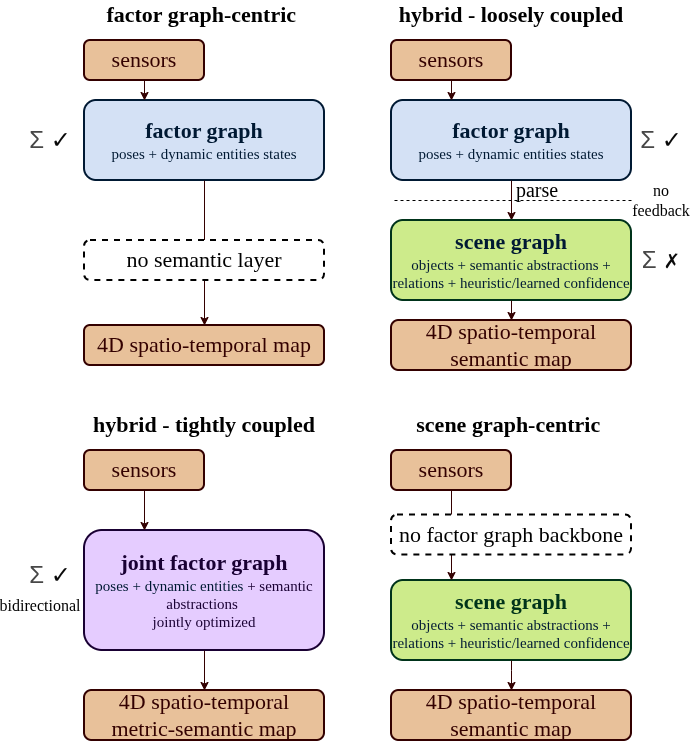
\includegraphics[width=0.9\columnwidth]{Figures/figure_architectural_patterns.png}
    \caption{Four distinct architectures have emerged throughout the literature for representing dynamic environment, specifically \textit{factor graph-centric} (top left), \textit{scene graph-centric} (bottom right), \textit{loosely coupled hybrid FG-SG} (top right) and \textit{tightly-coupled hybrid FG-SG} (bottom left).}
    \label{fig:architectural_patterns}
\end{figure}

\paragraph{Tightly-Coupled SLAMMOT (FG-centric)}
Systems in this pattern, like DynaSLAM II \cite{bescos_dynaslam_2021}, DynoSAM \cite{morris_dynosam_2025}, AirDOS \cite{qiu2022airdos}, BodySLAM \cite{henning_bodyslam_2022}, BodySLAM++ \cite{henning_bodyslam_2023}, Gou et al. \cite{gou_visual_2024}, adopt the joint-optimization approach detailed in Section \ref{sec:dynamics_representations_agents}, treating dynamic entities as first-class factor graph variables rather than outliers.% a probabilistic rigorous approach to dynamic agent handling.
%They jointly optimize camera pose, static landmarks, and dynamic entity trajectories within a unified factor graph, using spatio-temporal reprojection factors to introduce cross-terms that make self-localization and object tracking mutually reinforcing. 
%A defining characteristic of this pattern is that dynamic entities are treated as first-class factor graph variables rather than as outliers. 
The trade-off is that this template primarily addresses continuously moving agents, while semi-static displacement and long-term structural changes are typically outside its scope, and no explicit semantic abstraction layer is provided for higher-level reasoning tasks.

\paragraph{Layered Stack with FG Backbone ( loosely coupled hybrid FG-SG)}
Kimera \cite{rosinol_kimera_2021} and Hydra \cite{hughes_hydra_2022} exemplify a layered architecture in which a factor graph optimizer provides a globally consistent geometric foundation, while a separate scene graph parser constructs the semantic-relational superstructure. 
The advantage is modularity: the scene graph logic can be developed independently of the SLAM back-end. 
The disadvantage is one-directional information flow: the scene graph is informed by the factor graph, but semantic information rarely propagates back to improve localization, so geometric uncertainty never reaches the semantic layer.


\paragraph{Unified Optimizable Graph ( tightly-coupled hybrid FG-SG)}
S-Graphs \cite{bavle_s-graphs_2025} and DynEMo-SLAM \cite{giberna_dynemo-slam_2025} incorporate semantic entities directly as variables and factors within the same factor graph that optimizes robot poses. 
This enables bidirectional information flow: semantic structural priors constrain ego-trajectory estimation, while geometric observations refine semantic entity states. 
DynEMo-SLAM extends this template to dynamic entities by constraining entity pose variables with semantic motion priors and structural relations. 
The pattern is particularly expressive in environments where structural semantics are stable and informative, while its applicability to large-scale, dynamic outdoor settings, where the number and identity of semantic entities grow rapidly, has not yet been demonstrated.
%represent a tighter integration in which semantic entities are incorporated directly as variables and factors within the same factor graph that optimizes robot poses.
% This enables bidirectional information flow: semantic structural priors constrain ego-trajectory estimation, while geometric observation refine semantic entity states.
% Specifically, DynEMo-SLAM extends this template to dynamic entities by constraining entity pose variables with semantic motion priors and structural relations.
% The pattern is particularly expressive in environments where structural semantics are stable and informative. 
% However, its applicability to large-scale, dynamic outdoor settings, where the number and identity of semantic entities grow rapidly, has not yet been demonstrated. 

\paragraph{Belief-Augmented and Dynamic Scene Graph (SG-centric)}
DovSG \cite{yan_dynamic_2025}, Lost \& Found \cite{behrens_lost_2025}, BSG \cite{saucedo_estimating_2025}, Aion \cite{catalano_aion_2025}, and Functional Scene Graphs \cite{zhang_open-vocabulary_2025} emphasize the scene graph as a persistent and explicitly dynamic world model, maintained primarily through semantic reasoning and graph-level updates rather than joint probabilistic optimization.
Persistence, forgetting, and state transition are central to this pattern: Lost \& Found distinguishes object removal from occlusion through the containment mechanism described in Section \ref{sec:dyn_world_model_representations_scene_graphs}.
Aion further extends this paradigm by encoding temporal activity patterns directly into the scene graph structure. 
These approaches  support long-term object permanence, natural language grounding, and interaction aware updates. 
Their reliance on heuristic or learned confidence measures, rather than trajectory level covariances, reflects a different trade-off between semantic expressiveness and probabilistic state estimation.

% Several descriptive patterns emerge from the taxonomy. 
% \textbf{Factor-graph-based systems} predominantly focus on geometric consistency and probabilistic state estimation, often providing explicit uncertainty representations and strong guarantees for incremental inference. 
% These approaches naturally support continuous dynamics and tightly-coupled estimation of robot and object motion, but typically require additional abstraction layers to support high-level semantic reasoning.

% In contrast, \textbf{scene-graph-centric systems} emphasize structured, hierarchical representations of the environment, enabling symbolic queries, task-level reasoning, and interaction modeling. 
% These systems frequently support semi-static changes and long-term memory through explicit graph maintenance mechanisms, although uncertainty is often represented implicitly or heuristically rather than through fully probabilistic inference.

% \textbf{Hybrid architectures} combine these complementary strengths by grounding semantic entities in a probabilistic geometric backbone. 
% Such systems commonly employ factor graphs for metric consistency and temporal estimation, while leveraging scene graphs to organize entities across abstraction levels and support downstream decision-making. 
% The taxonomy shows that hybrid approaches tend to integrate incremental smoothing back ends with hierarchical graph structures and explicit maintenance policies, reflecting the increased complexity of jointly modeling geometry, semantics, and dynamics.

% Across all graph stacks, the comparison highlights consistent relationships between the type of dynamics addressed, the chosen association and inference strategies, and the intended downstream applications. 
% These recurring patterns provide a consolidated view of how graphical models are currently employed for dynamic world modeling in robotics.

% \subsection{Trends in Graph-based World Modeling}\label{sec:taxonomy_trends}


% \paragraph{From Closed-Vocabulary to Open-Vocabulary Association} 
% \textcolor{red}{\sout{Early dynamic SLAM systems defined a fixed ontology of entities types at design type, like pedestrians, vehicles, or furniture, and relied on classifiers trained on these predefined categories.
% More recent systems increasingly leverage vision-language embeddings, including CLIP-based representations and vision-language models, to support open-vocabulary perception and association. 
% Frameworks such as DovSG \cite{yan_dynamic_2025} and ConceptGraphs \cite{gu_conceptgraphs_2023} demonstrate that open-set object discovery and association can be integrated into real-time robotic systems, enabling world models to accommodate previously unseen categories without retraining.}}

% \paragraph{From Reactive Maps to Predictive Spatial Memory}
% \textcolor{red}{\sout{
% Early dynamic world models were predominantly reactive, updating internal representations only in response to incoming observations and answering queries about the current state of the environment.
% A clear trend in more recent work is the incorporation of predictive components that encode expectations about unobserved entities and future activity, of which Aion's flow statistics (discussed below) are a representative case\cite{catalano_aion_2025}.
% Belief Scene Graphs' blind nodes (Section \ref{sec:dyn_world_model_representations_scene_graphs}) similarly estimate likely object locations from learned co-occurrence patterns \cite{saucedo_estimating_2025}, while Gorlo et al. \cite{gorlo_long-term_2024} leverage relational scene context to forecast long-term human trajectories.
% Altogether, these approaches extend world models from reactive state estimates toward representations that encode spatio-temporal patterns. 
% }}

% \paragraph{From Static Hierarchy to 4D Spatio-Temporal Representations}
% \textcolor{red}{\sout{Conventional 3D scene graph formulations organize the environment into a spatial hierarchies, such as objects, places, rooms, and buildings, that are largely static in their structural definition.
% Recent work has shifted from this assumption by explicitly incorporating temporal information into the representation\cite{schmid_khronos_2024}.
% Aion\cite{catalano_aion_2025} is the clearest instance of this shift: by attaching time-dependent flow statistics directly to navigational nodes, it extends the scene graph into a four-dimensional representation that captures not only spatial structure but temporal patterns of activity.
% %, for instance, attaches time-dependent flow statistics directly to navigational nodes, effectively extending the scene graph into a four-dimensional representation that captures not only the spatial structure but also temporal patterns of activity.
% This shift reflects a broader trend toward world models that encode when and how frequently interactions occur, rather than treating temporal variation as a sequence of independent snapshots.}}


%%% OLD NOTES
% Hierarchical Abstraction: The shift from "flat" representations to hierarchical 3D Scene Graphs (3DSGs) allows robots to reason over spaces in terms humans understand (e.g., rooms, buildings) rather than just dense point clouds \cite{rosinol_3d_2020, rosinol_kimera_2021}.

% Uncertainty Modeling: While early systems like Kimera use explicit Bayesian updates for semantic mesh labeling \cite{rosinol_kimera_2021}, newer frameworks like Lost \& Found \cite{behrens_lost_2025} highlight that modeling uncertainty for tracked objects is a critical next step for handling ambiguous interactions.

% Efficiency in Inference: Morris et al. \cite{morris_importance_2024} demonstrate that using a Hybrid formulation (combining world-centric and object-centric views) significantly increases factor graph sparsity, allowing for incremental solvers like iSAM2 to achieve real-time performance that previously required heavy batch optimization.

% Open-Vocabulary Capabilities: Systems like DovSG \cite{yan_dynamic_2025} and ConceptGraphs \cite{gu_conceptgraphs_2023} leverage Vision-Language Models (VLMs) to handle object categories unforeseen at design time, making them far more adaptable to real-world household environments compared to older "closed-vocabulary" SLAM systems

% Geometric-Semantic Hybridization: The most robust systems, such as Kimera \cite{rosinol_kimera_2021} and DynoSAM\cite{morris_dynosam_2025}, leverage factor graphs as a low-level "geometric backbone" while employing 3D Scene Graphs (3DSGs) for high-level semantic reasoning. This allows for joint optimization of robot trajectories and dynamic agent motions, resolving the motion ambiguity inherent in dynamic SLAM.

% Persistence and Forgetting Policies: Lifelong autonomy frameworks like Lost \& Found \cite{behrens_lost_2025} implement specific logic to handle semi-static change. Decisions to maintain object permanence (via "contains" edges) or prune "stale" nodes are driven by geometric verification—distinguishing between "absence of evidence" (occlusion) and "evidence of absence" (removal) \cite{schmid_khronos_2024}.

% Probabilistic Expectation: Emerging works in Belief Scene Graphs utilize GCN-based link prediction to populate unobserved areas with "blind nodes"\cite{saucedo_estimating_2025}. This shifts the world model from a purely reactive map to a predictive memory structure capable of guiding active object search under partial observability.

% Transition to 4D Representations: Recent frameworks like Aion \cite{catalano_aion_2025} extend the hierarchical stack by attaching temporal flow dynamics (Maps of Dynamics) directly to navigational nodes. By learning directional flow statistics over daily or seasonal cycles, these 4D scene graphs enable proactive planning in highly populated, rhythmic environments.

% The "Moving" vs. "Movable" Distinction: Brink (2016)\cite{brink_using_2016} and Gomez et al. (2020)\cite{gomez_object-based_2020} move beyond simple outlier rejection by modeling an object's capability for movement (semi-static). This allows the robot to retain a chair in its map even when it is stationary, while remaining alert that its position might change.

% Complexity Management: Walcott-Bryant et al. (2012)\cite{walcott-bryant_dynamic_2012} highlight that for lifelong autonomy, a graph cannot grow indefinitely. They implement an explicit "forgetting" policy that prunes nodes where significant change has been detected, ensuring the optimization remains tractable.

% Decoupling Spatio-Temporal Inconsistencies: Khronos \cite{schmid_khronos_2024} introduces the concept of "object fragments" to factorize the spatio-temporal SLAM problem. By breaking observations into locally consistent fragments, the system can disentangle sensor noise from actual environmental changes.

% 4D Representations: Aion \cite{catalano_aion_2025} represents a significant shift by attaching temporal flow dynamics directly to the navigational nodes of a 3D scene graph. Instead of just tracking a single person, it learns the "rhythm" of the environment (e.g., a hallway that is busy every day at 9 AM), transforming a static 3DSG into a predictive 4D model.

% \begin{table*}[t]
%   \caption{TODOHow methods encode time, change, and maintenance in probabilistic (factor-graph) and structured (scene-graph) world models.}
%   \label{tab:taxonomy_dynamics}
%   \centering
%   \scriptsize
%   \setlength{\tabcolsep}{3pt}

%   \begin{tabularx}{\textwidth}{@{}l l l l l l l >{\raggedright\arraybackslash}X@{}}
%     \toprule
%     \textbf{Work} & \textbf{Temporal model} & \textbf{Change model} & \textbf{Existence} &
%     \textbf{Mode/state} & \textbf{Graph updates} & \textbf{Consistency} &
%     \textbf{Notes (what’s novel)} \\
%     \midrule

%     Behrens et al. (2025) &
%     \makecell[l]{Delayed online\\sliding window} &
%     \makecell[l]{Rigid 6DoF\\tracking} &
%     \makecell[l]{Heuristic\\interval} &
%     \makecell[l]{Open/closed\\(drawer)} &
%     \makecell[l]{Online relation\\updates} &
%     \makecell[l]{Transformable\\scene graph} &
%     \makecell[l]{Maintains object permanence for\\objects stored in drawers.} \\
%     \midrule

%     Bescos et al. (2020) &
%     \makecell[l]{Fixed temporal\\window (2s)} &
%     \makecell[l]{Constant-vel\\(motion)} &
%     \makecell[l]{Heuristic\\(keypoints)} &
%     \makecell[l]{3D bounding\\boxes} &
%     \makecell[l]{Dynamic keyframe\\insertion} &
%     \makecell[l]{Tightly-coupled\\joint BA} &
%     \makecell[l]{Mutual benefit between camera\\tracking and object tracking.} \\
%     \midrule

%     Brink (2016) &
%     \makecell[l]{Incremental BP\\(incremental)} &
%     \makecell[l]{Constant-vel\\+ accel} &
%     \makecell[l]{Binary latent\\variable ($x$)} &
%     \makecell[l]{Capable of\\move ($m$)} &
%     \makecell[l]{Incremental\\``forgetting''} &
%     \makecell[l]{Joint PGM\\segmentation} &
%     \makecell[l]{Explicitly models semi-static objects\\switching between states.} \\
%     \midrule

%     Morris et al. (2025) &
%     \makecell[l]{Incremental\\iSAM2} &
%     \makecell[l]{World-centric\\rigid motion} &
%     \makecell[l]{Heuristic\\tracklets} &
%     \makecell[l]{SE(3) pose\\+ motion} &
%     \makecell[l]{iSAM2 clique\\restructuring} &
%     \makecell[l]{Hybrid factor\\graph} &
%     \makecell[l]{Hybrid formulation improves sparsity\\for online incremental solving.} \\
%     \midrule

%     Rosinol et al. (2021) &
%     \makecell[l]{Fixed-lag (VIO)\\+ batch (DSG)} &
%     \makecell[l]{Continuous\\agent motion} &
%     \makecell[l]{Heuristic\\(semantic)} &
%     \makecell[l]{Panoptic\\labels} &
%     \makecell[l]{Mesh\\deformation} &
%     \makecell[l]{Hierarchical\\PGO} &
%     \makecell[l]{Integrates visual-inertial SLAM with\\dense human mesh (SMPL) tracking.} \\
%     \midrule

%     Gomez et al. (2020) &
%     \makecell[l]{Multi-session\\(offline sessions)} &
%     \makecell[l]{Relocated\\furniture} &
%     \makecell[l]{Probabilistic\\presence} &
%     \makecell[l]{Active vs.\\inactive} &
%     \makecell[l]{Online object\\merging} &
%     \makecell[l]{Object-based\\pose graph} &
%     \makecell[l]{Infers object ``movability'' based on\\long-term session experience.} \\
%     \midrule

%     Catalano et al. (2025) &
%     \makecell[l]{FreMEn frequency\\model} &
%     \makecell[l]{Navigational\\motion flows} &
%     \makecell[l]{Position-invariant\\hashing} &
%     \makecell[l]{Activity\\histograms} &
%     \makecell[l]{Temporal ownership\\transfer} &
%     \makecell[l]{Hydra-integrated\\PGO} &
%     \makecell[l]{First unification of Maps of Dynamics\\(MoD) and 3D Scene Graphs.} \\
%     \midrule

%     Walcott-Bryant et al. (2012) &
%     \makecell[l]{Incremental\\smoothing} &
%     \makecell[l]{Low-dynamic\\structural} &
%     \makecell[l]{Change node\\indicator ($c$)} &
%     \makecell[l]{Static, Added,\\Removed} &
%     \makecell[l]{Stale node\\pruning} &
%     \makecell[l]{Pose-graph\\optimization} &
%     \makecell[l]{Reduces graph size by removing stale\\nodes that no longer match reality.} \\
%     \bottomrule
%   \end{tabularx}

%   \vspace{2pt}

%   \begin{tabularx}{\textwidth}{@{}l >{\raggedright\arraybackslash}X@{}}
%     \textbf{Entries:} &
%     \textbf{Temporal model} (filtering vs smoothing, incremental vs batch);
%     \textbf{Change model} (continuous motion, displacement, structural change);
%     \textbf{Existence} (explicit latent variable or heuristic);
%     \textbf{Mode/state} (discrete states like open/closed);
%     \textbf{Graph updates} (node/edge addition/removal, compression);
%     \textbf{Consistency} (pose-graph optimization only vs joint graph optimization).
%     \\
%   \end{tabularx}
% \end{table*}


%% Conclusion and open challenges
\section{Open Challenges and Future Directions}\label{sec:challenges_future_works}
% The challenges outlined in this section directly relate to the three research questions posed in the Section \ref{sec:introduction}. 
% While Sections \ref{sec:dyn_world_model_representations}–\ref{sec:taxonomy} surveyed how dynamic world models are currently represented, constructed, and employed, the following discussion highlights where each of these questions remains only partially resolved. 
% In particular, the challenges below reflect open issues in (i) the integration of probabilistic and semantic representations (RQ1), (ii) robust construction and inference under severe dynamics and uncertainty (RQ2), and (iii) scalable, long-term use of dynamic world models in realistic robotic settings (RQ3).

% Despite significant progress in dynamic world modeling through probabilistic graphical representations, several fundamental challenges remain unresolved. 
% These challenges arise not from isolated algorithmic limitations, but from system‑level tensions between geometry and semantics, expressiveness and scalability, and short‑term estimation and long‑term autonomy. 
% This section outlines key open problems and promising research directions.
The works surveyed throughout this paper collectively demonstrate that probabilistic graph-based representations, i.e. combining factor graphs for geometric consistency with scene graphs for semantic abstraction, form a powerful paradigm for dynamic world modeling.
Yet the synthesis presented in Sections \ref{sec:dyn_world_model_representations}–\ref{sec:taxonomy} shows that this paradigm is still evolving. 
Several fundamental tensions remain unresolved: between geometric uncertainty and semantic expressiveness, between short-term agent tracking and lifelong change detections, between representational richness and computational tractability, and between single-robot operation and distributed autonomy.
This section organizes open challenges around the three research questions presented in Section \ref{sec:introduction}, clarifying where the field has progressed and where substantial work remains.
The challenges identified below are not independent.
The surveyed literature suggests a dependency structure rather than an absolute ranking of importance: reliable representation and estimation provide the basis for maintaining a consistent world model across time and agents, while such persistent representations are in turn required for reliable long-horizon exploitation.
Therefore, we distinguish (i) representation and estimation foundations, including uncertainty handling and robust association; (ii) maintenance and scalability challenges, including lifelong and distributed world modeling; and (iii) exploitation challenges, including uncertainty-aware planning, active perception, and task reasoning. 
Evaluation remains a cross-cutting requirement for assessing progress at all three levels.

\subsection{Representation: What to Model and How}\label{sec:open_challenges_representation}
\paragraph{Uncertainty Propagation}
The uncertainty types presented in Section \ref{sec:uncertainty_types} reveal that the FG-SG boundary is not a single uncertainty-propagation problem, but an interface among heterogeneous uncertainty types. 
Geometric-state uncertainty is comparatively well formalized within factor graphs, while semantic, association, existence, and relational uncertainties are represented using different probabilistic, learned, or heuristic mechanisms.
The central challenge is therefore not only to propagate covariance from the geometric layer, but to preserve and combine these heterogeneous beliefs as information crosses representation layers, as illustrated in Figure \ref{fig:FG_SG_uncertainty_boundary}.
Within the factor graph layer, uncertainty is principled: variables carry covariance (or information) matrices, factors are weighted according to measurement quality, and the Hessian of the non-linear least-squares problem propagates uncertainty globally through the graph \cite{dellaert_factor_2017}. 
In many hybrid systems, this stops at the interface between layers.
In layered-stack architectures, the most prevalent pattern, scene graph nodes are often instantiated from the geometric layer without inheriting pose uncertainty, such that a node extracted from a poorly constrained region of the map may be treated with the same confidence as one from a well-constrained area.
The unified optimizable graph pattern (e.g. S-Graphs \cite{bavle_s-graphs_2025}, DynEMo-SLAM \cite{giberna_dynemo-slam_2025}) partially mitigates this by representing semantic entities as factor graph variables. 
However, propagation of geometric uncertainty into \textit{relational} edges remains largely unaddressed (e.g. how certain is an \textit{on} relation given the covariance of both object pose nodes?).
The work of Millan-Romera et al. \cite{millanromera2026generationuncertaintyawarehighlevelspatial} is a step toward learned uncertainty estimates for semantic factors, but a general framework for uncertainty-aware scene-graph relations in dynamic environments does not yet exist.
Lost \& Found \cite{behrens_lost_2025} explicitly acknowledges that principled uncertainty quantification for tracked object states under interaction is a critical missing piece. 

A symmetric and largely unexamined problem exists at the opposite boundary too, between the perception front-ends and the factor graph itself.
The probabilistic machinery described in Section \ref{sec:background} rests on the assumption of zero-mean, temporally independent Gaussian measurement noise. 
As front-ends increasingly replace geometric primitives with learned geometric priors, this assumption is systematically violated: monocular depth foundation models, designed for single images, exhibit temporally inconsistent, flickering predictions across consecutive frames of a video \cite{video_depth_anything}, producing errors that are correlated over time and biased rather than zero-mean. 
Such errors are particularly damaging for dynamic entities, where the multi-view temporal fusion used to stabilize depth on static structure \cite{video_depth_anything} is unavailable, since independent object motion breaks the underlying temporal consistency constraints.
While learned depth and its uncertainty have been integrated into factor graph estimation for the static case \cite{bloesch2018codeslam} \cite{yang2020d3vo}, no equivalent framework calibrates the error statistics of learned geometric priors before their injection into dynamic-entity factors; the learned semantic covariances of \cite{millan-romera_learning_2024} address the semantic factor class only.

Closing these gaps, at both perception-factor graph and factor graph-scene graph boundaries, appears increasingly important for safety-critical deployment, where a robot must know not only \textit{what} its world model asserts, but also \textit{how much} to trust each assertion.

\paragraph{Non-Rigid Deformation Modeling}
The surveyed works are largely restricted to rigid-body dynamics: agents are modeled as rigid objects with 6-DoF pose trajectories, and structures are assumed piecewise rigid.
Non-rigid deformation, such as soft objects, cloth, liquids, deformable tools, remains almost entirely absent from probabilistic graph-based representations.
The body-model comparison in Section \ref{sec:dynamics_representations_agents} and Table \ref{tab:body_models} shows the spectrum: SMPL-family parametric models handle articulated human motion through skeletal kinematics, but treat the body surface as a predefined template with limited expressiveness for atypical morphologies or extreme deformation, while neural representations such as InstantAvatar \cite{jiang2022instantavatar} use subject-specific, higher dimensional representations that are less directly suited to integration as factor-graph state variables . 
Extending factor graphs to non-rigid entities requires defining suitable state spaces, motion priors, and measurement models, a challenge connected to the broader problem of deformable SLAM and still an open research frontier \cite{luca_carlone_slam_2025}.

\paragraph{Completeness of Dynamics Coverage}
As summarized by Table~\ref{tab:taxonomy_overview} (Section~\ref{sec:taxonomy}), no current system in the surveyed literature handles all three levels of dynamics (continuously moving agents, semi-static changes, and long-term structural evolution) simultaneously within a single unified probabilistic framework.
Systems that handle agents well (DynoSAM \cite{morris_dynosam_2025}, AirDOS \cite{qiu2022airdos}) typically do not model semi-static change; systems that handle semi-static change well (Khronos \cite{schmid_khronos_2024}, DynEMo-SLAM \cite{giberna_dynemo-slam_2025}) generally lack principled lifelong structural maintenance.
This gap reflects not only engineering constraints but also a deeper modeling difficulty: these dynamics occur at timescales that differ by order of magnitude, and the most effective probabilistic treatments are not trivially composable (e.g.  tightly-coupled factor-graph optimization for agent motion, persistence/decay mechanism for semi-static change, and inter session change detection with loop closure for structural evolution).
Unifying these regimes without sacrificing tractability remains an open problem.

\paragraph{Metric Scale Observability of Dynamic Entities under Minimal Sensing}
A structural pattern visible in Table \ref{tab:taxonomy_overview} but rarely made explicit in the literature is that the coverage of dynamics reported above is conditioned on metrically informative sensing: nearly all surveyed factor-graph formulations rely on stereo, RGB-D, or LiDAR input \cite{bescos_dynaslam_2021} \cite{morris_dynosam_2025} \cite{qiu2022airdos} \cite{gou_visual_2024}. 
This is not incidental. For an independently moving entity observed monocularly, the entity's structure scale, its motion, and the ego-motion scale are mutually entangled: unlike static structure, whose metric scale can be recovered from inertial measurements or transferred from the ego solution, the observed image displacements of a dynamic entity hinder ego-motion and object motion, making ratio-based scale transfer invalid.
The few monocular systems that do estimate dynamic entities resolve this only through strong metric priors: learned object dimensions \cite{yang_cubeslam_2019}, parametric human body models \cite{henning_bodyslam_2022} \cite{henning_bodyslam_2023}, or rigid-body kinematic structure \cite{qiu2022airdos}.
Existing analyses of dynamic SLAM formulations address coordinate frame choices \cite{morris_importance_2024} and estimation efficiency \cite{henein_dynamic_2020}, but to the best of our knowledge no principled observability analysis exists that characterizes which components of a dynamic entity's $SE(3)$ trajectory and scale are recoverable given a specific sensor suite, nor which shared static structure can serve as a metric anchor in the absence of direct depth. 
Closing this gap is a precondition for deploying the dynamic world models surveyed here on low-cost, weight-constrained platforms such as micro aerial vehicles and AR devices, where monocular-inertial sensing is often the only option.

% \paragraph{Gaussian Splatting as a Geometric Substrate}
% \textcolor{red}{\sout{
% 3D Gaussian Splatting (3DGS) \cite{kerbl_3d_2023}, a differentiable, high-fidelity alternative to point clouds and meshes, is an emerging geometric substrate not yet integrated with the probabilistic graph-based frameworks surveyed here.
% Dynamic extensions} \cite{matsuki_gaussian_2024} \cite{zheng_wildgs-slam_2025} \cite{li_dynagslam_2025}  \cite{xu_dg-slam_2024} } \textcolor{red}{\sout{separate static and dynamic Gaussian primitives, but largely follow an outlier-rejection paradigm rather than a probabilistic SLAMMOT formulation. 
% A natuaral next step is a tripartite representation in which a factor graph provides the probabilistic trajectory backbone, a Gaussian-splatting layer the geometric-photometric substrate, and a scene graph the relational semantic abstraction, raising open questions on propagating factor-graph uncertainty into Gaussian primitives, extracting scene-graph entities from Gaussian fields, and jointly optimizing all three layers in real time.}}
% A significant emerging direction, not yet fully integrated into the probabilistic graph-based frameworks, is 3D Gaussian Splatting (3DGS) \cite{kerbl_3dgs_2023} as a geometric scene representation for SLAM. 
% 3DGS represents the scene as a collection of differentiable 3D Gaussian primitives, each with position, covariance, opacity, and appearance parameters, enabling high-fidelity real-time rendering. 
% Its differentiability and explicit geometry make it attractive as an alternative to point clouds and meshes as the geometric substrate of hybrid world models. 
% Early GS-SLAM systems \cite{matsuki_gaussian_2024} report competitive tracking accuracy alongside substantially improved rendering quality. 
% Extensions to dynamic scenes, such as DG-SLAM \cite{xu_dg-slam_2024}, WildGS-SLAM \cite{zheng_wildgs-slam_2025}, DynaGSLAM \cite{li_dynagslam_2025}, suggest that Gaussian primitives can be separated into static and dynamic components and tracked over time, although many current systems still resemble the outlier-rejection paradigm (e.g. masking dynamic Gaussians) rather than integrating them into a probabilistic SLAMMOT formulation. 
% Semantic GS-SLAM approaches \cite{lu_gsff-slam_2025} \cite{li2024sgs} further embed feature fields into the Gaussian representation, moving toward the semantic abstraction needed for scene-graph construction. 
% A natural next step is a tripartite representation in which a factor graph provides the probabilistic trajectory backbone, a Gaussian-splatting layer provides the geometric-photometric substrate, and a scene-graph layer provides relational semantic abstraction. 
% Realizing this integration raises concrete open questions: how to propagate factor-graph uncertainty into Gaussian-primitive uncertainty, how to extract scene-graph entities from Gaussian fields in a way that respects probabilistic structure, and how to jointly optimize all three layers within real-time budgets.

\subsection{Construction and Maintenance: How to Build and Maintain}\label{sec:open_challenges_construction}
The maintenance challenges in this section build on the representation-level issues above. Uncertainty, association and entity-state errors that are unresolved within a single-session world model do not disappear when operation is extended over time or across robots. Instead, they can accumulate across graph updates, sessions and inter-robot exchanges.
Lifelong and distributed operation therefore introduce additional scalability and consistency requirements on top of these estimation foundations.

\paragraph{Scalable Lifelong Graph Maintenance}
Long-term autonomy requires world models that remain tractable and accurate across sessions separated by hours, days, or months.
DPG-SLAM \cite{walcott-bryant_dynamic_2012} established a core principle: a graph cannot grow indefinitely, and an explicit forgetting policy, such as pruning nodes when they no longer contribute topological information, is essential for lifelong operation.
LT-mapper \cite{kim2022lt} demonstrated this principle at large scale for outdoor LiDAR SLAM. 
However, as the dynamics and structural complexity of the environment increase, the decision between what to keep and what to discard becomes harder to resolve reliably.
Many existing forgetting policies are primarily geometric or heuristic, and do not explicitly reason about the downstream utility of information for future tasks.
A promising direction is task-informed graph maintenance \cite{maggio_clio_2024}, where the decision to retain, update or prune nodes is conditioned on anticipated task distributions, eventually linking memory management to the planning and interaction layers described in Sections \ref{sec:applications} and \ref{sec:querying_reasoning_action}.

\paragraph{Open-Vocabulary Association under Severe Dynamics}
The shift toward open-vocabulary perception is a significant advance, but current open-vocabulary systems are often evaluated under relatively controlled conditions.
Under severe dynamics, like dense crowd occlusion, rapid viewpoint change, and simultaneous motion of many agents, the vision-language embeddings used for association (e.g. CLIP features in \cite{yan_dynamic_2025}, \cite{gu_conceptgraphs_2023}) may become unstable, and the lack of closed-form data-association uncertainty increases vulnerability to catastrophic misassociations. 
Integrating open-vocabulary perception into principled multi-hypothesis association frameworks (Section \ref{sec:construction_pipeline_data_association}) within this domain remains open, as does the question of how to bound false-association rates in scenes with many visually similar entities in motion.

\paragraph{Multi-Robot Shared Dynamic World Models}
As shown in Table~\ref{tab:taxonomy_overview}, explicit multi-robot capability (MR) is rare. Among the surveyed systems CURB-SG \cite{greve_collaborative_2024} explicitly evaluates collaborative mapping. 
Multi S-Graphs \cite{fernandez-cortizas_multi_2024} demonstrates that semantic-relational information can be exchanged efficiently to improve map merging, but extending this to dynamic entity tracking, where an agent observed by robot \textit{A} must be correctly associated with the track maintained by robot \textit{B} despite occlusion, viewpoint and time differences, introduces cross-agent data-association challenges that remain largely unaddressed. 
PMBM-based formulations \cite{ge2025batch} offer a theoretically grounded starting point towards a distributed extension, but have not yet been coupled to scene-graph-level semantic reasoning and maintenance policies.

\subsection{Exploitation}
The applications surveyed in Section \ref{sec:applications}  show that hybrid representations can combine probabilistic geometric estimation with semantic-relational capabilities across a broad range of downstream tasks. 
Yet the exploitation layer reveals its own set of open challenges, which are distinct from the representation and maintenance gaps above: even a perfectly maintained world model cannot be fully exploited by current task-level systems.
These challenges therefore occupy a downstream level of the dependency structure: reliable representation and maintenance are necessary inputs to task-level reasoning, but are not sufficient to guarantee effective exploitation.

\paragraph{Uncertainty-Aware Downstream Tasks and Proactive Planning under Dynamics}
The probabilistic machinery underlying factor graphs produces rich uncertainty estimates, such as pose covariances and existence probabilities for dynamic entities, that are largely discarded at task execution time. 
In practice, planners exploit scene graph nodes as point estimates, manipulation systems act on deterministic object poses, and task reasoners treat scene state as binary truth, regardless of how well constrained the underlying map is. 
This disconnection is particularly problematic near the boundaries of map reliability, where sparse loop closures or recent dynamics induce high uncertainty but do not influence decision-making. 
Planning over scene graphs has begun to address graph updates \cite{ejaz2025situationallyawarepathplanningexploiting}, yet broader questions remain open: how map uncertainty should affect task selection, action sequencing, or the decision to actively seek additional observations. 
A closely related limitation appears in planning under dynamics. 
Current systems either replan reactively when scene graph nodes change or invalidate precomputed paths \cite{ejaz2025situationallyawarepathplanningexploiting}, while predictive approaches, such as Aion’s temporal flow statistics \cite{catalano_aion_2025} or trajectory forecasting from scene graph context \cite{gorlo_long-term_2024}, remain decoupled from probabilistic task planning. 
Bridging factor-graph uncertainty and predictive temporal models into task-level planning objectives, so that actions are conditioned on the expected future state of the world rather than its instantaneous estimate, remains a largely open challenge.

\paragraph{Closing the Exploitation-to-Representation Loop: Active Perception}
All surveyed systems are effectively open-loop between exploitation and representation: task execution consumes the world model but does not feed information back to guide its refinement. 
A robot that fails to grasp an object because its pose estimate was uncertain has acquired evidence about which part of the map is unreliable, but no current system uses task-execution outcomes to trigger targeted re-observation or prioritize re-mapping of specific regions. 
The active perception literature addresses related problems, but largely in isolation from the structured world models surveyed here. 
Coupling the task layer to the maintenance layer, so that downstream failures or high-uncertainty decisions trigger directed exploration to reduce map uncertainty in task-relevant regions, would close the loop between the three research questions. 
This direction is conceptually previewed by task-informed graph pruning in Clio \cite{maggio_clio_2024}, which uses task context to decide what to retain, but the inverse direction, using task failures to decide what to re-observe, remains entirely open.

\paragraph{Temporal Consistency of Language-Grounded Task Plans}
Systems like SayPlan \cite{rana2023sayplangroundinglargelanguage} and SG-Nav \cite{yin2024sgnav} ground natural language instructions in scene graph state to produce task plans. 
This grounding is computed at a single moment in time and assumed stable for the duration of task execution. 
In dynamic environments, however, the scene graph changes continuously: objects are displaced by human interaction, agents move, doors open and close. 
A task plan grounded in a scene graph that was valid at planning time may refer to entities or relations that no longer hold at execution time, leading to silent failures that are difficult to detect and recover from. 
No current system monitors the temporal consistency between an active task plan and the evolving world model, or triggers re-planning when the graph changes in ways that invalidate the current plan's preconditions. 
This is particularly acute for multi-step manipulation tasks in human-populated environments, where the interval between planning and execution may span multiple human interactions. 
The connection between dynamic graph update policies (Section~\ref{sec:construction_pipeline_graph_maintenance}) and plan validity monitoring is entirely unaddressed in the surveyed literature.

\paragraph{Evaluation Gap: Task Performance as a Function of World Model Quality}\label{sec:open_challenges_metrics_gap}
A methodological gap cuts across all exploitation challenges: there is currently no benchmark or evaluation protocol that measures downstream task performance as a function of world model accuracy under dynamics.
Task-conditioned evaluation is therefore cross-cutting rather than a final stage of this hierarchy: it is needed to determine whether progress at the representation, maintenance or exploitation level produces measurable improvements in robotic performance. 
A rigorous characterization of this propagation chain requires more than evaluating each module independently. 
Ideally, upstream perception quality should be perturbed or stratified systematically and its effect measured at successive levels: association accuracy, geometric state estimation, scene-graph correctness, and task success.
The surveyed literature rarely performs such end-to-end sensitivity analysis, making it difficult to determine which upstream errors dominate downstream robotic performance or where additional robustness provides the greatest practical benefit.
This limitation stems primarily from the lack of challenging datasets in which the tight integration of dynamic handling and reasoning is required for the system to succeed on them.
Most work relies on commonly used and accepted datasets (Section ~\ref{sec:evaluation_metrics_datasets}) which are not built to create a realistic, challenging scenario regarding the dynamicity level of the environment. 
This results in under-validated works or the requirement for them to generate self-collected datasets to showcase the effective benefit of the proposed contributions \cite{giberna_dynemo-slam_2025}.
This limitation is compounded by a more basic one: accurate 6-DoF ground truth for the dynamic entities themselves is essentially only available inside motion-capture volumes \cite{sturm_benchmark_2012}\cite{palazzolo2019iros}\cite{judd_oxford_2019}, restricting validation to room-scale scenes, or as human-annotated 3D bounding boxes in driving benchmarks\cite{geiger_are_2012}\cite{caesar_nuscenes_2019}, whose accuracy and domain do not transfer to indoor and mixed indoor-outdoor robotics. 
No existing dataset provides metrically accurate object trajectories for handheld or robot-mounted sequences at building scale, which is the regime targeted by most systems in Table \ref{tab:taxonomy_overview}, and a further reason why simulation\cite{rosinol_kimera_2021}\cite{tartanair2020iros} and self-collected data \cite{giberna_dynemo-slam_2025} dominate current evaluations.
Existing evaluation protocols (Section~\ref{sec:evaluation_metrics_protocols}) assess trajectory accuracy, map geometry, graph structure, and tracking metrics largely in isolation from task outcomes. 
The connection between, for instance, a 10\% increase in object pose RMSE under crowded dynamics and the resulting manipulation success rate degradation is not measured by any of the surveyed evaluation frameworks. 
This gap makes it difficult to quantify the practical benefit of more accurate dynamic world models for robotic autonomy, and to motivate the computational cost of the more expressive representations described in this survey. 
Developing task-conditioned evaluation protocols, where world model quality is assessed through its effect on downstream task success under varying levels of environmental dynamics, would provide a more grounded benchmark for future progress. 
This connects naturally to the consecutive task execution protocols already adopted by works like DovSG \cite{yan_dynamic_2025}, which could be extended to include controlled degradation of world model quality as an independent variable.

% \bigskip
% %% Conclusion
% The open challenges above allow the three research questions presented in Section \ref{sec:introduction} to be summarized. 
% Regarding \textit{which representations} are suited to dynamic environments, the taxonomy shows that no single graph stack dominates; instead, key limitations arise at the interfaces between paradigms (notably uncertainty transfer across the FG-SG boundary and incomplete coverage across dynamics timescales). 
% Regarding \textit{how representations can be constructed and maintained}, the pipeline is increasingly well understood for single sessions with moderate dynamics, but scalable lifelong maintenance, robust open-vocabulary association under severe dynamics, and multi-robot shared construction remain unresolved. 
% Regarding \textit{how representations can be exploited}, downstream capabilities are already broad, yet their reliability depends on representations that remain consistent under change and can quantify confidence across geometric and semantic layers. 
% In this context, tighter integration between probabilistic factor graphs, semantically rich scene graphs, and emerging dense geometric substrates, in our view, one of the central challenges, and a promising direction, for long-term robotic situational awareness in dynamic environments.


% Relating to RQ1 and RQ2, a central unresolved issue in hybrid world model is the \textbf{propagation of uncertainty across representational layers}. 
% Factor graphs provide well defined probabilistic semantics, enabling principled uncertainty estimation over robot poses, landmarks and dynamic entities.
% Scene graphs, on the other hand, typically operate at a symbolic or relational level, where uncertainty is either abstracted away or represented through heuristic confidence scores.

% Existing systems show this disconnection. 
% Kimera explicitly maintains Bayesian uncertainty at the geometric layer, but higher-level scene graph entities are largely deterministic abstractions of optimized geometry.
% On the other side, belief-augmented scene graph approaches highlight the importance of uncertainty for object persistence and prediction, yet lack a mechanism to ground this belief in trajectory-level covariances.
% Bridging this gap requires representations in which semantic entities inherit and transform uncertainty from underlying geometric estimates, enabling queries such as confidence-aware planning or risk-sensitive reasoning.

% Promising directions include dynamic or belief-augmented scene graphs with explicit probabilistic semantics, joint optimization of relational and geometric variables, and interfaces that translate continuous uncertainty into relational belief updates.
% However, a general, scalable solution for uncertainty-consistent FG-SG integration remains open.

\section{Conclusion}\label{sec:conclusion}
This review examined graph-based robotic world models for dynamic environments through three central questions: which representations are suitable, how they can be constructed and maintained, and how they can be exploited for downstream robotic tasks.
To support this analysis, we introduced a taxonomy organized around the temporal horizon of environmental dynamics and assessed factor graphs, scene graphs, and their hybrid combinations.
The surveyed literature shows that no single representation dominates across all forms and timescales of dynamics. 
Factor graphs provide a principled foundation for uncertainty-aware geometric estimation, whereas scene graphs enable semantic abstraction and relational reasoning.  Hybrid architectures can combine these complementary capabilities within a common world model, although the surveyed evidence does not establish their general superiority over alternative representations.

% \textcolor{red}{\sout{Construction and maintenance pipelines are increasingly mature for single-session operation under moderate dynamics. Nevertheless, scalable lifelong maintenance, robust open-vocabulary data association under severe dynamics, consistent uncertainty propagation across geometric and semantic layers, and distributed multi-robot construction remain unresolved.
% Although existing representations already support a broad range of downstream capabilities, including navigation, manipulation, prediction, and task planning, their reliability ultimately depends on maintaining consistency and quantifiable confidence as the environment evolves. 
% Overall, tighter integration among probabilistic factor graphs, semantically rich scene graphs, and emerging dense geometric representations constitutes a central research direction toward robust situational awareness}}
The open challenges analyzed in Section X reveal a dependency structure rather than a set of equally independent research directions.
At the representation and estimation level, reliable uncertainty handling, robust data association, and principled entity-state management are required to maintain a consistent dynamic world model.
Extending this consistency across longer temporal horizons and multiple robots introduces a second set of challenges related to lifelong maintenance, scalability, and distributed construction.
Downstream capabilities such as uncertainty-aware planning, active perception, and task reasoning build on these maintained representations, while introducing additional task-level challenges of their own.
Task-conditioned evaluation cuts across all three levels and is necessary to determine whether improvements in representation and maintenance translate into measurable gains in robotic performance.
Overall, the surveyed evidence indicates that progress toward robust long-term dynamic world models depends on strengthening these representation and maintenance foundations while developing evaluation protocols that expose their impact on downstream autonomy in dynamic environments.

% The open challenges above allow the three research questions presented in Section \ref{sec:introduction} to be summarized. 
% Regarding \textit{which representations} are suited to dynamic environments, the taxonomy shows that no single graph stack dominates; instead, key limitations arise at the interfaces between paradigms (notably uncertainty transfer across the FG-SG boundary and incomplete coverage across dynamics timescales). 
% Regarding \textit{how representations can be constructed and maintained}, the pipeline is increasingly well understood for single sessions with moderate dynamics, but scalable lifelong maintenance, robust open-vocabulary association under severe dynamics, and multi-robot shared construction remain unresolved. 
% Regarding \textit{how representations can be exploited}, downstream capabilities are already broad, yet their reliability depends on representations that remain consistent under change and can quantify confidence across geometric and semantic layers. 
% In this context, tighter integration between probabilistic factor graphs, semantically rich scene graphs, and emerging dense geometric substrates, in our view, one of the central challenges, and a promising direction, for long-term robotic situational awareness in dynamic environments.

% \section*{Acknowledgment}
% M.G. Author thanks Laura Ribeiro for her valuable help in proofreading this manuscript. 

\bibliographystyle{IEEEtran}
\bibliography{bibliography, references}


%\begin{thebibliography}{00}

%\bibitem{b1} G. O. Young, ``Synthetic structure of industrial plastics,'' in \emph{Plastics,} 2\textsuperscript{nd} ed., vol. 3, J. Peters, Ed. New York, NY, USA: McGraw-Hill, 1964, pp. 15--64.

%\end{thebibliography}

%\begin{IEEEbiography}[{\includegraphics[width=1in,height=1.25in,clip,keepaspectratio]{a1.png}}]{First A. Author} (M'76--SM'81--F'87) and all authors may include 
%biographies. Biographies are often not included in conference-related
%papers. This author became a Member (M) of IEEE in 1976, a Senior
%Member (SM) in 1981, and a Fellow (F) in 1987. The first paragraph may
%contain a place and/or date of birth (list place, then date). Next,
%the author's educational background is listed. The degrees should be
%listed with type of degree in what field, which institution, city,
%state, and country, and year the degree was earned. The author's major
%field of study should be lower-cased.

%The second paragraph uses the pronoun of the person (he or she) and not the 
%author's last name. It lists military and work experience, including summer 
%and fellowship jobs. Job titles are capitalized. The current job must have a 
%location; previous positions may be listed 
%without one. Information concerning previous publications may be included. 
%Try not to list more than three books or published articles. The format for 
%listing publishers of a book within the biography is: title of book 
%(publisher name, year) similar to a reference. Current and previous research 
%interests end the paragraph. The third paragraph begins with the author's 
%title and last name (e.g., Dr.\ Smith, Prof.\ Jones, Mr.\ Kajor, Ms.\ Hunter). 
%List any memberships in professional societies other than the IEEE. Finally, 
%list any awards and work for IEEE committees and publications. If a 
%photograph is provided, it should be of good quality, and 
%professional-looking. Following are two examples of an author's biography.
%\end{IEEEbiography}

\begin{IEEEbiography}[{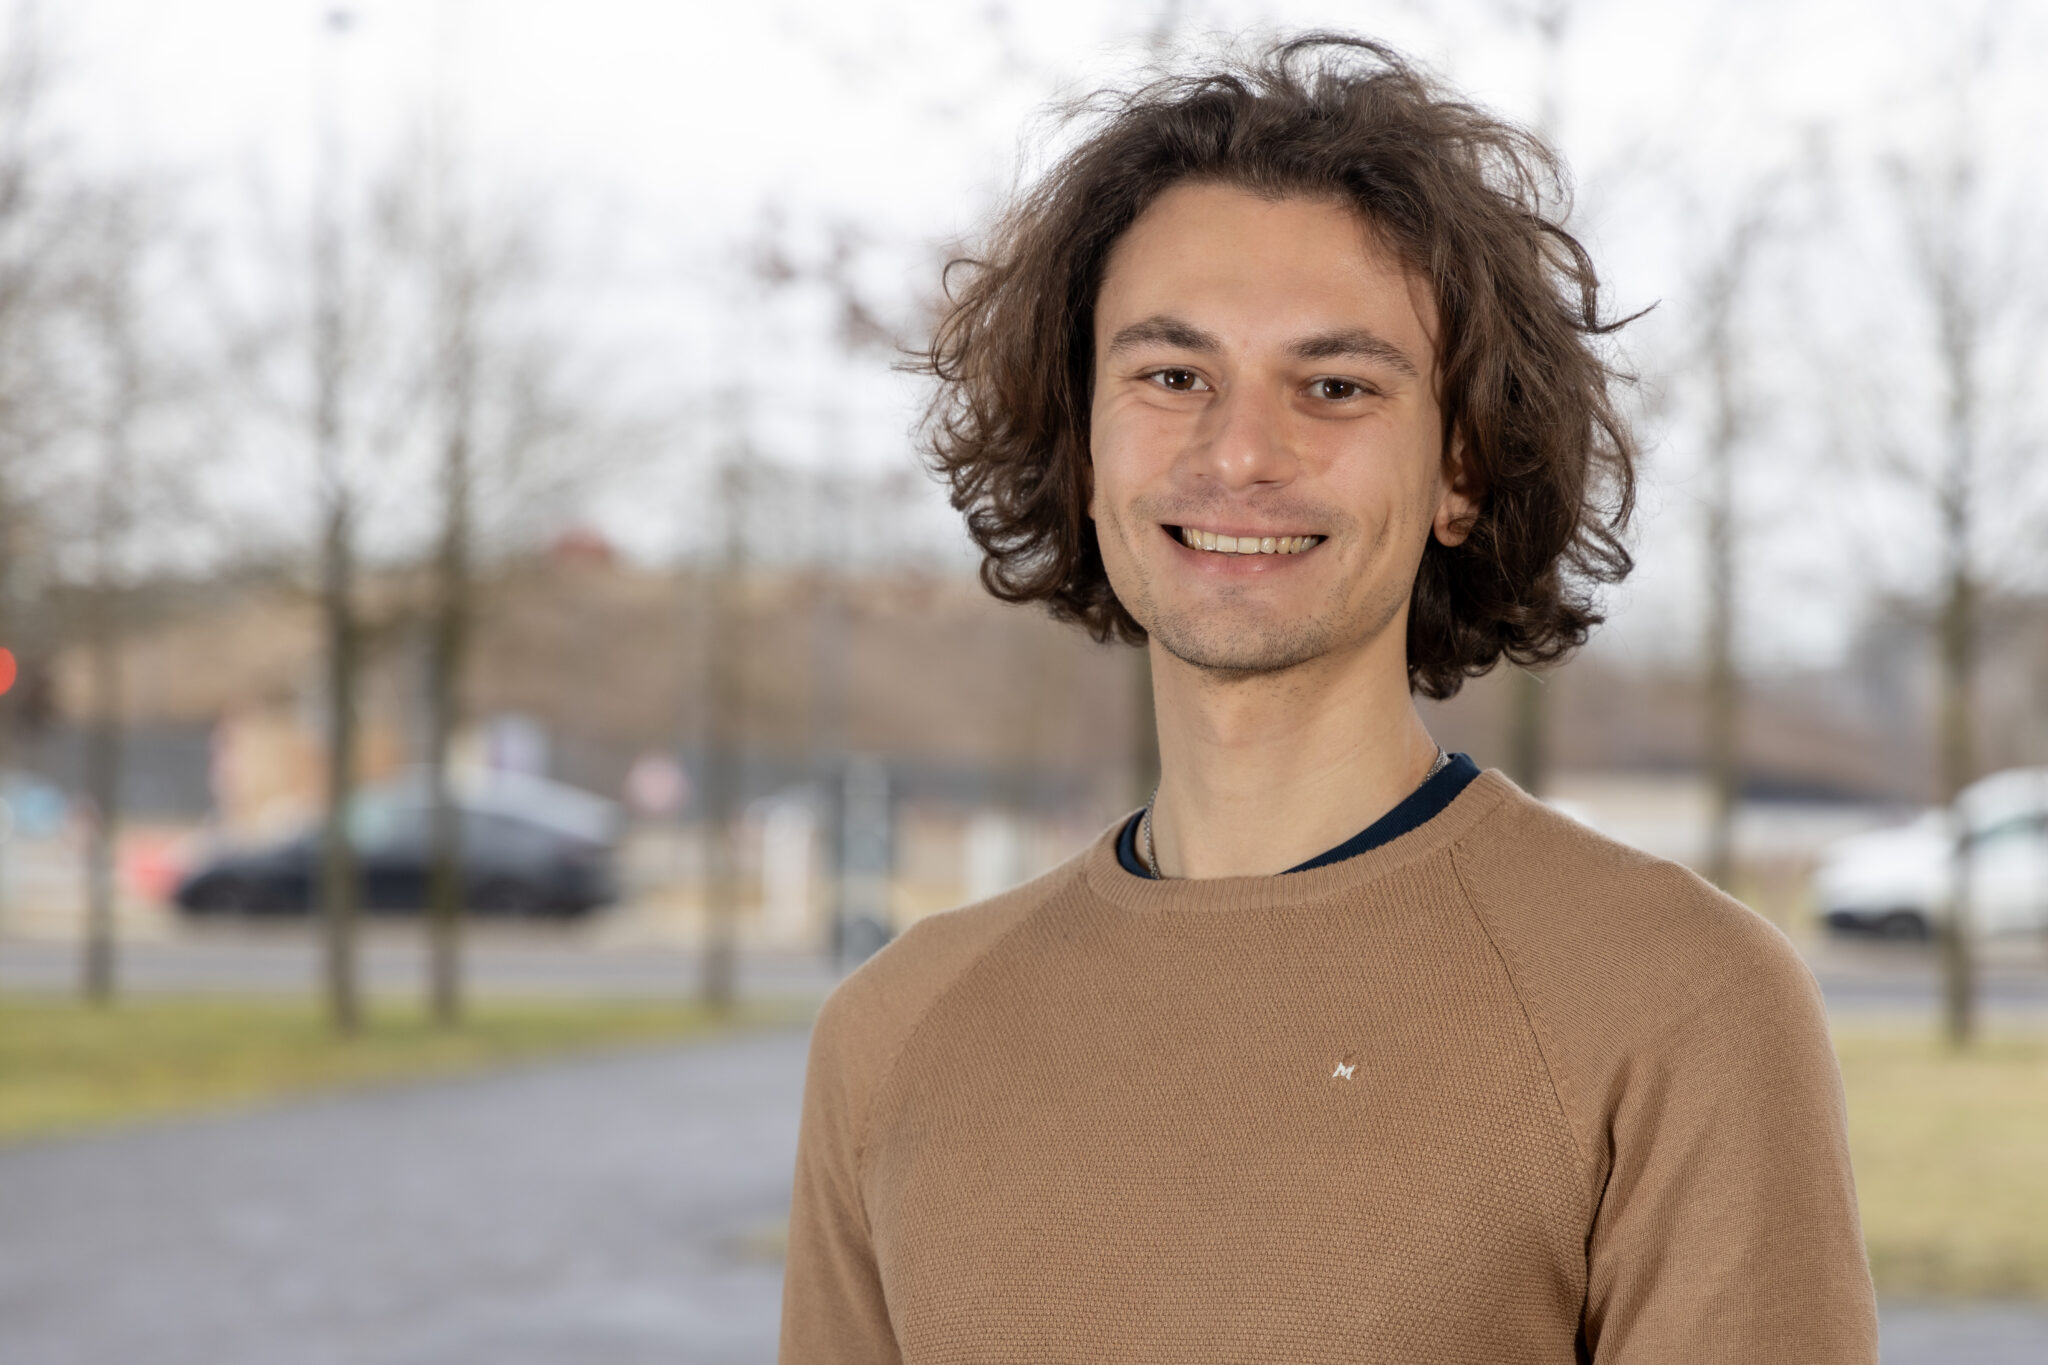
\includegraphics[width=1in,height=1.25in,trim={6.5cm 0 1.5cm 0},clip,keepaspectratio]{Pictures/marco_giberna_profile_picture_snt.jpeg}}]{Marco Giberna} received the B.S. degree in computer and electronic engineering from the University of Trieste, Italy, and the M.S. degree in computer and electronic engineering from the University of Trieste, Italy, in 2023. He is currently pursuing the Ph.D. degree with the Automation and Robotics Research Group (ARG), Interdisciplinary Centre for Security, Reliability and Trust (SnT), University of Luxembourg, headed by Prof. Holger Voos. His research interests include robotic perception, situational awareness for autonomous systems, and computer vision.
\end{IEEEbiography}

\begin{IEEEbiography}[{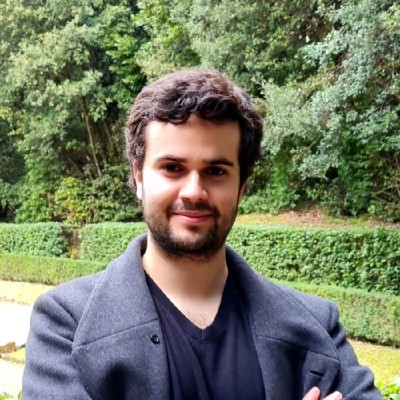
\includegraphics[width=1in,height=1.25in,trim={1cm 0 1cm 0},clip,keepaspectratio]{Pictures/MFC_PICTURE.jpeg}}]{Miguel Fernandez-Cortizas (Member, IEEE)} received the B.S. degree in industrial engineering, with a specialization in electronics and automation, and the M.S. and Ph.D. degrees in automation and robotics from the Universidad Politécnica de Madrid, Spain, in 2019, 2020, and 2025, respectively. During his doctoral studies, he was with the Computer Vision and Aerial Robotics Group (CVAR), working on multi-robot aerial systems and autonomous coordination. He has led the development of Aerostack2, a modular open-source framework for autonomous aerial robotics. Since 2025, he has been a Postdoctoral Researcher with the Automation and Robotics Research Group (ARG-SnT), University of Luxembourg, headed by Prof. Holger Voos, where he works on situational graphs and 3D scene graph SLAM for single and multi-robot systems. His research interests include increasing the situational awareness of autonomous robots through the development of cognitive architectures, semantic-relational SLAM, and collaborative SLAM algorithms.
\end{IEEEbiography}

\begin{IEEEbiography}[{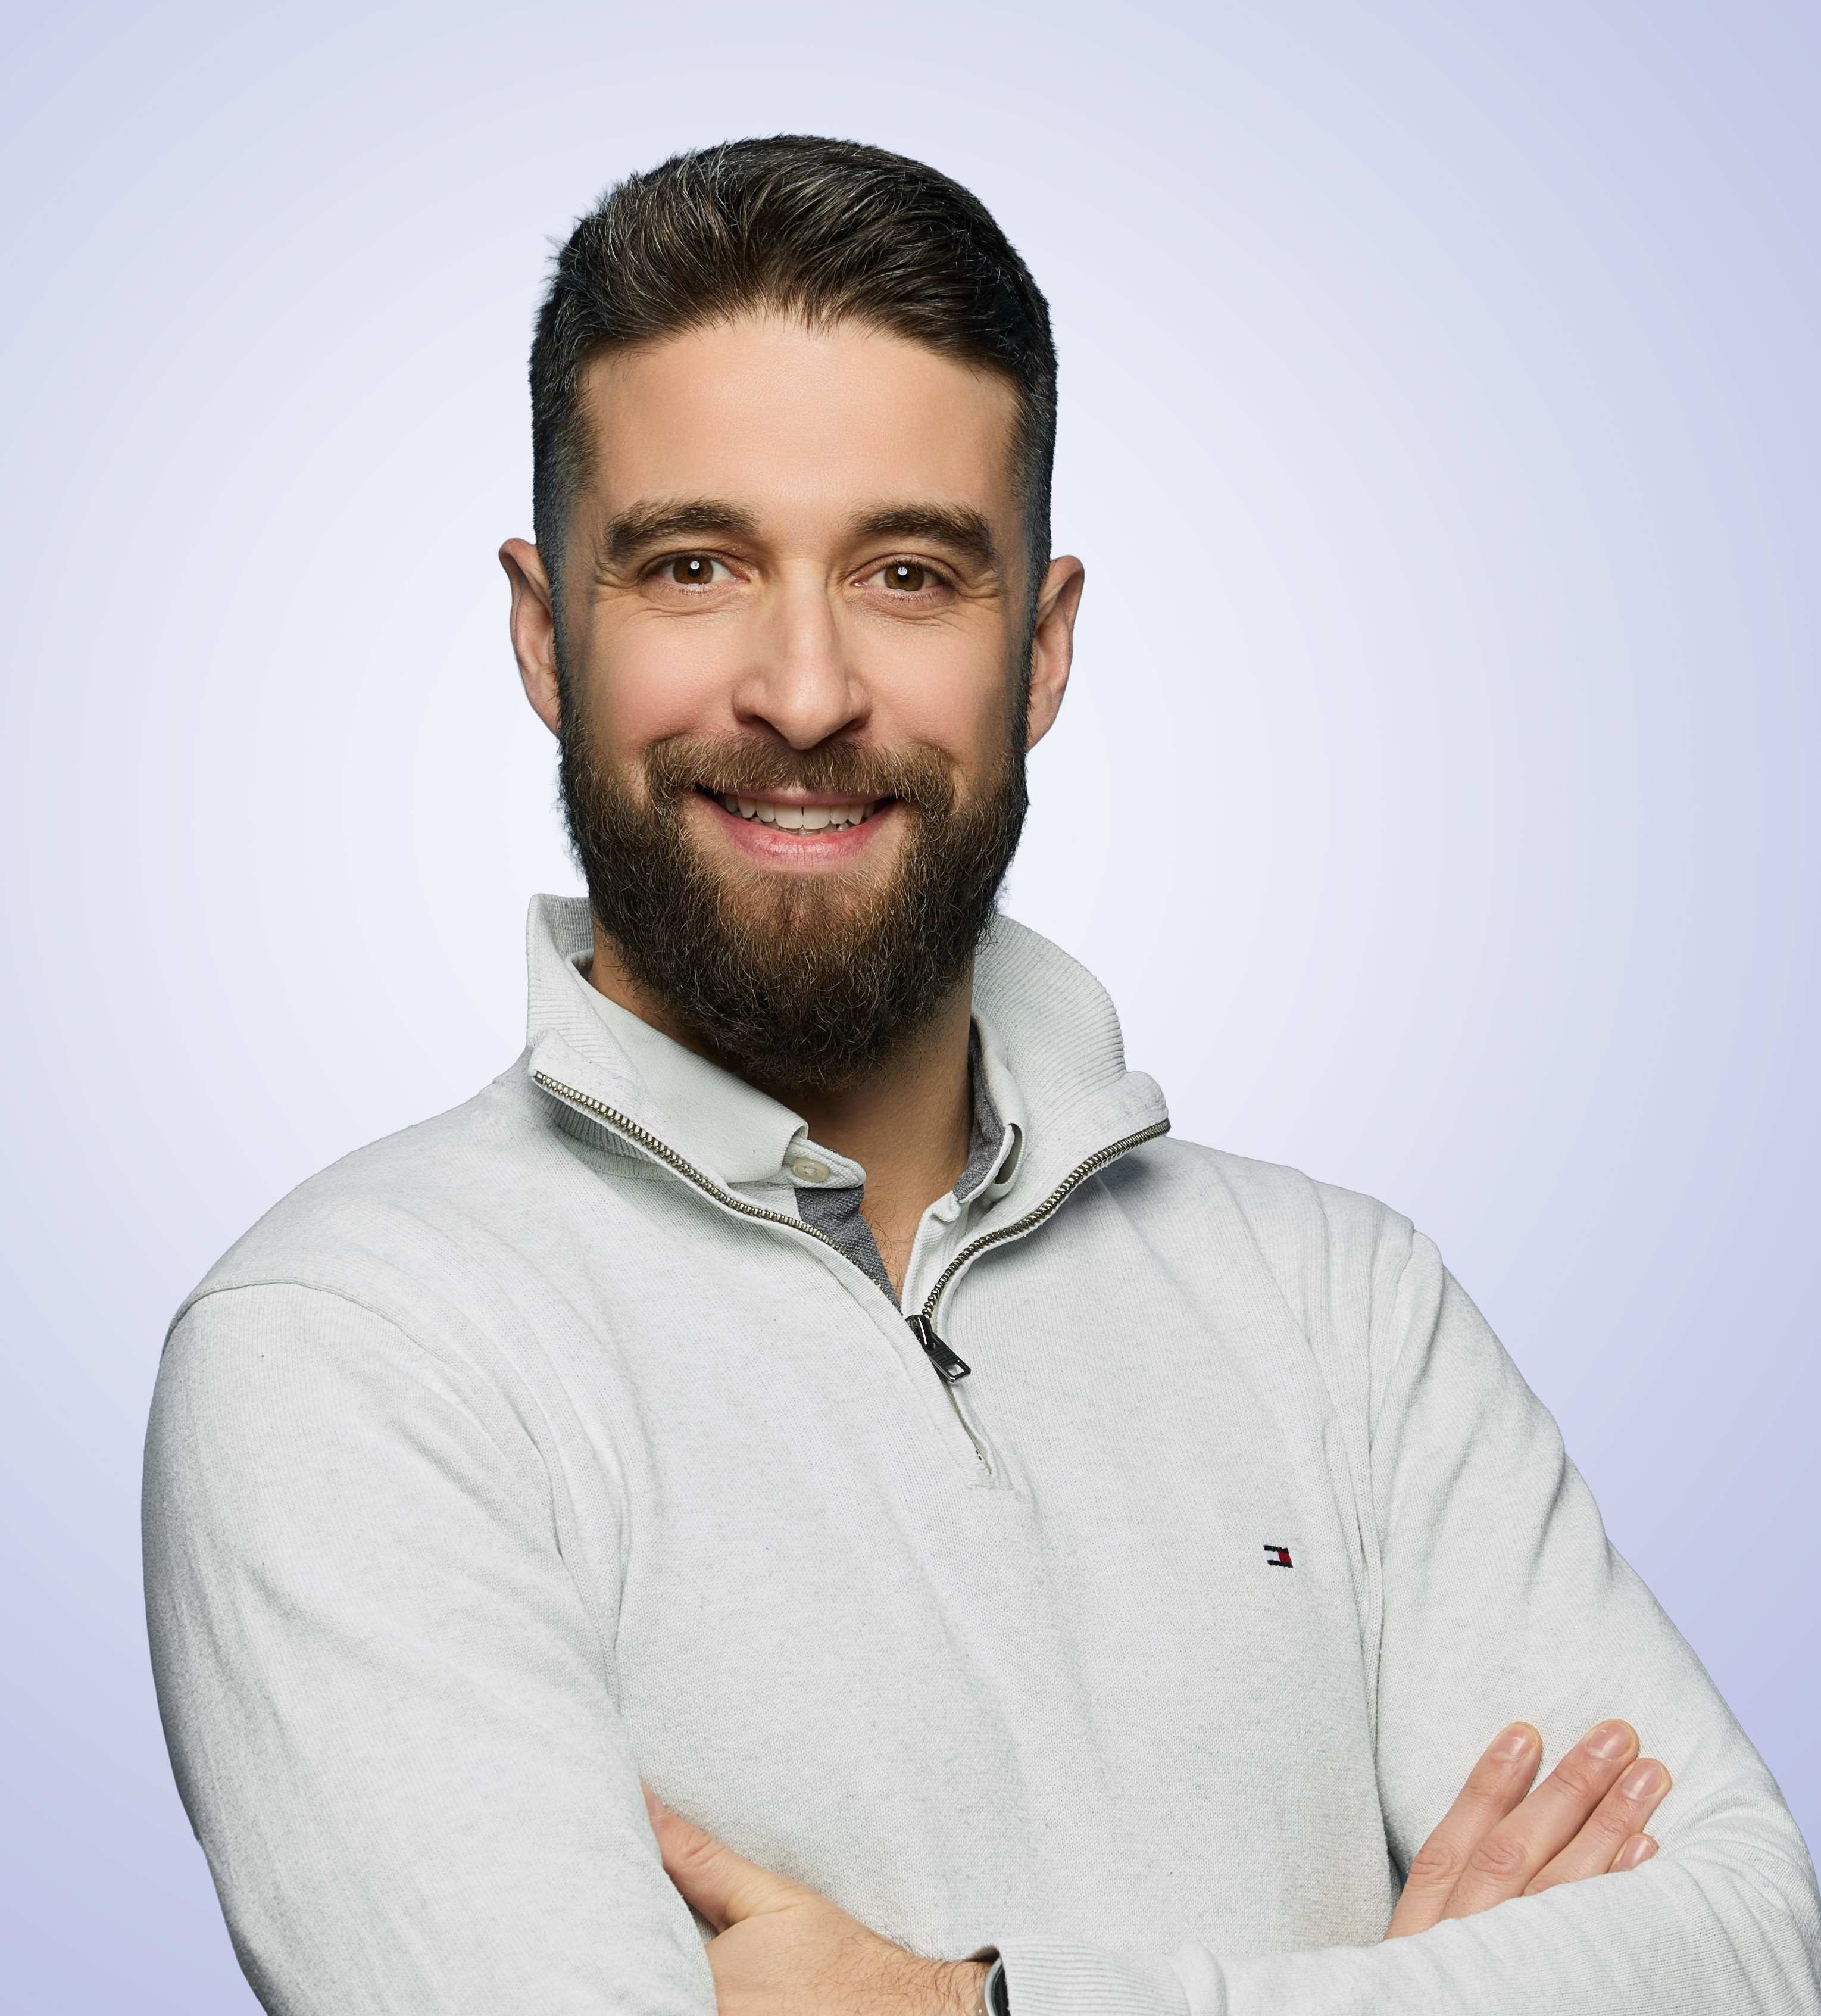
\includegraphics[width=1in,height=1.25in,trim={2.5cm 0 1cm 0},clip,keepaspectratio]{Pictures/SnT_Portraits_20255444_short.jpg}}]{Jose Luis Sanchez Lopez (Senior Member, IEEE)} is a Permanent Research Scientist at the SnT, University of Luxembourg, and deputy head of its Automation \& Robotics Research Group. He received his PhD in Robotics from the Technical University of Madrid in 2017 and has since been with the University of Luxembourg, with visiting research stays at H BRS, INRIA Rennes, and the University of Zaragoza. His research focuses on enhancing the autonomy, situational understanding, and decision-making capabilities of mobile robots and multi-robot systems for real-world applications. He has authored over 120 peer-reviewed publications, holds one patent, and contributes several open source software components. He has participated in multiple national and European research projects, securing more than €1.8M in competitive funding, and currently supervises 15 PhD students (5 as main supervisor). He serves the research community as an expert evaluator for funding agencies such as the European Commission; with editorial roles for top-tier journals, such as IEEE RA-L and Springer JINR, and conferences, such as IROS; workshop organizer in conferences such as ICRA; and as a PhD thesis committee member. He also teaches at the bachelor and master levels at the University of Luxembourg and engages in outreach activities, including serving as one of Luxembourg’s National Coordinators for the European Robotics Week.
\end{IEEEbiography}

\begin{IEEEbiography}[{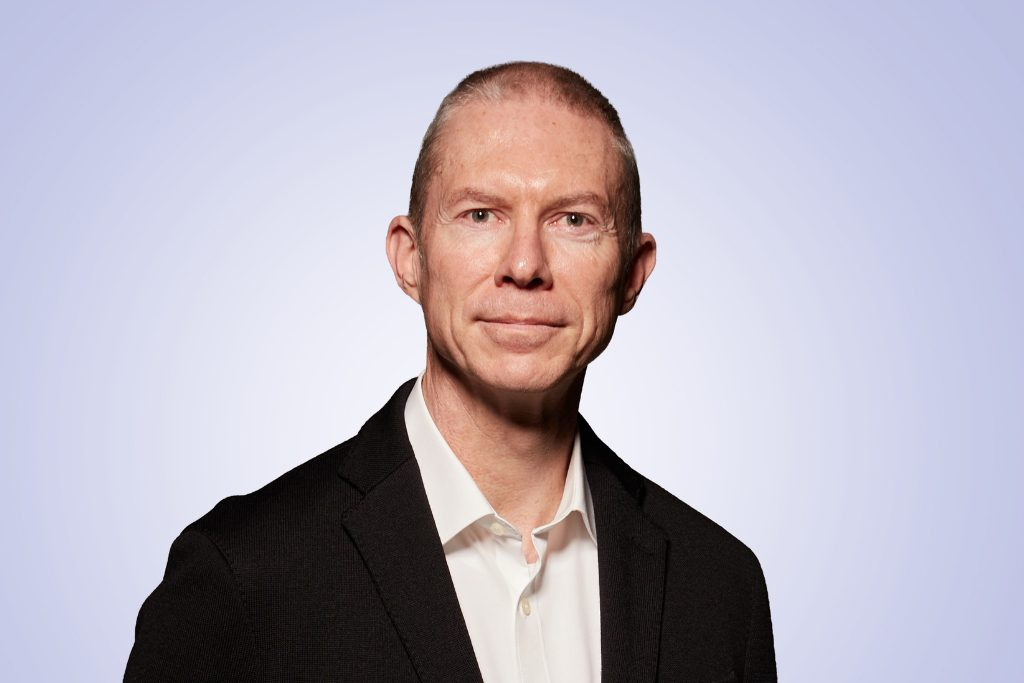
\includegraphics[width=1in,height=1.25in,trim={5cm 0 7cm 0},clip,keepaspectratio]{Pictures/holger_voos_snt.jpeg}}]{Holger Voos (Member, IEEE)} received the Dipl.-Ing. degree in electrical engineering from Saarland University and the Dr.-Ing. degree in automatic control from the Technical University of Kaiserslautern, Germany. From 2000 to 2004, he was with Bodenseewerk Gerätetechnik GmbH, Germany, as a Systems Engineer, and the Project Manager in aerospace and robotics research and development. From 2004 to 2010, he was a Professor and the Head of the Mobile Robotics Laboratory, University of Applied Sciences Ravensburg-Weingarten, Germany. Since 2010, he has been a Full Professor with the University of Luxembourg and the Head of the Automation and Robotics Research Group, Interdisciplinary Centre for Security, Reliability and Trust (SnT). From 2020 to 2024, he was the Founding Course Director of the New Interdisciplinary Space Master (ISM) Program, Faculty of Science, Technology and Medicine (FSTM). He is the author or co-author of more than 300 publications, comprising books, book chapters, journal and conference papers. His research interests include situational awareness and motion planning and control for autonomous vehicles and robots, and distributed and networked control and automation.
\end{IEEEbiography}

\EOD

\end{document}
